%% ----------------------------------------------------------------
%% Thesis.tex -- MAIN FILE (the one that you compile with LaTeX)
%% ---------------------------------------------------------------- 

% Set up the document
\documentclass[a4paper, 11pt, oneside]{Thesis}  % Use the "Thesis" style, based on the ECS Thesis style by Steve Gunn
\graphicspath{Figures/}  % Location of the graphics files (set up for graphics to be in PDF format)

% Include any extra LaTeX packages required
%\usepackage[square, numbers, comma, sort&compress]{natbib}  % Use the "Natbib" style for the references in the Bibliography
\usepackage{natbib}  % Use the "Natbib" style for the references in the Bibliography
\usepackage{verbatim}  % Needed for the "comment" environment to make LaTeX comments
\usepackage{vector}  % Allows "\bvec{}" and "\buvec{}" for "blackboard" style bold vectors in maths
\hypersetup{urlcolor=blue, colorlinks=true}  % Colours hyperlinks in blue, but this can be distracting if there are many links.


\usepackage[spanish]{babel}
\usepackage[utf8x]{inputenc}
\usepackage{enumerate}
\usepackage{float}
\usepackage{graphicx,subfigure}
%% ----------------------------------------------------------------
\begin{document}
	
	
\frontmatter      % Begin Roman style (i, ii, iii, iv...) page numbering



% Set up the Title Page
\title  {Detección \textit{in Silico} de Neoantígenos Utilizando Transformers y Transfer Learning en el Marco de Desarrollo de Vacunas Personalizadas para Tratar el Cáncer}
\authors  {\texorpdfstring
            {\href{vmachacaa@unsa.edu.pe}{Vicente Machaca Arceda}}
            {Author Name}
            }
\addresses  {\groupname\\\deptname\\\univname}  % Do not change this here, instead these must be set in the "Thesis.cls" file, please look through it instead
\date       {\today}
\subject    {}
\keywords   {}

\maketitle
%% ----------------------------------------------------------------

\setstretch{1.3}  % It is better to have smaller font and larger line spacing than the other way round

% Define the page headers using the FancyHdr package and set up for one-sided printing
\fancyhead{}  % Clears all page headers and footers
\rhead{\thepage}  % Sets the right side header to show the page number
\lhead{}  % Clears the left side page header





\pagestyle{fancy}  % Finally, use the "fancy" page style to implement the FancyHdr headers

%% ----------------------------------------------------------------
% Declaration Page required for the Thesis, your institution may give you a different text to place here
\Declaration{

\addtocontents{toc}{\vspace{1em}}  % Add a gap in the Contents, for aesthetics

Yo, Vicente Machaca Arceda, declaro que la tésis titulada, `Detección \textit{in Silico} de Neoantígenos Utilizando Transformers y Transfer Learning en el Marco de Desarrollo de Vacunas Personalizadas para Tratar el Cáncer' y el trabajo presentado en este, son de mi propiedad intelectual y confirmo que:

\begin{itemize} 
\item[\tiny{$\blacksquare$}] Este trabajo fue desarrollado durante mi candidatura a grado de doctor de esta universidad.
 
\item[\tiny{$\blacksquare$}] Ninguna parte de esta tésis ha sido presentado para otro grado de esta universidad o cualquier otra institución.
 
\item[\tiny{$\blacksquare$}] Cuando cito a otros autores, las fuentes has sido brindadas y con excepción de estas citas, mi trabajo es de mi autoría.
 
\item[\tiny{$\blacksquare$}] He agradecido las principales fuentes de ayuda.
 
\item[\tiny{$\blacksquare$}] En caso de que mi tesis haya sido desarrollado con un equipo de trabajo, yo he sido claro y he detallada la parte exacta de mi autoría.
\\
\end{itemize}
 
 
Firma:\\
\rule[1em]{25em}{0.5pt}  % This prints a line for the signature
 
Fecha:\\
\rule[1em]{25em}{0.5pt}  % This prints a line to write the date
}
\clearpage  % Declaration ended, now start a new page

%% ----------------------------------------------------------------
% The "Funny Quote Page"
\pagestyle{empty}  % No headers or footers for the following pages

\null\vfill
% Now comes the "Funny Quote", written in italics
\textit{``Con fe, disciplina y desinteresada devoción al deber, no hay nada que merezca la pena que no puedas lograr.''}

\begin{flushright}
Muhammad Ali Jinnah
\end{flushright}

\vfill\vfill\vfill\vfill\vfill\vfill\null
\clearpage  % Funny Quote page ended, start a new page
%% ----------------------------------------------------------------


\pagestyle{empty}  % Page style needs to be empty for this page
\dedicatory{Dedico este trabajo a mi esposa Pamela Laguna Laura, quien me ha acompañado durante todo este proceso, me ha motivado y sobre todo me ha dado su amor,  me ha ayudado a prevalecer y siempre seguir adelante. De igual forma, a mis padres Vicente Machaca Chino y Victoria Arceda Arenas, de ellos he aprendido el valor de la disciplina, la fuerza por emprender y la importancia de los valores sin importar las circunstancias; gracias a ellos he logrado cumplir mis objetivos. }

\clearpage 

% The Abstract Page
\addtotoc{Resumen}  % Add the "Abstract" page entry to the Contents
\abstract{
\addtocontents{toc}{\vspace{1em}}  % Add a gap in the Contents, for aesthetics

El cáncer es el mayor problema de salud mundial en la actualidad, frente a esto han surgido nuevos tratamientos basados en inmunoterapia como el desarrollo de vacunas personalizadas basadas en neoantígenos. Sin embargo, el proceso para identificar neoantígenos, es complejo y existen varias etapas para lograrlo, desde el secuenciamiento de muestras tumorales, alineamiento con muestras de tejido saludable, identificación y anotación de mutaciones, para luego proseguir con la predicción de la unión de péptidos con el MHC y posteriormente la unión del pMHC con el TCR. Si esta unión procede, el péptido en cuestión es un fuerte candidato a neoantígeno. En este proceso, una de las fases más críticas es la predicción de la unión pMHC, lo cuál ha motivado el desarrollo de esta tesis. 

Además, las redes neuronales Transformers han revolucionado el campo del procesamiento natural del lenguaje y se han aplicado en muchas otras áreas como en Proteómica. Esto porque las proteínas al ser representadas como secuencias de aminoácidos, son muy similares a las secuencias de palabras en una oración. Es así, que otras investigaciones han aplicado el uso de Transformers y redes neuronales con mecanismos de atención para la predicción de la unión pMHC. Adicionalmente, existen modelos pre-entrenados como TAPE, ProtBert y ESM2, estos han sido entrenados con grandes volúmenes de datos para varias tareas de Proteómica. Basados en lo anterior, en esta tesis se propone el uso de aplicar \textit{fine-tuning} a TAPE, ProtBert, ESM2(t6), ESM2(t12), ESM2(t30) y ESM2(t33) para la tarea de predicción de la unión pMHC, el \textit{fine-tunning} consistió en agregar un bloque BiLSTM al final del modelo. Además, se ha evaluado el uso de \textit{Gradient Accumulation Steps} (GAS) y una metodología de congelamiento de capas.

Luego de los experimentos, los modelos con mejores resultados fueron TAPE-GAS, que resultó de aplicar GAS a TAPE y ESM2(t6)-Freeze, que resultó de aplicar la metodología de congelamiento a ESM2. Finalmente, se compararon estos modelos con los métodos de mejor resultado en el estado del arte, tales como: NetMHCpan4.1, MHCflurry2.0, ACME, Anthem y MixMHCpred2.2. Al finalizar los experimentos, TAPE-GAS y ESM2-Freeze superaron a los otros métodos en \textit{accuracy}, AUC, \textit{presicion, f1-score} y MCC. 






}

\clearpage  % Abstract ended, start a new page
%% ----------------------------------------------------------------

\setstretch{1.3}  % Reset the line-spacing to 1.3 for body text (if it has changed)

% The Acknowledgements page, for thanking everyone
%\acknowledgements{
%\addtocontents{toc}{\vspace{1em}}  % Add a gap in the Contents, for aesthetics

%Dedico este trabajo a mis padres Vicente Machaca Chino y Victoria Arceda Arenas, de ellos he aprendido el valor de la disciplina, la fuerza por emprender y la importancia de los valores; gracias a ellos he logrado cumplir mis objetivos. De igual forma, dedico este trabajo a mi esposa Pamela Laguna Laura, quien me ha acompañado durante todo este proceso, me ha motivado a seguir y sobre todo me ha dado su amor, que me ha ayudado a prevalecer y siempre seguir adelante.  \\ 

%}
%\clearpage  % End of the Acknowledgements
%% ----------------------------------------------------------------

\pagestyle{fancy}  %The page style headers have been "empty" all this time, now use the "fancy" headers as defined before to bring them back


%% ----------------------------------------------------------------
\lhead{\emph{Contents}}  % Set the left side page header to "Contents"
\tableofcontents  % Write out the Table of Contents

%% ----------------------------------------------------------------
\lhead{\emph{List of Figures}}  % Set the left side page header to "List if Figures"
\listoffigures  % Write out the List of Figures

%% ----------------------------------------------------------------
\lhead{\emph{List of Tables}}  % Set the left side page header to "List of Tables"
\renewcommand{\listtablename}{Índice de tablas}
\renewcommand{\tablename}{Tabla}
\listoftables  % Write out the List of Tables

%% ----------------------------------------------------------------
\setstretch{1.5}  % Set the line spacing to 1.5, this makes the following tables easier to read
\clearpage  % Start a new page
\lhead{\emph{Abreviaciones}}  % Set the left side page header to "Abbreviations"
\listofsymbols{ll}  % Include a list of Abbreviations (a table of two columns)
{
% \textbf{Acronym} & \textbf{W}hat (it) \textbf{S}tands \textbf{F}or \\
%\textbf{LAH} & \textbf{L}ist \textbf{A}bbreviations \textbf{H}ere \\

\textbf{ANN}		& Artificial Neural Network \\
\textbf{AUC}		& Area Under the Curve\\
\textbf{BERT}   & Bidirectional Encoder Representations from Transformers \\

\textbf{bp}		& Base pair in DNA \\
\textbf{CNN}		& Convolutional Neural Network \\
\textbf{DNN}		& Deep Neural Network \\
\textbf{DNA}		& Deoxyribonucleic Acid \\

\textbf{GNN}		&  Graph Neural Netowrk\\
\textbf{G-BERT}		&  Graph Bidirectional Encoder Representations from Transformers\\
\textbf{HLA}		& Human Leukocyte Antigens 		\\
\textbf{MCC} 		& Matthews Correlation Coefficient \\
\textbf{MHC-I}		& Major Histocompatibility Complex Class I		\\
\textbf{MHC-II}		& Major Histocompatibility Complex Class II		\\
\textbf{MHC-III}		& Major Histocompatibility Complex Class III		\\
\textbf{mRNA}		& Messenger Ribonucleic Acid \\
\textbf{NLP}		& Natural Language Processing	\\
\textbf{pMHC}		& Peptide-MHC ligand\\
\textbf{pMHC-TCR}    & pMHC T-cell receptor ligand\\
\textbf{RNA}		& Ribonucleic Acid \\
\textbf{RoBERTa}     & Optimized BERT \\
\textbf{RSL}     & Revisión Sistemática de la Literatura \\
\textbf{tRNA}		& Transfer Ribonucleic Acid \\
\textbf{TCR}			& T-cell receptor \\

}
\clearpage

%% ----------------------------------------------------------------
%\clearpage  % Start a new page
%\lhead{\emph{Physical Constants}}  % Set the left side page header to "Physical Constants"
%\listofconstants{lrcl}  % Include a list of Physical Constants (a four column table)
%{
% Constant Name & Symbol & = & Constant Value (with units) \\
%Speed of Light & $c$ & $=$ & $2.997\ 924\ 58\times10^{8}\ \mbox{ms}^{-\mbox{s}}$ (exact)\\

%}

%% ----------------------------------------------------------------
%\clearpage  %Start a new page
%\lhead{\emph{Symbols}}  % Set the left side page header to "Symbols"
%\listofnomenclature{lll}  % Include a list of Symbols (a three column table)
%{
% symbol & name & unit \\
%$a$ & distance & m \\
%$P$ & power & W (Js$^{-1}$) \\
%& & \\ % Gap to separate the Roman symbols from the Greek
%$\omega$ & angular frequency & rads$^{-1}$ \\
%}
%% ----------------------------------------------------------------
% End of the pre-able, contents and lists of things
% Begin the Dedication page

\setstretch{1.3}  % Return the line spacing back to 1.3

%\pagestyle{empty}  % Page style needs to be empty for this page
%\dedicatory{Dedico este trabajo a mis padres Vicente Machaca Chino y Victoria Arceda Arenas, de ellos he aprendido el valor de la disciplina, la fuerza por emprender y la importancia de los valores; gracias a ellos he logrado cumplir mis objetivos. De igual forma, dedico este trabajo a mi esposa Pamela Laguna Laura, quien me ha acompañado durante todo este proceso, me ha motivado a seguir y sobre todo me ha dado su amor, que me ha ayudado a prevalecer y siempre seguir adelante. \ldots}

\addtocontents{toc}{\vspace{2em}}  % Add a gap in the Contents, for aesthetics


%% ----------------------------------------------------------------
\mainmatter	  % Begin normal, numeric (1,2,3...) page numbering
\pagestyle{fancy}  % Return the page headers back to the "fancy" style

% Include the chapters of the thesis, as separate files
% Just uncomment the lines as you write the chapters

%% ------------------------------------------------------------------- %%
%% ------------------------------------------------------------------- %%
\chapter{Introducción}
\label{cap:introduccion}
\lhead{\emph{Introducción}}  % Change the left side page header to "Bibliography"


%% ------------------------------------------------------------------- %%
\section{Contexto y Motivación}
\label{sec:motivacion}

El cáncer representa el desafío de salud global más significativo \citep{siegel2023cancer}. Además, según el Instituto de Investigación del Cáncer del Reino Unido, se registraron más de 18 millones de nuevos casos y 10 millones de muertes en 2020 \citep{cancerUK2023}. Además, se predice que habrá alrededor de 28 millones de nuevos casos anualmente para alrededor de 2040 si la incidencia se mantiene estable y el crecimiento de la población y el envejecimiento continúan según las tendencias recientes \citep{cancerUK2023_2}. Esto representa un aumento del 54.9\% desde 2020, con un aumento esperado mayor en hombres (60.6\%) que en mujeres (48.8\%).

En este contexto, se sabe que los métodos tradicionales basados en cirugía, radioterapia y quimioterapia tienen baja eficacia y efectos secundarios adversos \citep{peng2019neoantigen}. Por lo tanto, ha surgido el desarrollo de la inmunoterapia contra el cáncer, con el objetivo de estimular el sistema inmunológico del paciente \citep{borden2022cancer}. Existen tratamientos como vacunas personalizadas, terapias con linfocitos T adoptivos e inhibidores de puntos de control inmunológico. De entre estos, las vacunas basadas en neoantígenos han mostrado un gran potencial al potenciar las respuestas de los linfocitos T y se consideran las más propensas a tener éxito \citep{borden2022cancer}. Además, los neoantígenos se utilizan en la terapia de bloqueo de puntos de control inmunológico. Los neoantígenos se consideran biomarcadores predictivos y objetivos para el tratamiento sinérgico en la inmunoterapia contra el cáncer \citep{fang2022neoantigens}.

%El cáncer representa el mayor problema de salud mundial \citep{siegel2022cancer} y es el causante líder de muertes, solo en el 2020 se registraron alrededor de 10 millones de muertes y aproximadamente cada año 400000 niños desarrollan cáncer \citep{whocancer2022}. Lamentablemente, a pesar de muchos esfuerzos por mitigar las muertes causadas por esta enfermedad, los métodos tradicionales basados en cirugías, radioterapias y quimioterapias tienen baja efectividad \citep{peng2019neoantigen}. En este contexto, surge el desarrollo de la inmunoterapia del cáncer, el cuál tiene el objetivo estimular el sistema inmune de un paciente. La idea es que nuestro propio sistema inmune sea capaz de reconocer las células de cáncer como agentes extraños y por consiguiente elimine dichas células. Existen varios enfoques y metodologías en la inmunoterapia del cáncer, de estos, la de mayor estudio y efectividad es el desarrollo de vacunas personalizadas \citep{borden2022cancer}.

%El desarrollo de vacunas personalizadas contra el cáncer es un proceso largo y depende de una correcta detección de neo antígenos. Estos neo antígenos son péptidos\footnote{Secuencias cortas de aminoacidos.} que solo se presentan en células cancerosas; entonces, el objetivo es entrenar a los linfocitos (células T) de un paciente para que estos puedan reconocer los neo antígenos y asi activar el sistema inmune.

%Determinar qué estrategia o método de detección de neo antígenos es el adecuado o en qué circunstancias conviene la aplicación de alguno, es muy importante para el desarrollo de vacunas personalizadas \citep{de2020neoantigen, peng2019neoantigen}.  Sin embargo, a pesar de los esfuerzos de los investigadores en desarrollar métodos y herramientas,  menos del 3\% de los neo antígenos detectados logran activar a las células T (sistema inmune) \citep{de2020neoantigen}. De esta forma, es relevante que se continue con la investigación y desarrollo de nuevos métodos que permitan detectar neo antígenos.

El desarrollo de vacunas personalizadas contra el cáncer es un proceso largo que depende de la detección precisa de neoantígenos (ver Figura \ref{fig:vaccines}). Estos neoantígenos son péptidos que se encuentran exclusivamente en las células cancerosas. El objetivo de un tratamiento basado en vacunas personalizadas es entrenar a los linfocitos (células T) del paciente para que reconozcan estos neoantígenos y activen el sistema inmunológico \citep{de2020neoantigen, peng2019neoantigen}. El proceso se resume en la Figura \ref{fig:vaccines_b} y consta de las siguientes fases:

\begin{enumerate}
	\item Obtener muestras de tejidos cancerosos y sanos. Ambos tejidos se secuencian para obtener ADN y/o ARN. Algunos enfoques incluyen información del \textit{immunopeptidome} obtenida mediante \textit{Mass Spectrometry} (MS).
	\item En la etapa \textit{in-silico}, se realiza el alineamiento de secuencias, se desarrolla un proceso de llamada de variantes para detectar variaciones y/o mutaciones, y se anotan estas variantes (posible detección de neoantígenos). Hay disponibles varias herramientas con buen rendimiento para esta etapa.
	\item En esta etapa \textit{in-silico}, se priorizan los neoantígenos. Este paso es crucial y ha recibido una atención significativa en la investigación en los últimos años debido a su complejidad y la baja efectividad de los enfoques actuales. Aquí, se evalúa la afinidad de los candidatos neoantígenos (péptidos) de la etapa anterior con el \textit{Major Histocompatibility Complex} (MHC), conocido como la unión pMHC. Luego, se evalúa la afinidad de pMHC para unirse al \textit{T-cell Receptor} (TCR). Al final de esta etapa, se obtienen los neoantígenos.
	\item En la etapa \textit{in-vitro}, en el laboratorio se inducen las células T del paciente para que reconozcan los neoantígenos. En este punto, se desarrollan las vacunas. Esta etapa la llevan a cabo biotecnólogos y biólogos.
	\item Finalmente, el oncólogo realiza una evaluación clínica de la vacuna.
	
\end{enumerate}

La detección \textit{in-silico} de neoantígenos se basa en las etapas segunda y tercera representadas en la Figura \ref{fig:vaccines}(b). En este contexto, debido a la complejidad del proceso y la variedad de métodos disponibles, se han desarrollado herramientas de \textit{software} y flujos de trabajo para agilizar el uso de estas herramientas. Además, los \textit{Transformers} han marcado el comienzo de una nueva era en la inteligencia artificial, demostrando logros destacados en una variedad de tareas de procesamiento del lenguaje natural  \citep{patwardhan2023transformers}. Estos modelos también han encontrado aplicación en la detección de neoantígenos, especialmente en la tercera etapa de la Figura \ref{fig:vaccines}(b). Se han propuesto modelos BERT y redes de aprendizaje profundo con mecanismos de atención para predecir la unión péptido-MHC y pMHC-TCR obteniendo resultados prometedores. Sin embargo, aún existe mucho camino por recorrer y con el incremento constante de muestras de ADN/proteínas, sumado a los nuevos mecanismos para entrenar modelos \textit{Transformers} con miles de millones de parametros ($10^9$), se espera lograr avances significativos en este campo de estudio.


\begin{figure}[h]
	\centering
	\subfigure[Proceso de desarrollo]{\label{fig:vaccines_a}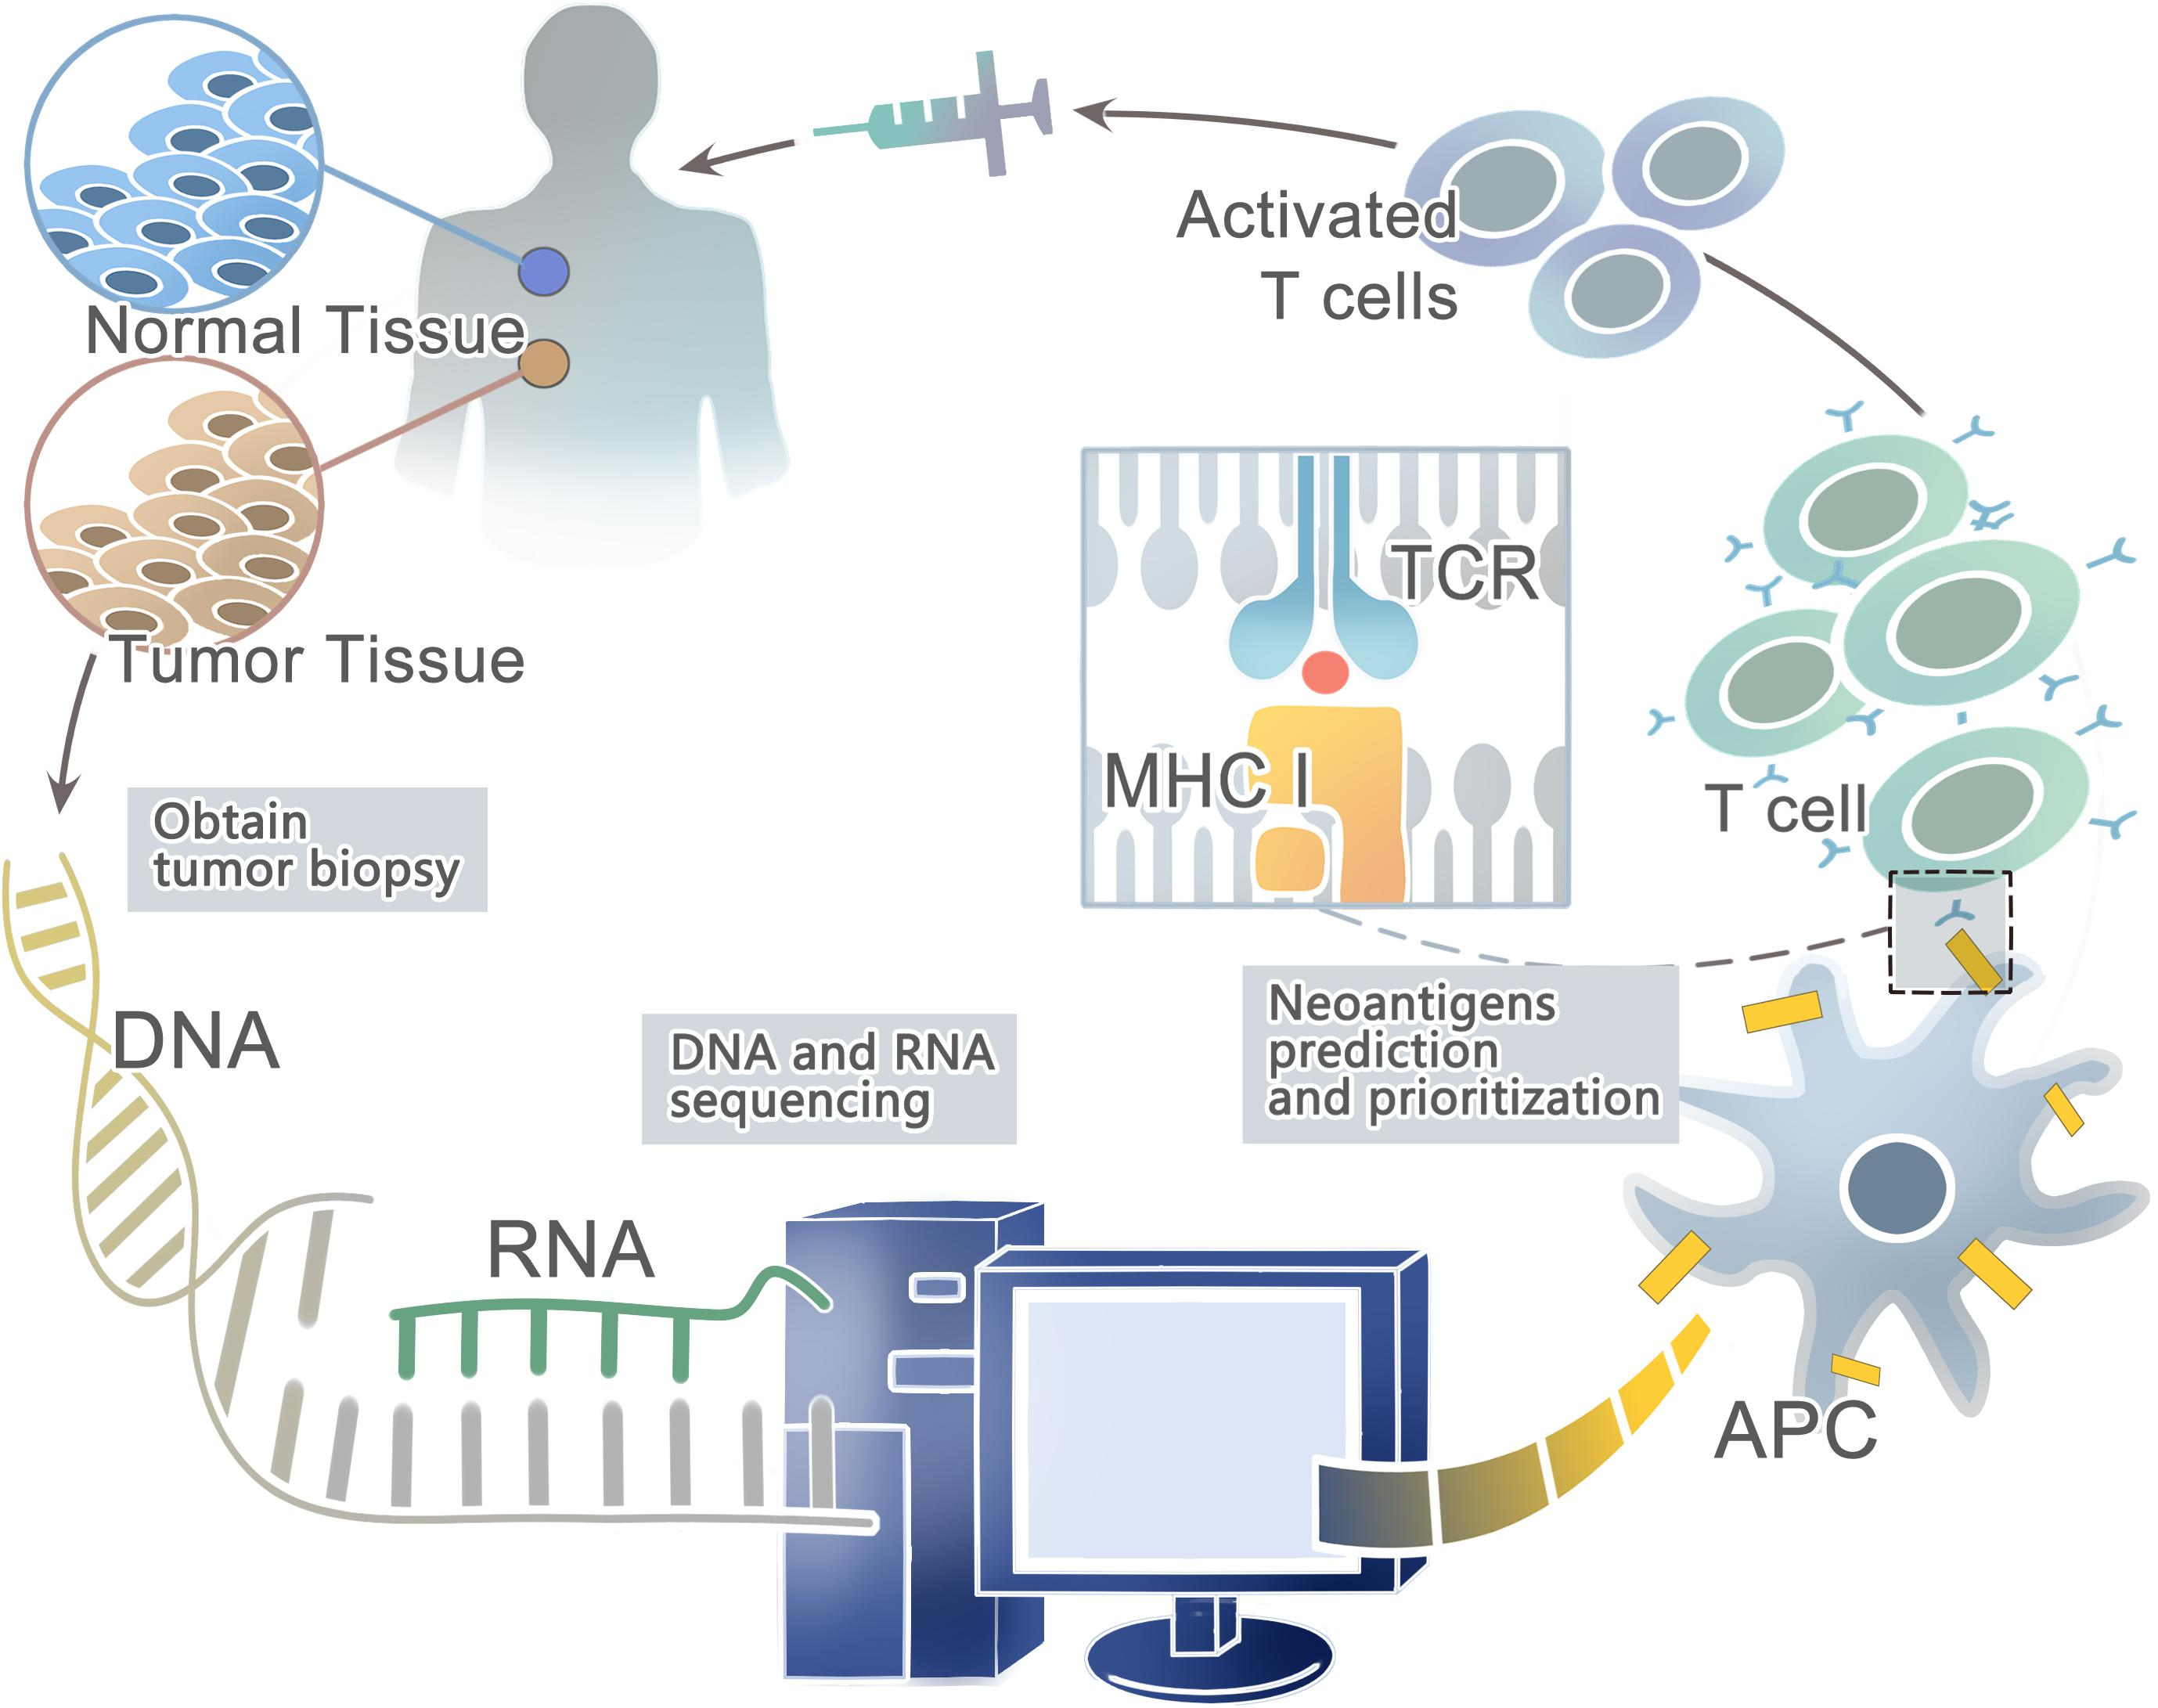
\includegraphics[width=0.45\textwidth]{../img/pipeline/vaccine_pipeline}}		
	\subfigure[Pipeline]{\label{fig:vaccines_b}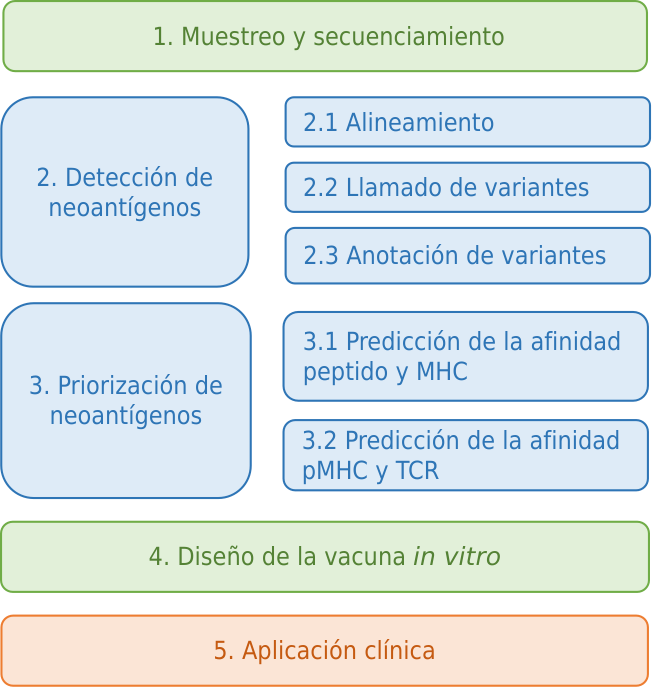
\includegraphics[width=0.45\textwidth]{img/pipeline/pipeline_spanish}}
	
	\caption[\textit{Pipeline} para el desarrollo de vacunas basadas en neoantígenos]{Marco de desarrollo para la creación de vacunas personalizadas contra el cáncer basadas en neoantígenos. (a) proporciona una visión general de cada etapa \citep{han2020progress}. (b) una visión general de cada fase con un énfasis en el desarrollo \textit{in-silico}.}
	\label{fig:vaccines}
\end{figure}

\section{Problema}
\label{sec:problema}

Los neoantígenos son peṕtidos mutados específicos de tumores y son considerados los principales causantes de una respuesta inmune \citep{borden2022cancer, chen2021challenges, gopanenko2020main}. Es así que surgen varios esfuerzos e investigación en la Inmunoterapia del cáncer, concentradas en el estudio y detección de neoantígenos. Es así, que el desarrollo de vacunas personalizadas basadas en neoantígenos es considerado uno de los métodos con mayor probabilidad de éxito \citep{borden2022cancer}. Incluso varias compañías como BioNTech, Genocea Biosciences, Neon Therapeutics y Gritstone Oncology realizan investigación y ofrecen el servicio de generar vacunas personalizadas a pacientes de cáncer.

Además, el MHC representa un factor clave, en la detección de neoantígenos, al ser el encargado de unirse al neoantígeno y presentarlo a la superficie de la célula. Debido a esto, este trabajo en enfoca en el desarrollo de un método para la predicción del enlace entre neoantígenos y MHC (\textit{pMHC binding}), esto corresponde a la Fase 3.1 de la Figura \ref{fig:vaccines}(b) dentro del \textit{pipeline} de detección de neoantígenos.  Existen dos tipos: el MHC clase I (MHC-I) y MHC clase II (MHC-II), ambos presentan péptidos en la superficie celular a las células T CD8+ y CD4+, respectivamente \citep{janeway1997immunobiology, abualrous2021major}. En detalle, el ciclo de vida de los neoantígenos que se unen a MHC-I se puede resumir de la siguiente manera. Primero, una proteína cancerígena se degrada en péptidos en el citoplasma. Luego, los péptidos se unen al MHC (\textit{pMHC binding}). Después, este compuesto sigue un camino hasta llegar a la membrana celular (\textit{pMHC presentation}). Finalmente, el pMHC es reconocido por el TCR, desencadenando el sistema inmunológico \citep{janeway1997immunobiology, wieczorek2017major, gasser2021interpreting}. Por lo tanto, la unión pMHC es un paso muy importante para la inmunidad celular, y la predicción y comprensión de esta unión tienen un valioso potencial. Lamentablemente, la mayoría de las ligandos pMHC no llegan a la membrana celular \citep{de2020neoantigen}. 

Adicionalmente, las proteínas MHC están codificadas por genes altamente polimórficos, llamados \textit{Antígenos Leucocitarios Humanos} (HLA); la considerable naturaleza polimórfica de los genes MHC proporciona una variación sustancial en la unión con los neoantígenos, lo que influye en el conjunto de neoantígenos presentados a las células T \citep{abualrous2021major}. En consecuencia, los métodos propuestos se categorizan como \textit{pan-specific} y \textit{allele-specific}. Los métodos \textit{allele-specific} \citep{rammensee1999syfpeithi, reche2002prediction, kim2009derivation, nielsen2016netmhcpan, vang2017hla, shao2020high, bravi2021rbm} entrenan un modelo para cada \textit{allele} del MHC; mientras que los métodos \textit{pan-specific} \citep{hu2019acme, liu2019deepseqpan, wu2019deephlapan, phloyphisut2019mhcseqnet, o2018mhcflurry, o2020mhcflurry, reynisson2020netmhcpan, venkatesh2020mhcattnnet, ye2021mathla, mei2021anthem, chu2022transformer, zhang2022hlab, mei2021anthem, hu2019acme, gfeller2023improved} entrenan un modelo global que toma péptidos (neoantígenos) y MHC como entradas. Además, la naturaleza polimórfica del MHC eleva bastante la complejidad de este problema, se cree que existen las 10000 diferentes MHC \textit{alleles} \citep{abelin2017mass}, esto complica mucho la detección de neo antígenos. Por lo tanto, los métodos \textit{pan-specific} surgen con una alta posibilidad de futuras aplicaciones.

Lamentablemente, a pesar de varios esfuerzos en el desarrollo  de métodos para la detección de neoantígenos, menos del 5\% de neoantígenos detectados activan el sistema immune \citep{de2020neoantigen, mill2022neoms, bulik2019deep, bassani2015mass, yadav2014predicting}. Según los autores de los métodos,  las razones son: 

\begin{enumerate}
	\item La no inclusión en conjunto de varias fuentes de información como DNA-seq, RNA-seq, y datos de \textit{Mass Spectrometry} (MS) \citep{kim2018neopepsee}. Por ejemplo, la mayoria de  propuestas no utiliza datos de MS; en la actualidad, existe una creciente información de estos datos y se estan aplicado a varios campos de la Bioinformática.
	\item  Uso herramientas de bajo desempeño para la predicción del enlace péptido-MHC (pMHC) (etapa 3.1  de la Figura \ref{fig:vaccines_b}). La mayoria de aplicaciones, se basa en el uso de MHCFlurry \citep{o2020mhcflurry} y NetMHCpan4.1 \citep{reynisson2020netmhcpan}. Sin embargo, actualmente, se cuenta con herramientas de mejor desempeño basado en \textit{Transformers} \citep{arceda2023neoantigen}. Esta tésis, se enfoca en resolver este problema.
	\item Para la etapa 3.2 de la Figura \ref{fig:vaccines_b}, los autores no consideran  la predicción del enlace pMHC al TCR (pMHC-TCR), varios autores consideran incluir esta tarea en trabajos futuros  \citep{rubinsteyn2018computational}.
	\item Finalmente, no utilizar información de eventos de \textit{alternative splicing}, variaciones estructurales en el ADN y las mutaciones de fusión de genes, está información esta fuertemente relacionada con varios tipos de cancer \citep{wood2020neoepiscope}.
\end{enumerate}

En conclusión, la detección de neoantígenos es un desafío que consta de múltiples etapas, y las herramientas actuales en el estado del arte presentan un rendimiento insuficiente. Uno de los factores clave detrás de este bajo rendimiento está relacionado con la predicción del enlace pMHC. Por esta razón, esta tésis se centra en abordar este problema mediante la propuesta de un método basado en \textit{Transformers} para la predicción del enlace/unión pMHC.

%Finalmente, la detección de neoantígenos es un problema compuesto por varias etapas, y las herramientas actuales del estado del arte tiene bajo desempeño. Además, una de las principales razones del bajo desempeño esta relacionado a la predicción del enlace pMHC. Debido a eso, esta tesis, se enfoca en dar solución a este problema, proponiendo un método basado en Transformers para la predicción del enlace pMHC.

%Según lo mencionado anteriormente, la detección de neo antígenos es un factor clave en el desarrollo de vacunas personalizadas. En este proceso el compuesto \textit{Major Histocompatibility Complex} (MHC), juega un papel muy importante, es el encargado de presentar los péptidos a la células T \citep{hashemi2022improved}. Para el caso de células humanas el gen MHC es conocido como Human Leukocyte Antigens (HLA) y es polimórfico, se cree que existen las 10000 diferentes \textit{HLA-I alleles} \citep{abelin2017mass}, esto complica mucho más la detección de neo antígenos. 

%El ciclo de vida de un neo antígeno para células con núcleo podría resumirse como: primero una proteína es degradada en péptidos en el citoplasma de las células, luego los péptidos se enlazan a la molecula MHC (\textit{pMHC binding}), luego este compuesto sigue un trayecto hasta llegar a la membrana de la célula (\textit{pMHC presentation}), finalmente el compuesto pMHC es reconocido por  el T-cell Receptor (TCR) de las células T y así si activaría el sistema inmune. Además, el número de posibles péptidos enlazables a MHC  son entre 1000 a 10000, esto es el 0.1\% de los posibles péptidos  de 9 aminoacidos\footnote{La mayoría de péptidos enlazados a moléculas MHC-I tienen 9 aminoácidos, se suele utilizar el termino \textit{n-mer} para referirse a péptidos de \textit{n} aminoácidos.} \citep{abelin2017mass}. En este proceso, el objetivo es detectar los péptidos (neo antígenos) que llegan a la membrana de la célula, luego con ayuda de procedimientos de biotecnología, se entrena a las células T de un paciente para que aprenda a reconocer los neo antígenos.


%El problema de \textit{pMHC binding} está casi solucionado con una precisión de 0.98 por parte de la herramienta NetMHCPan 4.1 \citep{reynisson2020netmhcpan}. Sin embargo, no es bueno limitar la detección de neo antígenos solo al problema de \textit{pMHC binding}, porque la mayoría de estos compuestos no llegan a la membrana \citep{mill2022neoms}, a este problema se le conoce como \textit{pMHC presentation}. Por ejemplo, se sabe que menos del 5\% de péptidos detectados llegan a la membrana \citep{de2020neoantigen, mill2022neoms, bulik2019deep, bassani2015mass, yadav2014predicting}. Además, existen herramientas como NeyMHC, NetMHCpan y MHCFlurry que tienen un buen desemepeño en \textit{pMHC binding}, pero con resultados pobres en  \textit{pMHC presentation} \citep{bulik2019deep}. 



\subsection{Formulación del Problema}

El presente estudio se centra en el problema de predicción del enlace pMHC-I (\textit{pMHC binding prediction}). Esto representa un problema de clasificación binaria que toma como entrada la secuencia de aminoacidos de un péptido y el MHC. Un péptido podría representarse como: $p = \{A, ..., Q\}$ y una representación similar para el MHC sería: $q = \{A, N, ..., G\}$. Finalmente, necesitamos conocer la probabilidad de afinidad entre $p$ y $q$. Si esta probabilidad es lo suficientemente alta, es posible que el péptido se enlace al MHC y por lo tanto, el péptido $p$ en cuestión, sería un excelente candidato a neoantígeno.


%Menos del 5\% de péptidos detectados en \textit{pMHC binding}, llegan a la membrana de la células, para que luego sean reconocidos por las células T.  El proceso por el cúal un péptido enlazado a MHC llegue a la membrana es conocido como  \textit{pMHC presentation}, pero en este problema las propuestas recientes solo llegan a un 0.61 de precisión y 0.4 de \textit{recall}. Además, propuestas recientes solo llegan aun 0.6 de \textit{presicion} y 0.4 de \textit{recall} \citep{mill2022neoms}. En este contexto, la tesis se enfoca en el problema de \textit{pMHC presentation}, considerándolo como un problema de clasificación binaria, y tomando como entrada la secuencia de aminoácidos del péptido y la secuencia de aminoácidos de la proteína MHC. 



%% ------------------------------------------------------------------- %%
\section{Objetivos}
\label{sec:objetivos}

\subsection{Objetivo General}

%Detección \textit{in Silico} de Neoantígenos Utilizando \textit{Transformers} y \textit{Transfer Learning} en el Marco de Desarrollo de Vacunas Personalizadas para Tratar el Cáncer

Implementar un método \textit{in silico} basado en \textit{Transformers} y \textit{Transfer Learning} para la detección de neoantígenos, enfocados en la predicción de la unión pMHC. 

\subsection{Objetivos Específicos}

\begin{enumerate}[(a)]
	%\item Analizar herramientas del estado del arte como: NetMHCpan4.1, MHCFlurry2.0, Anthem, ACME y MixMHCpred2.2, utilizadas para la predicción del enlace pMHC en el contexto de detección de neonatígenos.
	\item Analizar los métodos que utilizan \textit{Transformers} para la predicción del enlace pMHC en el contexto de detección de neoantígenos.
	\item Analizar los modelos basados en \textit{Transformers} TAPE, ProtBert-BFD, y EMS2 pre-entredados para diversas tareas en Proteómica y de los cuáles se puede aplicar \textit{Transfer Learning}. 	
	\item Implementar \textit{fine-tuning} a los modelos TAPE, ProtBert-BFD, y EMS2 para la tarea de predicción del enlace pMHC, aplicando \textit{Gradient Accumulation Steps} (GAS) y una metodología de congelamiento de capas.
	\item Comparar los modelos de mejor desempeño con las herramientas del estado del arte como: NetMHCpan4.1, MHCFlurry2.0, Anthem, ACME y MixMHCpred2.2.
%\item Realizar una revisión sistemática de la literatura e implementar los métodos con mejor desempeño en la detección de neo antígenos.
%\item Proponer e implementar un método basado en \textit{deep learning} para la detección de neo antígenos.		
%\item Evaluar el método propuesto en bases de datos publicas.
\end{enumerate}

%% ------------------------------------------------------------------- %%
\section{Contribuciones}
\label{sec:contribuciones}
Las principales contribuciones de este trabajo son:

\begin{enumerate}[(a)]
	\item Desarrollo de  una revisión sistemática de la literatura referente a los métodos basados en \textit{Transformers} para la detección de neoantígenos. Se cuenta con dos publicaciones: \textit{``Deep Learning and Transformers in MHC-Peptide Binding and Presentation Towards Personalized Vaccines in Cancer Immunology: A Brief Review''} \citep{machaca2023deep} y \textit{``Transformers Meets Neoantigen Detection: A Systematic Literature Review''}.
	\item \textit{Fine-tuning} a seis modelos de \textit{Transformers} para la predicción del enlace pMHC; además, se ha evaluado el uso de GAS y una metodología de congelamiento de capas. Se cuenta con dos publicaciones: \textit{``Neoantigen Detection Using Transformers and Transfer Learning in the Cancer Immunology Context''} \citep{arceda2023neoantigen} y \textit{``Fine-tuning Transformers for Peptide-MHC Class I Binding Prediction''}.
	\item Comparación de los métodos propuestos con herramientas del estado del arte como: NetMHCpan4.1, MHCFlurry2.0, Anthem, ACME y MixMHCpred2.2. Los métodos propuestos tienen los mejores resultados en \textit{accuracy}, \textit{Area Under the Curve} (AUC), \textit{recall}, \textit{f1-score} y \textit{Matthews Correlation Coefficient}  (MCC).
\end{enumerate}

\clearpage
%% ------------------------------------------------------------------- %%
\section{Organización del Trabajo}
\label{sec:organizaciondeltrabajo}

El restante de este trabajo está organizado de la siguiente manera:

\begin{itemize}
	\item En el Capítulo \ref{cap:marcoteorico} se presentan los conceptos básicos sobre Bioinformática e inmunoterapia del Cáncer, también son abordados temas sobre \textit{Deep Learning} y redes neuronales \textit{Transformers}.
	
	\item Luego, en el Capítulo \ref{cap:estadodelarte} se describen los trabajos relacionados a la presente tésis. Debido a la gran cantidad de publicaciones, solo se ha considerado trabajos desde el 2018 y que hacen uso de \textit{Transformers} o redes reuronales con mecanismos de atención.
	
	\item El Capitulo \ref{cap:propuesta}, presenta la propuesta de la tésis. Esta se basa en un método para desarrollar \textit{fine-tuning} a \textit{Transformers} pre-entrenados para diversas tareas de Proteómica. 
	
	\item Luego, en el Capítulo  \ref{cap:resultados}, se presentan los resultados de la investigación. Además, se presenta una comparación con los métodos del estado del arte.
	
	\item Finalmente, en el Capítulo~\ref{cap:conclusiones} son expuestos las conclusiones del presente trabajo así como también las direcciones para continuar con el mismo en la sección de trabajos futuros.
	
	
	
\end{itemize}





%Em anexos está uma exemplificação da especificação da arquitetura, 
%neste caso é descrita a especificação da arquitetura 
%DAS-3 (Apêndice \ref{ape:especificacoes}).


%%%%%
 % Introduction
%% ------------------------------------------------------------------- %%
%% ------------------------------------------------------------------- %%
%% ------------------------------------------------------------------- %%
%% ------------------------------------------------------------------- %%
\chapter{Marco Conceptual}
\label{cap:marcoteorico}

\lhead{\emph{Marco Conceptual}} 

El proyecto pertenece al área de Bioinformática y específicamente a la Inmunoinformática, en este contexto el marco teórico detalla conceptos de Biología Molecular (ADN, ARN y proteínas), Inmunología y Ciencias de la Computación. 

\section{Bioinformática y Biología Molecular }

En esta sección, describiremos los principales conceptos referentes a Biología Molecular que serán considerados en la propuesta de la tesis.

\subsection{Bioinformática}

Según \cite{luscombe2001bioinformatics}, la Bioinformática involucra la tecnología que utiliza las computadoras para el almacenamiento, manipulación y distribución de información relacionada a la Biología Molecular como DNA, RNA y proteínas. También podemos considerar que la Bioinformática se enfoca al análisis de secuencias, estructuras y funciones de los genes y proteínas; algunas veces también puede ser llamado Computación Molecular Biológica \citep{xiong2006essential}.


\subsubsection{DNA, RNA y Proteínas}

\textit{Deoxyribonucleic Acid} (DNA) es una molécula dentro de las células que contiene información genética responsable del desarrollo y función del organismo \citep{NCIdictionary2022}. Gran parte del DNA se sitúa dentro del núcleo de las células (en organismos Eucariotes). Por ejemplo en la Figura \ref{img:dnalocation}, vemos como el DNA, forma parte de los cromosomas y estos a su vez están en el núcleo. Luego, podemos notar, que los genes representan segmentos del DNA. Finalmente, en la Figura \ref{img:dnalocation}, notamos las bases nitrogenadas que componen el DNA: \textit{Guanine}, \textit{Cytosine}, \textit{Adenine} y \textit{Thymine}; normalmente, estas bases serán representadas por las letras: G, C, A, T respectivamente.

\begin{figure}[H]
	\centering
	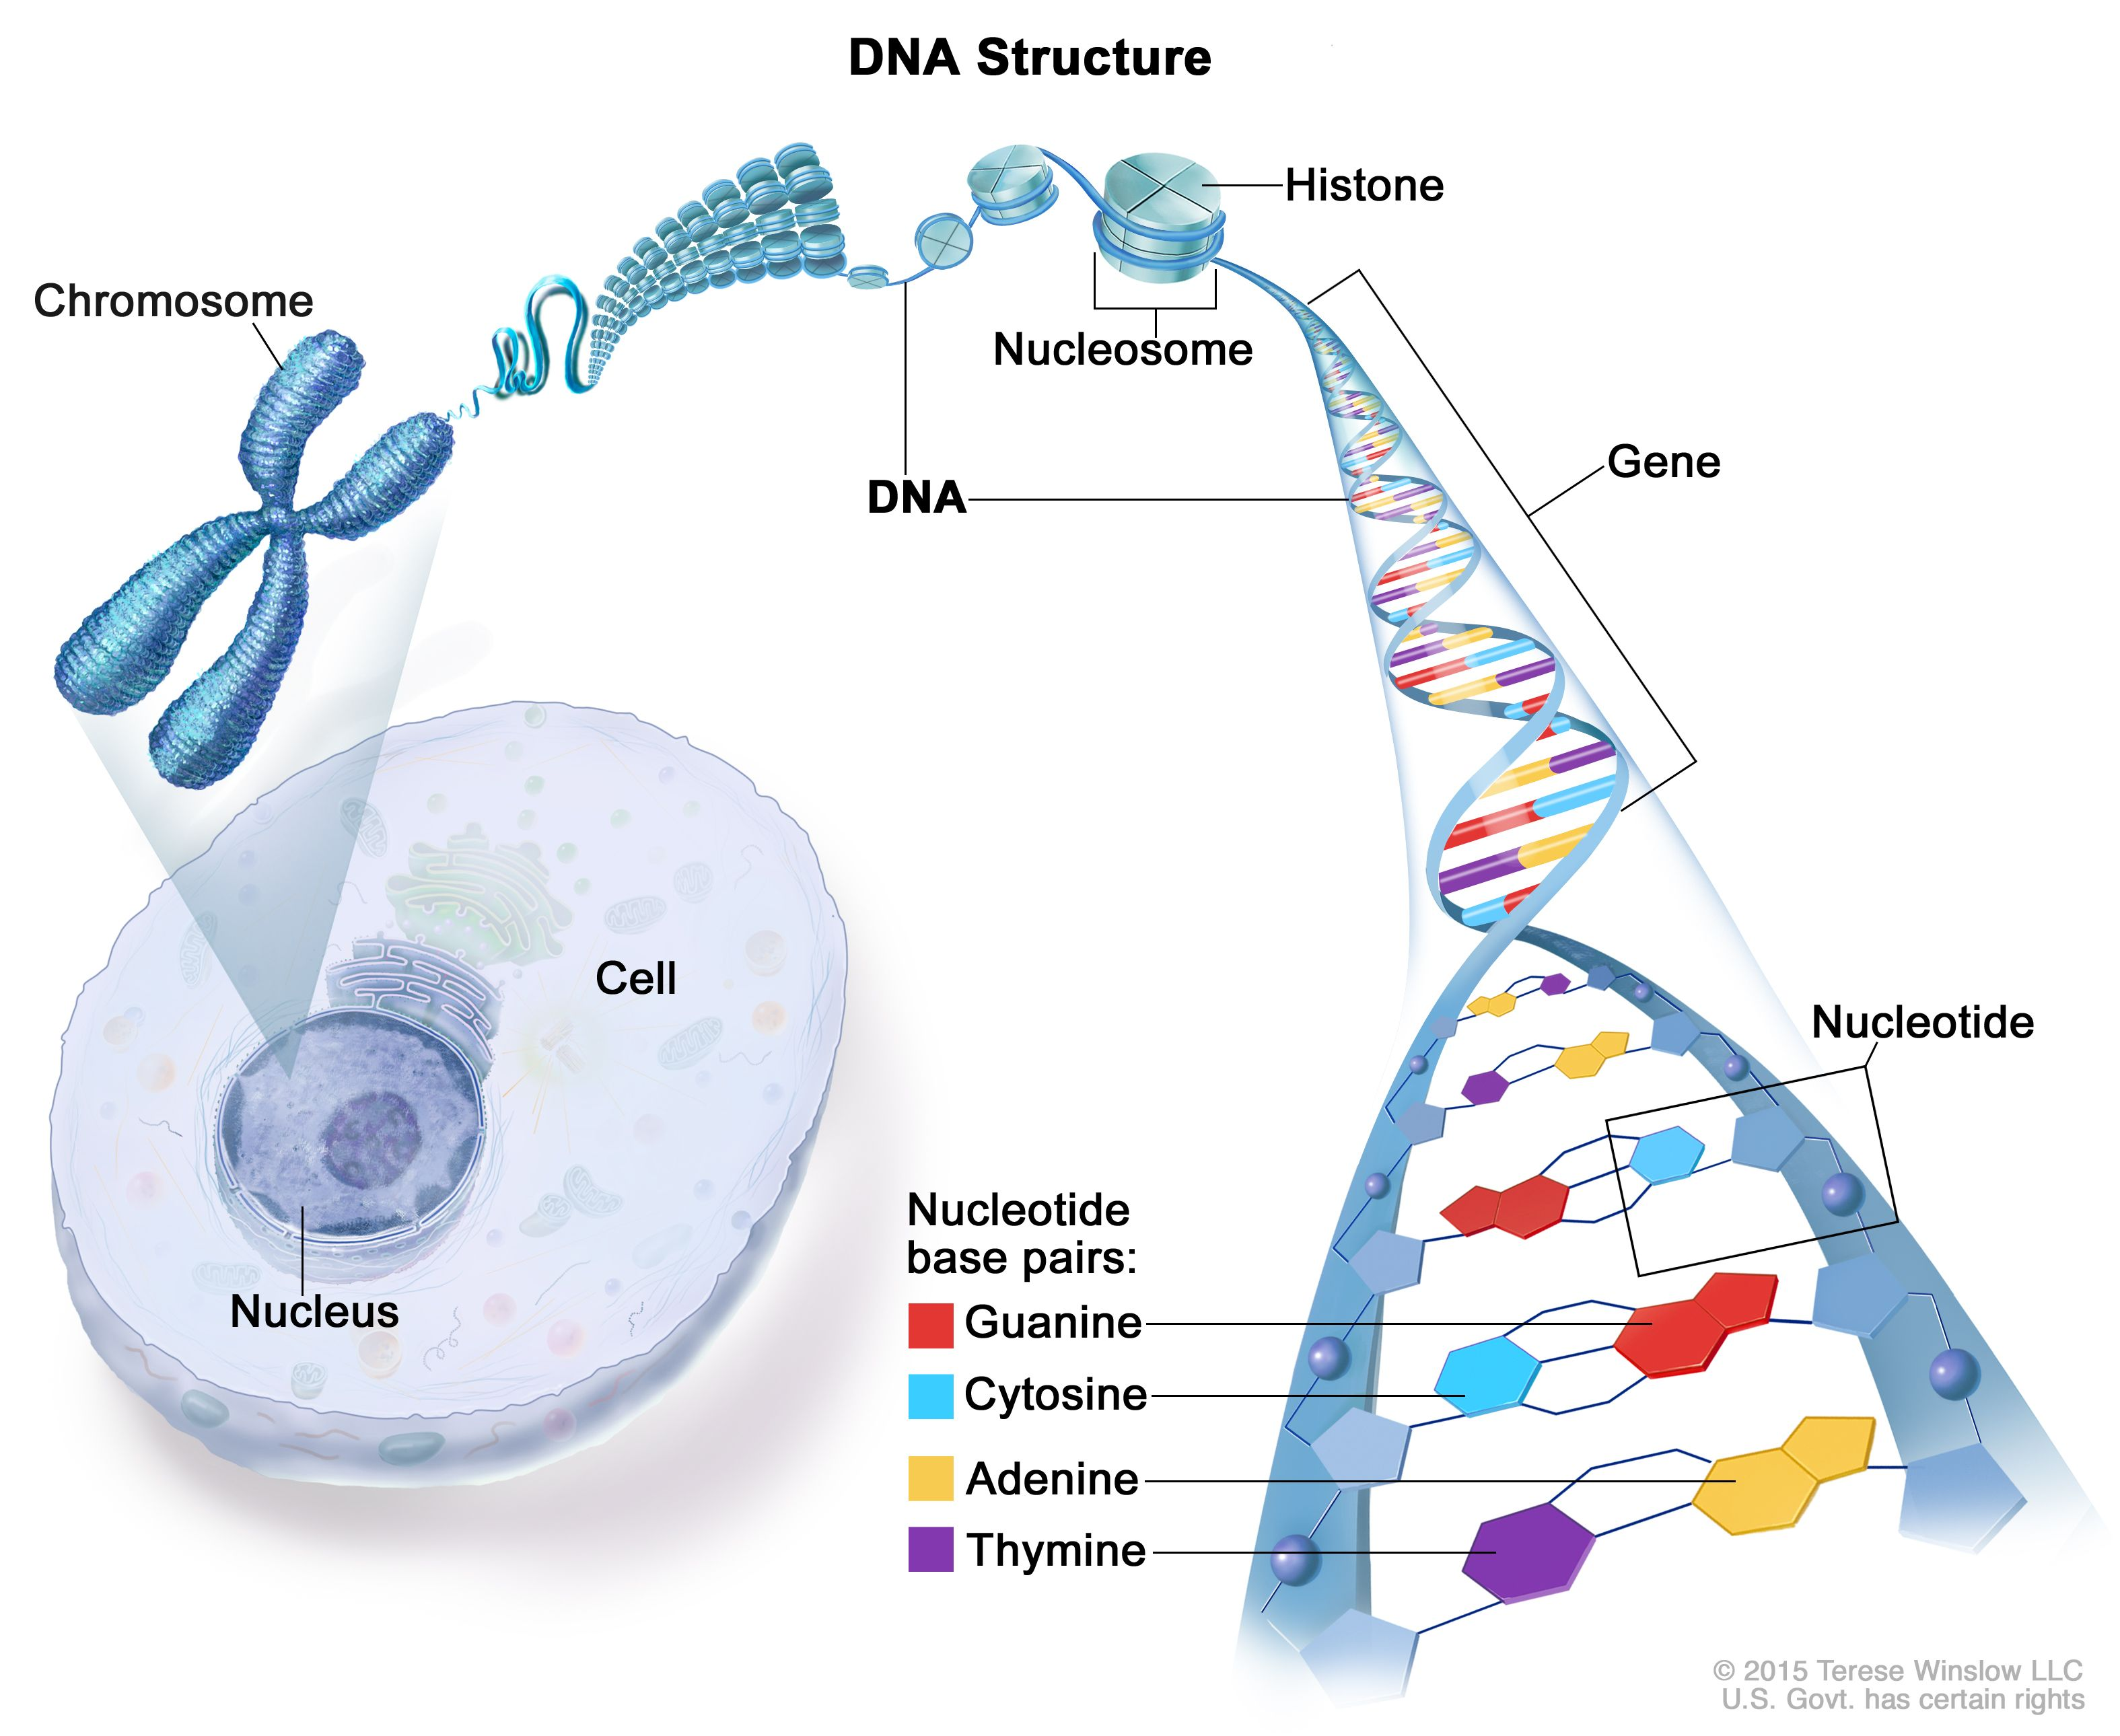
\includegraphics[width=0.6\textwidth]{img/neoantigen/dna}
	\caption{Localización y estructura del DNA. Fuente:  \cite{NCIdictionary2022}.}	
	\label{img:dnalocation}
\end{figure}

Durante el ciclo de vida de la célula, ocurre un proceso llamado Transcripción (ver Figura \ref{img:trans}), en este proceso se generan cadenas de \textit{Ribonucleic Acid} (RNA) a partir de la cadena de DNA \citep{NCIdictionary2022}.  Durante este proceso la base nitrogenada \textit{Thymine} (T) es reemplazada por \textit{Uracil} (U). El proceso mencionado, ocurre dentro del núcleo de la célula y en esta etapa el RNA es llamado \textit{messenger RNA} (mRNA). Una vez el mRNA sale del núcleo, es transportado por \textit{transfer RNA} (tRNA) hacia los Ribosomas (ver Figura \ref{img:trans}). En está, última etapa ocurre la Traducción, cada grupo de tres bases nitrogenadas (codones) se convierten en un aminoácido diferente, luego estos aminoácidos forman cadenas polipeptídicas y estas a su vez forman las proteínas; normalmente, cada gen genera una proteína \citep{xiong2006essential, NCIdictionary2022}.



\begin{figure}[H]
	\centering
	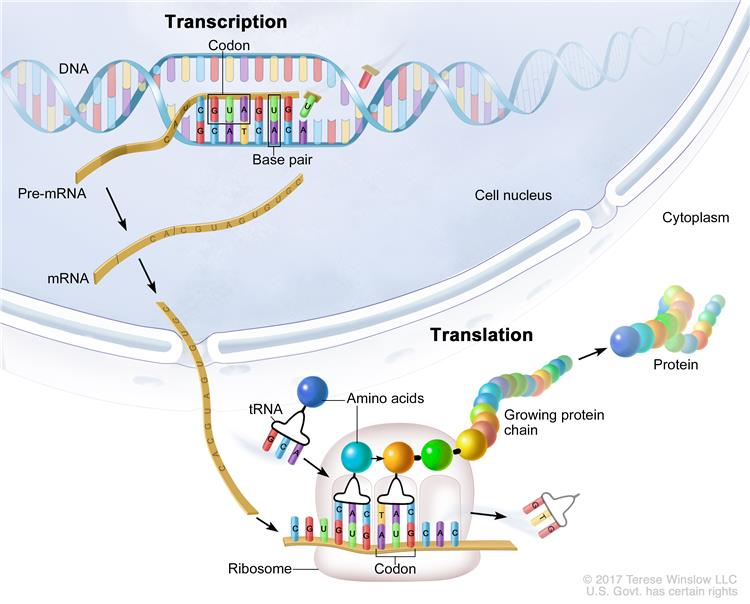
\includegraphics[width=0.7\textwidth]{img/neoantigen/trans}
	\caption{Transcripción y traducción. Fuente:  \cite{nci2020}.}	
	\label{img:trans}
\end{figure}

Durante el proceso de Traducción, puede ocurrir un fenómeno llamado \textit{Alternative Splicing}. Por ejemplo , en la Figura \ref{img:alt}, notamos como un gen puede generar tres proteínas distintas, cada una con funciones distintas. Este fenómenos, complica bastante el análisis de DNA.


\begin{figure}[H]
	\centering
	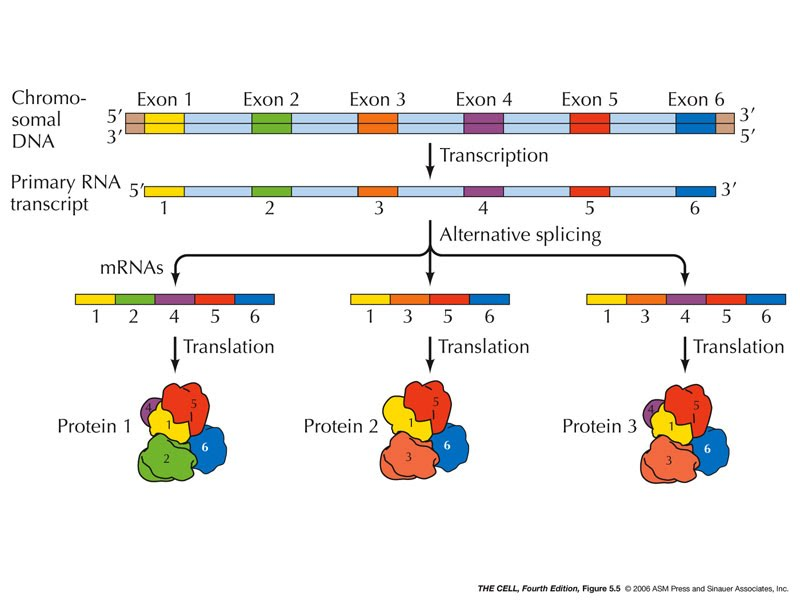
\includegraphics[width=0.7\textwidth]{img/neoantigen/alt}
	\caption{\textit{Alternative Splicing}. Fuente:  \cite{nci2020}.}	
	\label{img:alt}
\end{figure}


\subsection{Mutaciones}

Las mutaciones también llamadas variaciones, representan cualquier cambio en la secuencia de DNA, estos pueden ocurrir durante la división celular o por la exposición a agentes químicos o radioactivos. Estas mutaciones pueden ser beneficiosas, dañinas (cuando afectan la generación de proteínas) o no tener algún efecto  \citep{NCIdictionary2022}. Varios tipos de Cáncer son ocasionados por estas mutaciones \citep{borden2022cancer, chen2021challenges, de2020neoantigen}. \\ 

Según el tipo de célula afectada, tenemos: mutaciones somáticas y mutaciones \textit{germline} (una mutación en estas células puede ser heredada a la descendencia) \citep{clancy2008genetic}.  Según \citep{xu2018review}, las variaciones genómicas pueden clasificarse en tres grupos: \textit{Single-Nucleotide Variant} (SNV), inserciones y eliminaciones (INDELS) y \textit{Structural Variation} (SV). Una mutación se considera SNV cuando las variaciones afectan a menos de 10 bases. \\

En la Figura \ref{fig:SNV}, presentamos ejemplos de SNV. Por ejemplo, las sustituciones pueden afectar la generación de un aminoácido, pero las inserciones o eliminaciones pueden afectar en cadena la generación de varios aminoácidos, a este tipo de fenómeno se le conoce como \textit{frameshit mutation} \citep{xu2018review}.


\begin{figure}[h]
	\centering
	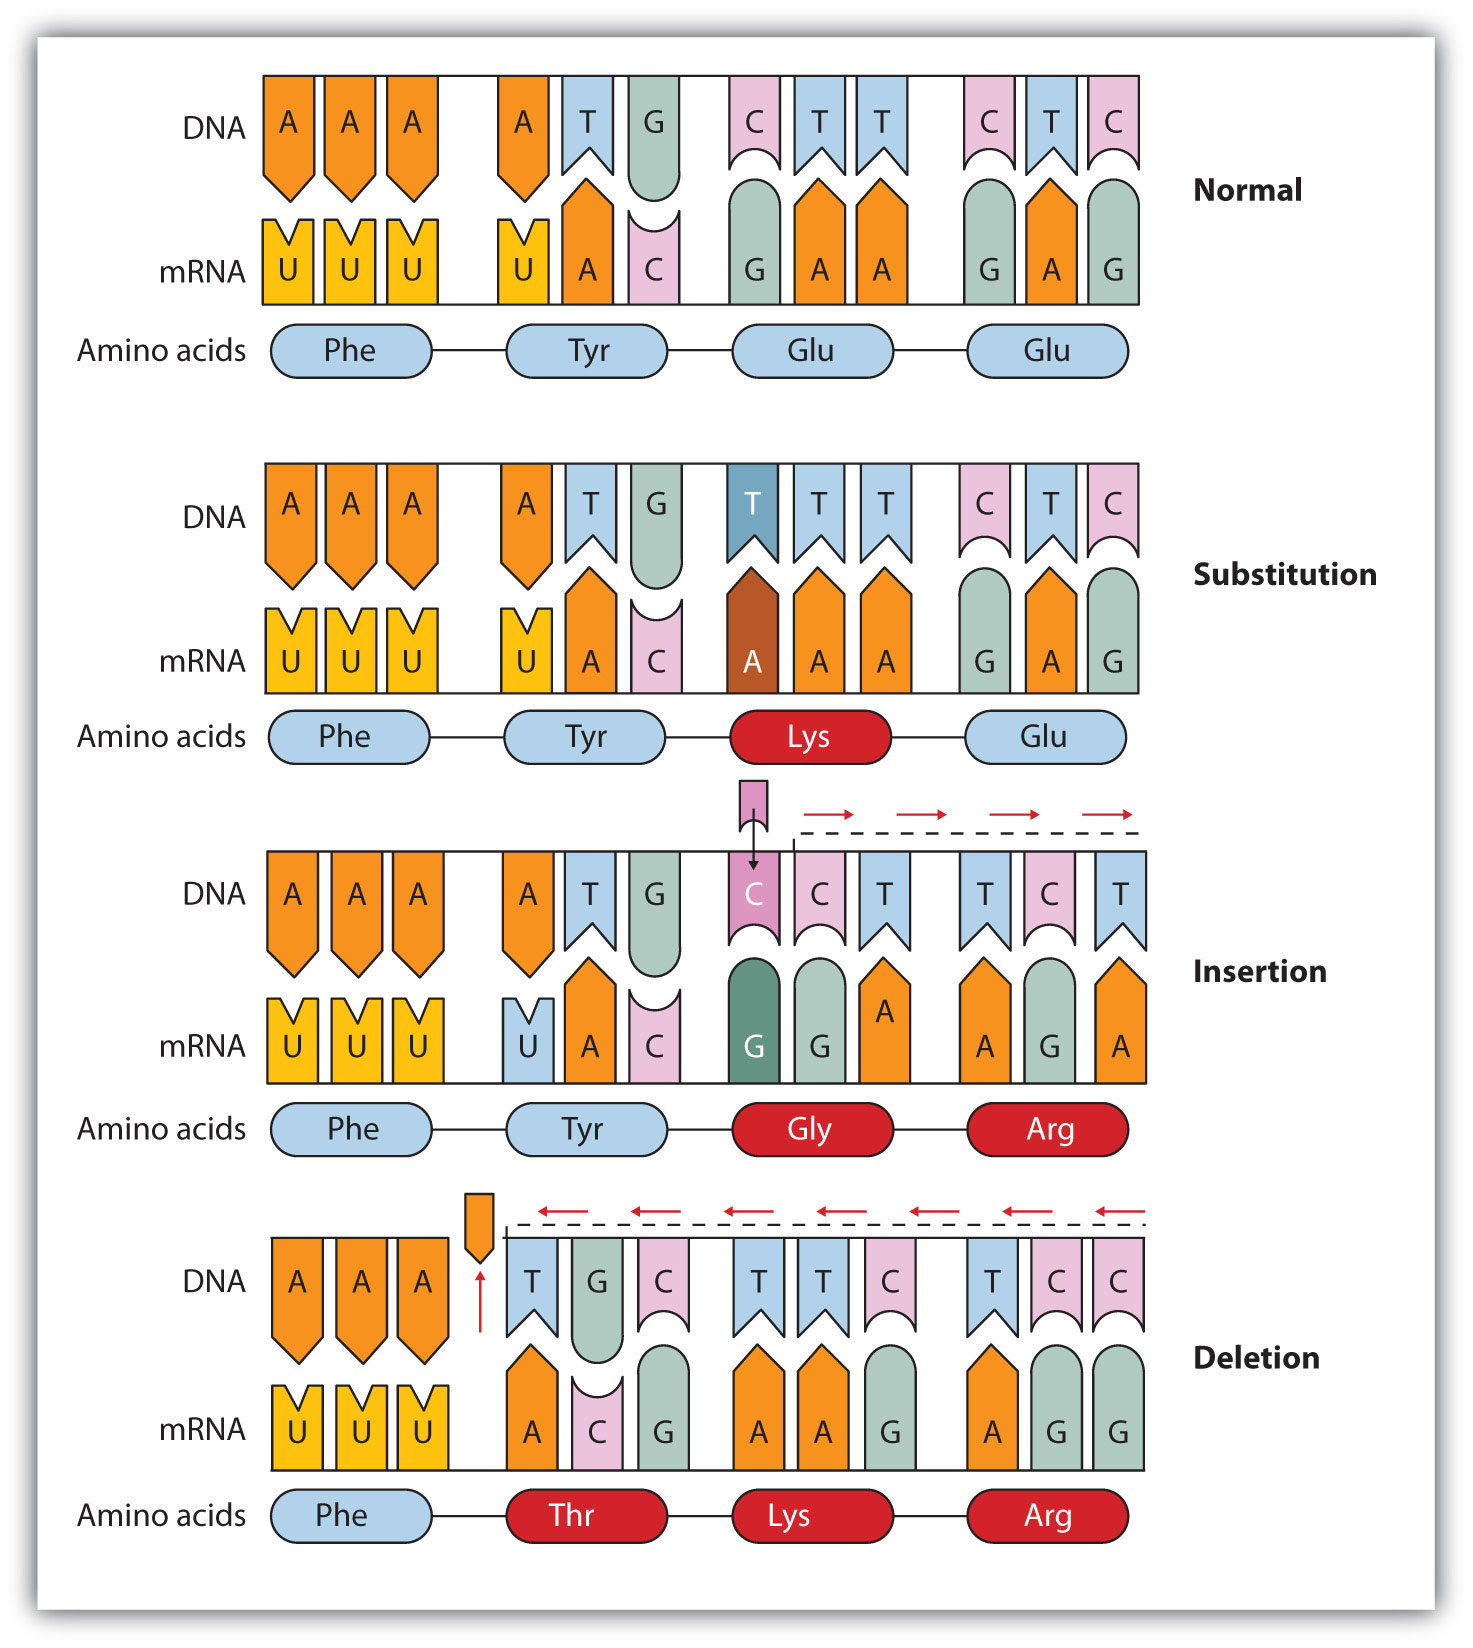
\includegraphics[width=0.6\textwidth]{img/neoantigen/SNV}
	\caption{Ejemplos de SNV en el DNA. Fuente: \cite{socrates2022}}
	\label{fig:SNV}
\end{figure}

En la Figura \ref{fig:variants}, mostramos algunos tipos de SV. En este caso, también se pueden presentar INDELS, \textit{Tanden duplication}, inversiones, traslocaciones y \textit{Copy Number Variants} (CNV). Los CNVs, representan fuertes candidatos para ser biomarcadores de varios tipos de Cáncer \citep{pan2019identification, lucito2007copy}. Otra mutación importante, es referente a la fusión de genes, en estos casos dos o más genes se fusionan y forman una proteína completamente diferente, este tipo de mutación también está fuertemente relacionado a varios tipos de Cáncer \citep{kerbs2022fusion, kim2019fusiongdb, heyer2020sequencing}.

\begin{figure}[h]
	\centering
	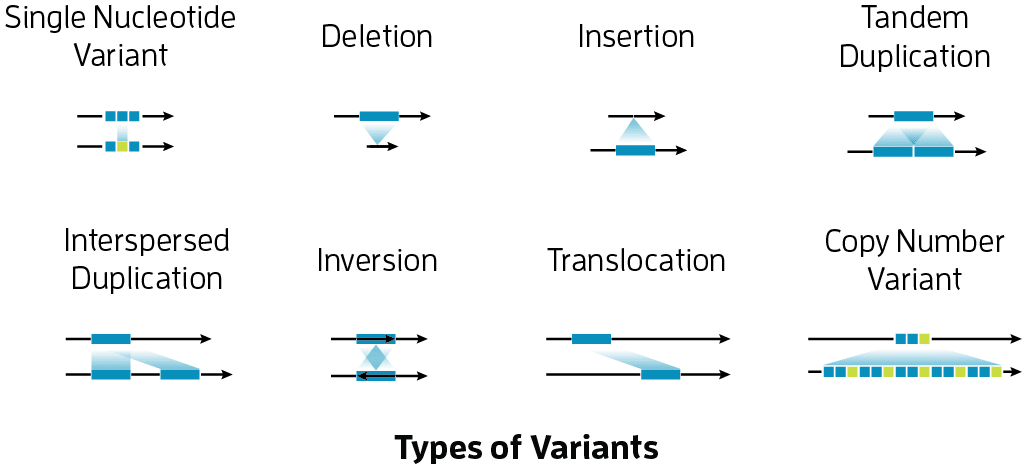
\includegraphics[width=0.6\textwidth]{img/neoantigen/variants}
	\caption{Ejemplos de variaciones en el DNA. Fuente: \cite{sv_pacbio_2021}}
	\label{fig:variants}
\end{figure}

\section{Sistema inmunitario}

El sistema inmunitario hace referencia al conjunto de células y procesos químicos que tiene como función protegernos de agentes extraños como: microbios, bacterias, células de Cáncer, toxinas, etc. \cite{marshall2018introduction}. En esta sección, se explicará de forma breve el comportamiento del sistema inmunitario frente cuando un agente extraño (antígeno) ingresa al cuerpo humano.

\subsection{Células T y APC}

Las células T también llamadas linfocitos T, se forman a partir de la médula ósea y son los encargados de eliminar agentes extraños (antígenos) \cite{NCIdictionary2022}. Estas células están compuestas por un T-cell Receptor (TCR), que es el encargado de reconocer y enlazar a los antígenos. Luego, algunas células T, requieren de la acción de los \textit{Antigen Presenting Cells} (APC), estás células APC son: células dentríticas, macrofagos, células B, fibroblastos y células epiteliales. Normalmente, los APC devoran los antígenos y luego los presentan a las células T para su eliminación  \citep{marshall2018introduction}.


\subsection{MHC I y II}

\textit{Major Histocompatibility Complex} (MHC) I y II, son proteínas que desempeñan un rol importante en el sistema inmunitario. Ambas proteínas tienen la función de presentar péptidos (antígenos) en la superficie de las células, para que sean reconocidas por la células T \citep{abualrous2021major}. MHC-I se encarga de la presentación de las células con núcleo, mientras que MHC-II, de las células APC. \\

El proceso de presentación de los antígenos por MHC-I es el siguiente (Figura \ref{fig:mhc1}): la proteína foránea es degradado por el proteasoma y se producen péptidos (posibles antígenos), luego estos péptidos son transportados al Endoplasmic Reticulum (ER) con la ayuda de \textit{Transporter associated Antigen Processing} (TAP), luego es migrado al aparato de Golgi para ser presentado en la superficie de la célula y es enlazado a la proteína MHC-I, una vez en la superficie, el antígeno puede ser reconocido por las células CD8+T \citep{zhang2019application}.




\begin{figure}[H]
	\centering
	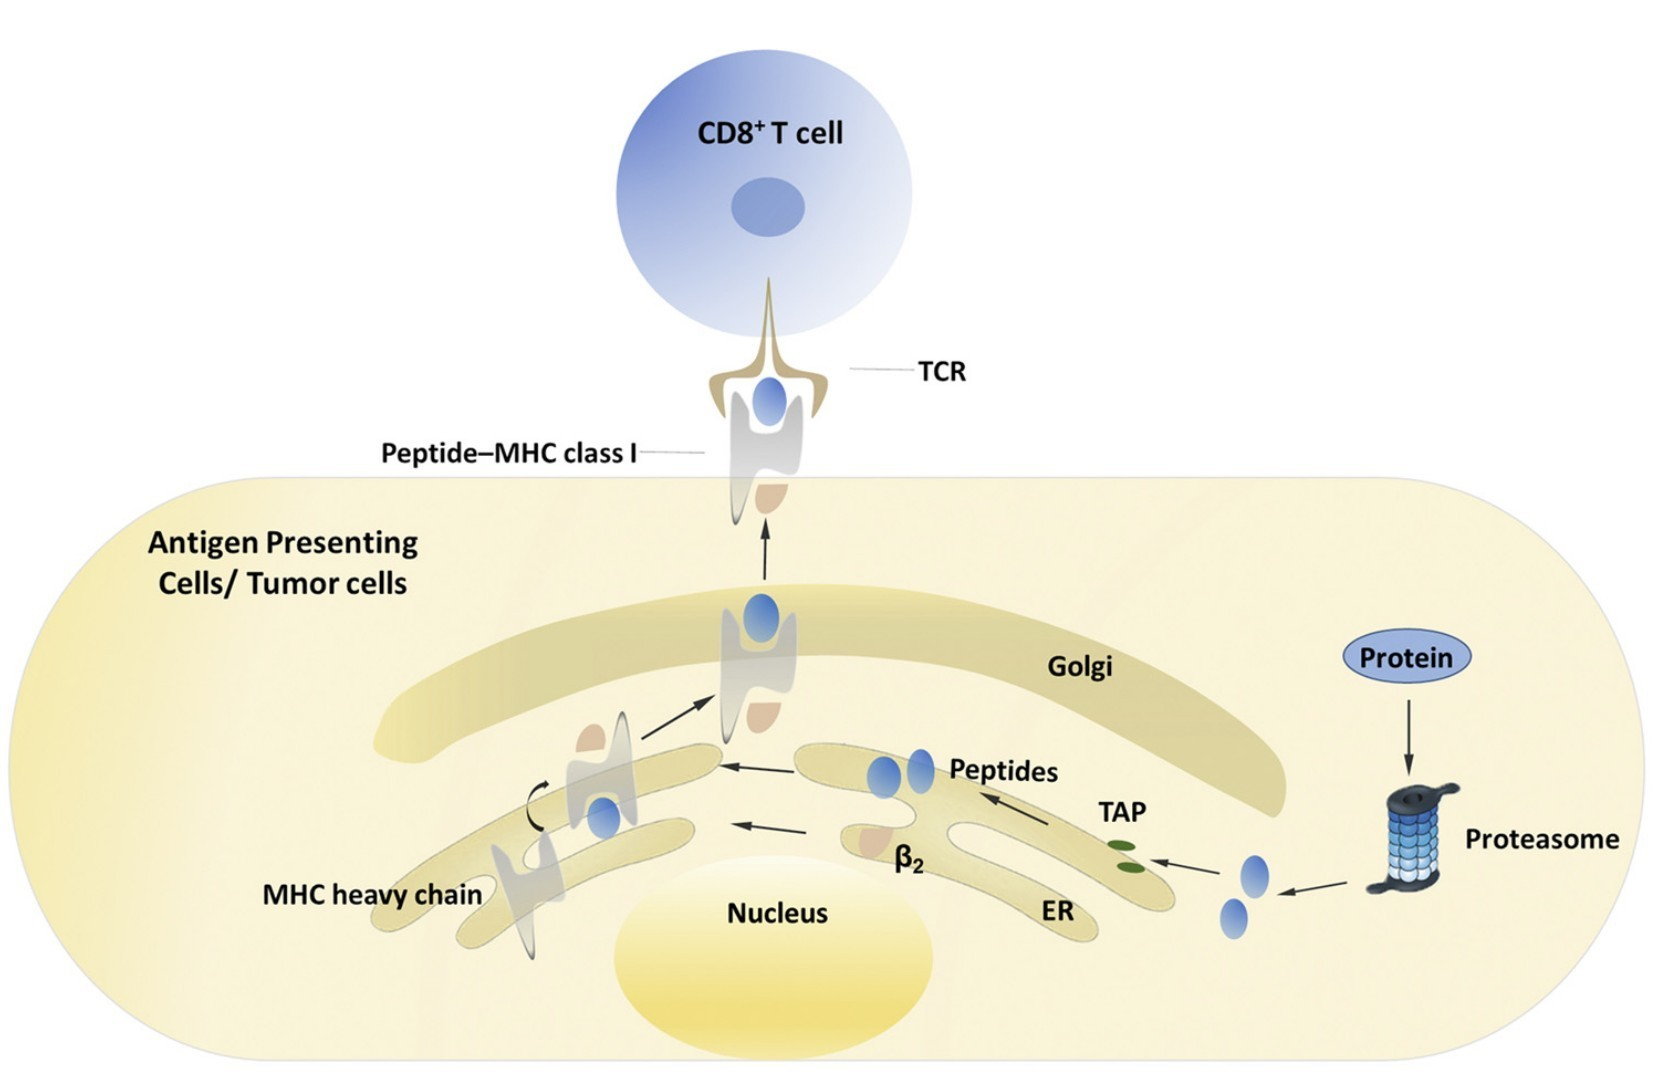
\includegraphics[width=0.8\textwidth]{img/neoantigen/mhc1.jpg}
	\caption{Presentación de antígenos por MHC-I. Fuente: \cite{zhang2019application}}
	\label{fig:mhc1}
\end{figure}

Para el caso de MHC-II, es un proceso similar (Figura \ref{fig:mhc2}): primero, los patógenos son devorados por fagocitosis, los péptidos asociados a MHC-II son producidos en el Endoplasmic Reticulum (ER), para luego ser trasladados al aparato de Golgi, y luego ser transportados a la superficie de las células una vez enlazadas con MHC-II, finalmente, son reconocidas por las células CD4+T \citep{zhang2019application}.



\begin{figure}[H]
	\centering
	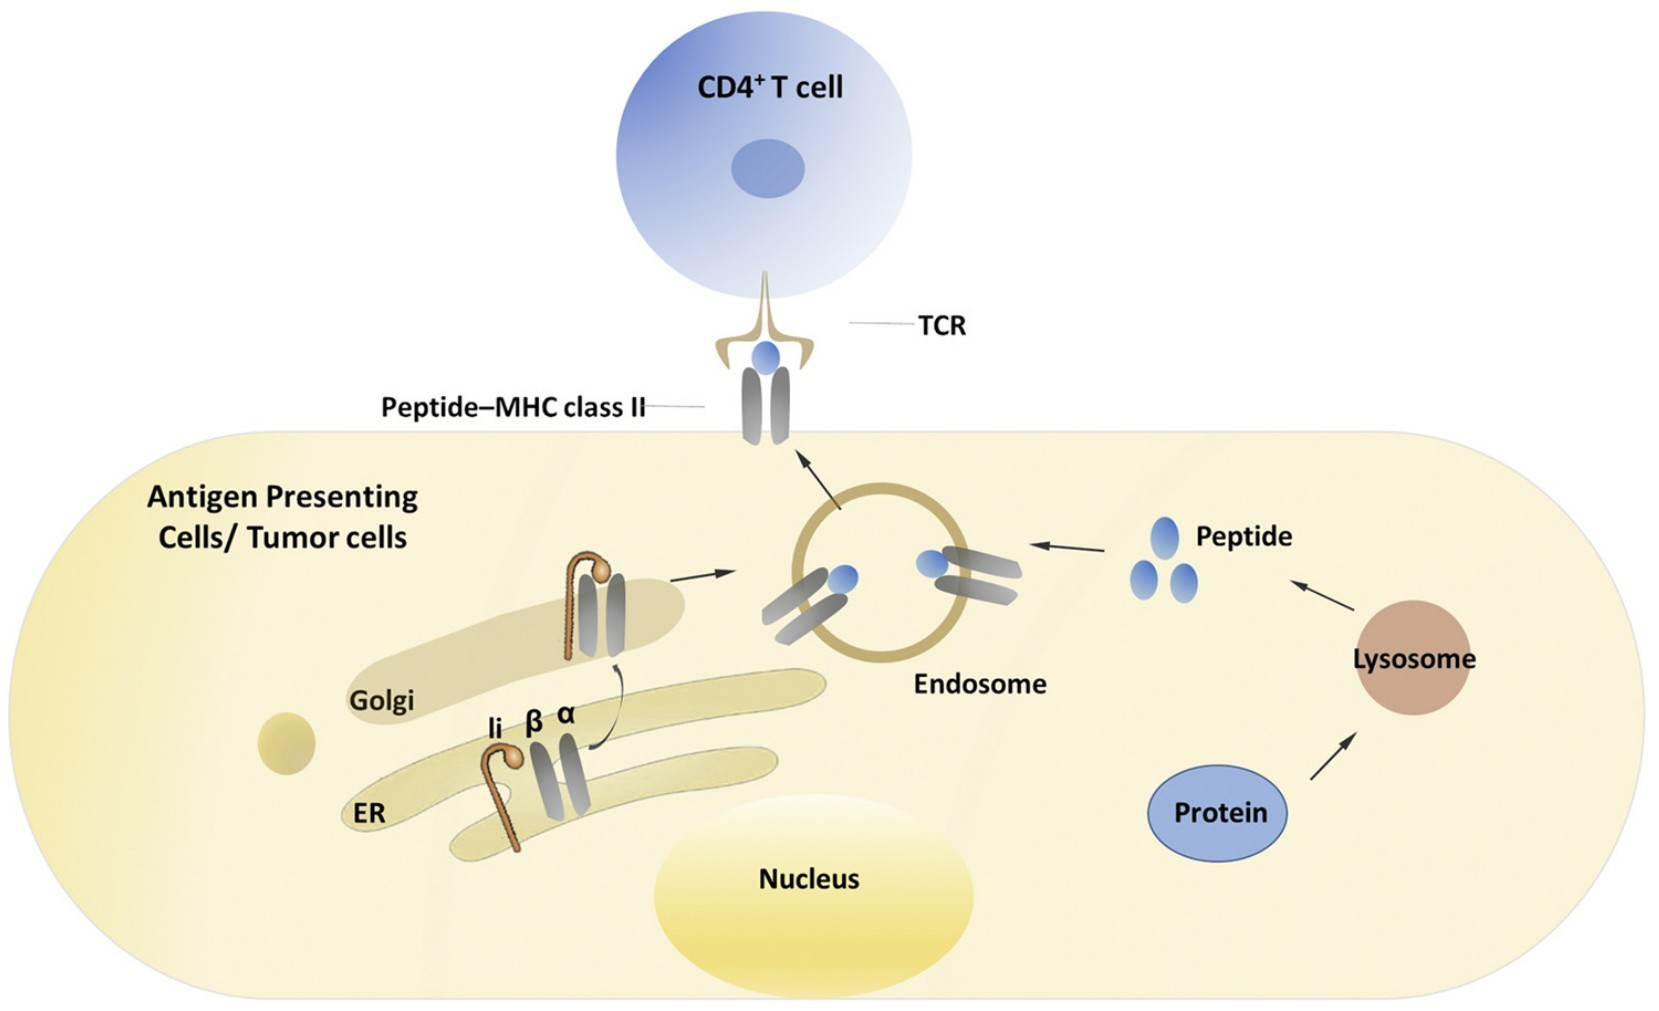
\includegraphics[width=0.8\textwidth]{img/neoantigen/mhc2.jpg}
	\caption{Presentación de antígenos por MHC-II. Fuente: \cite{zhang2019application}}
	\label{fig:mhc2}
\end{figure}

\subsection{Neo antígenos}

Es una proteína que se forma en las células de Cáncer cuando ocurre mutaciones en el DNA. Los neo antígenos cumplen un rol importante al estimular una respuesta inmune en contra de células de Cáncer. En la actualiadad, se estudia su uso en el desarrollo de vacunas contra el Cáncer \cite{NCIdictionary2022}. Una característica importante de los neo antígenos, es que solo están presentes en células tumorales y no en células sanas, debido a eso son considerados factores clave en la inmunoterapia del Cáncer \cite{borden2022cancer}. En la actualidad hay varios métodos para detectar a predecir neo antígenos, pero solo una pequeña porción de ellos logran estimular al sistema inmune \cite{chen2021challenges, hao2021improvement}.

 Este proceso para la detección de neo antígenos, generalmente consiste en: (1) extracción del tejido tumoral, (2) identificación de mutaciones, (3) detección de neo antígenos y predicción de inmunogenicidad, (4) desarrollo de experimentos in vitro y (5) desarrollo de la vacuna \citep{de2020neoantigen, peng2019neoantigen} (ver Figura \ref{fig:process}). \\

\begin{figure}[H]
	\centering
	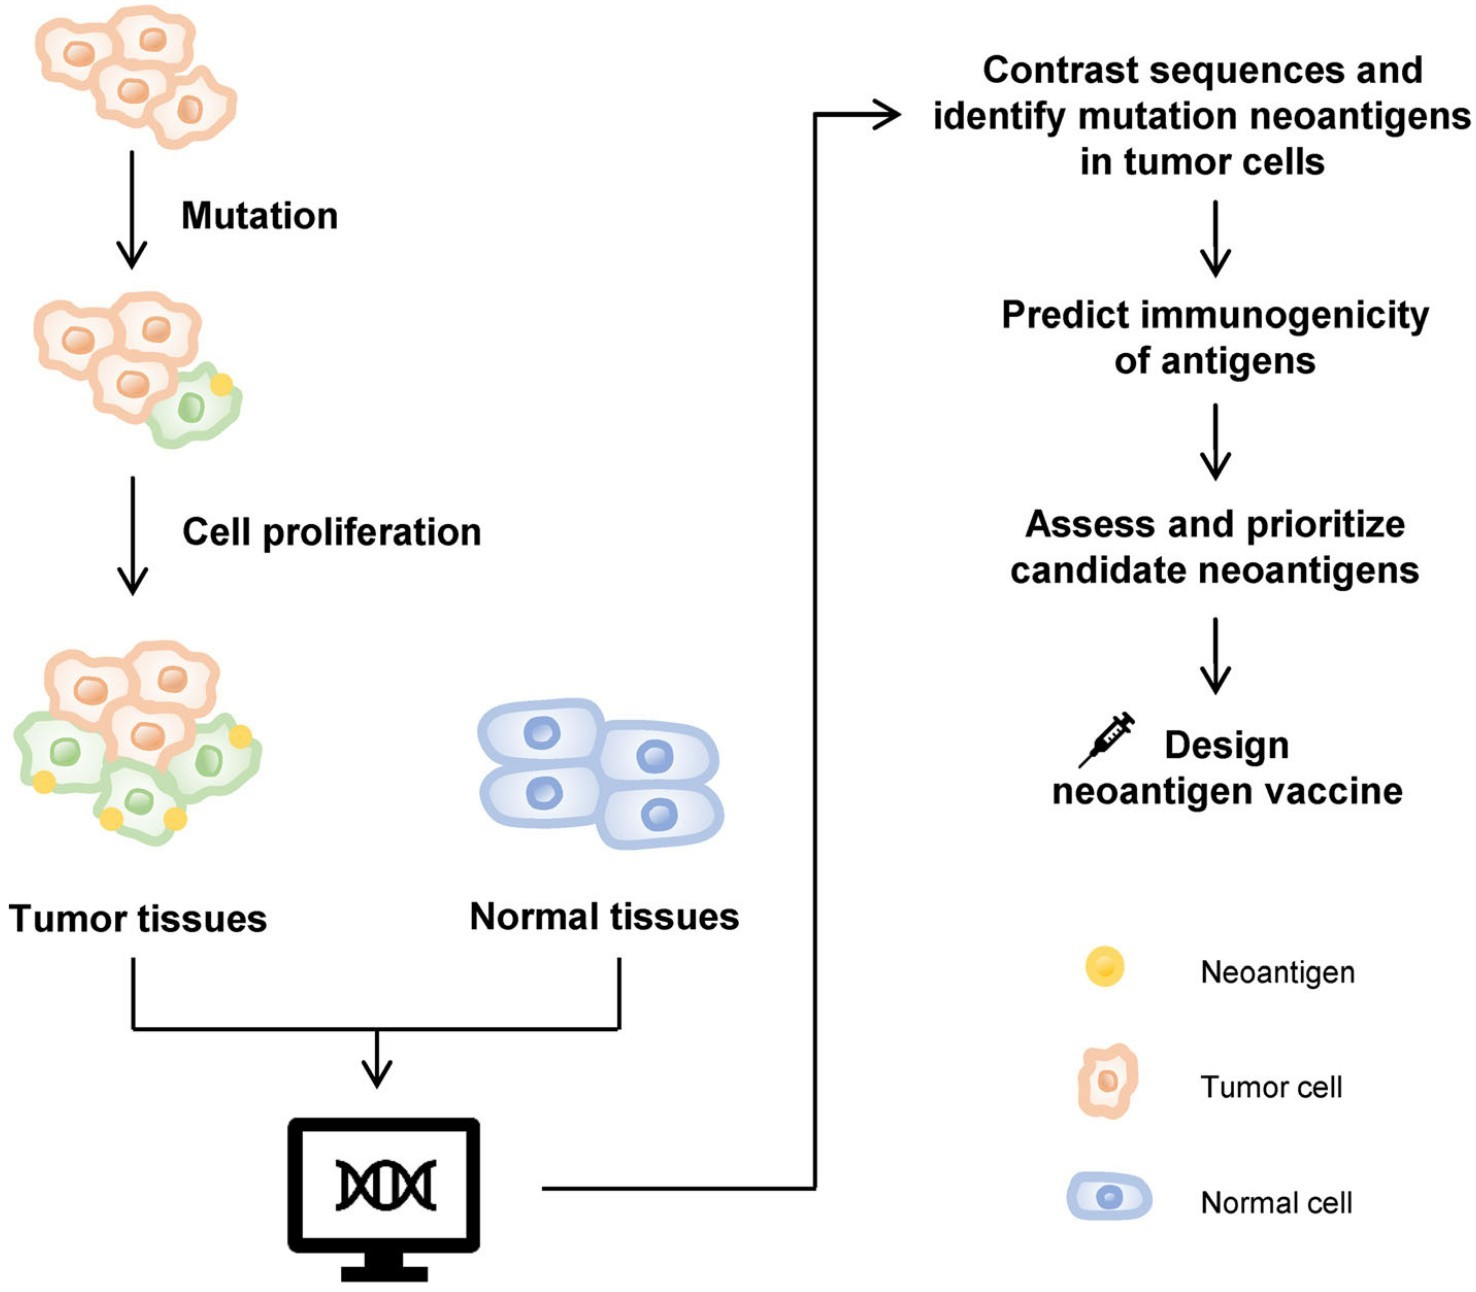
\includegraphics[width=0.7\textwidth]{img/neoantigen/process}	
	\caption{Proceso para la detección de neo antígenos y generación de vacunas personalizadas. Fuente: \citep{de2020neoantigen} }
	\label{fig:process}
\end{figure}


\section{\textit{Machine Learning}}

\textit{Machine Learning} (ML) es una categoría de algoritmos computacionales capaces de emular algunas acciones inteligentes. Es el resultado de varias disciplinas como: inteligencia artificial, probabilidad, estadística, ciencia de la computación, teoría de la computación, psicología y filosofía \citep{el2022machine}. \textit{Machine Learning}  tiene varias definiciones, pero una de las mas acertadas, según \cite{samuel1967some}: ``Campo de estudio que brinda a las computadoras la habilidad de aprender sin haber sido explicitamente programado''. \\





\subsection{Algoritmos de aprendizaje}

Un algoritmo de aprendizaje o \textit{machine learning algorithm}, es aquel algoritmo que no debe ser programado explícitamente, este aprende de la experiencia, a partir de datos \citep{Goodfellow2016}.  Según \cite{mitchell1997machine}: ``A computer program is said to learn from experience \textit{E} with respect to some class of tasks \textit{T} and performance measure \textit{P}, if its performance at tasks in \textit{T}, as measured by \textit{P}, improves with experience \textit{E}''. La traducción a español indicaría: ``Un programa de computadora puede aprender de una experiencia \textit{E}, para una tarea \textit{T} y con una métrica de desempeño \textit{P}, si el desempeño de la tarea \textit{T}, medido con \textit{P}, mejorar con la experiencia \textit{E}''. Esto, nos da a entender que un programa de computadora puede aprender si mejora su desempeño según aumente su experiencia o datos.



\subsubsection{La tarea, \textit{T}}

La tarea \textit{T} de ML, puede ser descrito como de la forma en que el sistema de ML procesa una muestra o ejemplo. Según \cite{Goodfellow2016} las tareas más comunes de ML son:

\begin{itemize}
	\item \textbf{Clasificación}. En este caso, el algoritmo de ML debe predecir la clase a la que pertenece la muestra. Entonces, al algoritmo debe producir una función: $f: \mathbb{R}^n \rightarrow \{ 1, ..., k \}$. También puede escribirse como: $y = f(x)$, aquí $x$ representa la entrada y la función $f$ determinará la clase a la que pertenece.
	
	\item \textbf{Regresión}.  El algoritmo debe producir una función: $f: \mathbb{R}^n \rightarrow \mathbb{R}$. Es decir, dada como entrada un vector $x$ de reales, el algoritmo de ML debe predecir un valor en los números reales.
	
	\item \textbf{Transcripción}. En este caso, dada como entrada datos no estructurados, el algoritmo de ML debe generar información de forma textual. Por ejemplo: dada una imagen como entrada, la salida sería el texto encontrado en la imagen.
	
	\item \textbf{Maquinas de traducción}. Como el nombre indica, la entrada es un texto en un lenguaje y la salida es un texto en otro lenguaje.
	
	\item \textbf{Salida estructurada}. En este caso la salida es un vector o alguna estructura de datos de varios valores. El procesamiento natural de lenguaje es un buen ejemplo, la entrada es un texto y la salida es un árbol que denota la estructura gramatical y semántica de la entrada.
	
	\item \textbf{Detección de anomalías}. En este tipo de problemas el algoritmo de ML, busca detectar eventos anómalos, es decir muestras que no corresponden a la distribución normal de los datos. Un ejemplo, es la detección de transacciones fraudulentas.
	
	\item \textbf{Síntesis y muestreo}. En este caso, el algoritmo de ML debe generar nuevas muestras a partir de un conjunto de entrenamiento. Esto se aplica en los videojuegos, para la generación automática de texturas para objetos de gran tamaño.
	
	
	

\end{itemize}

\subsubsection{El desempeño, \textit{P}}


Es muy importante medir el desempeño de un algoritmo de ML, usualmente la métrica utilizada puede variar según la tarea \textit{T}. Para tareas de clasificación, usualmente se suele aplicar \textit{Precision} y \textit{Recall}, estos estan detallados en las Ecuaciones \ref{eq:presicion} y \ref{eq:recall} respectivamente \citep{dalianis2018evaluation}.


\begin{equation} \label{eq:presicion}
	Precision: P = \frac{tp}{tp + fp}
\end{equation}

\begin{equation} \label{eq:recall}
	Recall: R = \frac{tp}{tp + fn}
\end{equation}

\textit{tp}, hace referencia a la cantidad de muestras que eran verdaderas y han sido reconocidas como verdaderas; \textit{fp}, son las muestras que eran falsas, pero fueron reconocidas como verdaderas; \textit{fn}, son las muestras que eran negativas y fueron reconocidas como negativas. Otra métrica importante es el \textit{F-score}, este puede ser definido como el peso promedio de \textit{Precision} y \textit{Recall}  \citep{dalianis2018evaluation}. En la Ecuación \ref{eq:fbeta}, presentamos la definición.


 
\begin{equation} \label{eq:fbeta}
	F-score: F_\beta = (1 + \beta^2) * \frac{P*R}{\beta^2*P + R}
\end{equation}

Cuando $\beta = 1$:
 
\begin{equation} \label{eq:f1}
	F-score: F_1 = 2 * \frac{P*R}{P + R}
\end{equation}

Finalmente otra métrica, aunque no muy recomendada para datos no balanceados es el \textit{accuracy}. Este representa el porcentaje de muestras reconocidas correctamente.

\begin{equation} \label{eq:f1}
	Accuracy: acc = \frac{tp + tn}{ tp +tn +fp +fn}
\end{equation}


Para otro tipo de problemas, como regresión se puede aplicar el \textit{error rate}, esta es una medida en los números reales y nos indica que tan diferente es la predicción realizada por un algoritmo de ML \cite{Goodfellow2016}.


\subsubsection{La experiencia, \textit{E}}

Según el tipo de experiencia que realizan los algoritmos de ML, se pueden clasificar en: Aprendizaje supervisado y Aprendizaje no supervisado \cite{Goodfellow2016}.

\begin{itemize}
	\item \textbf{Aprendizaje supervisado}. En este caso, cada muestra par el entrenamiento tiene los datos de entrada $x$ y una etiqueta $l$. La idea es que el algoritmo de ML, pueda aprender de estos datos y luego realizar predicción de la etiqueta $j$ tomando como entrada sólo los datos $x$.
	
	\item \textbf{Aprendizaje no supervisado}. En este caso, solo se cuenta con muestras no etiquetadas. Entonces el algoritmo   de ML, debe agrupar los datos en \textit{clusters}. Un ejemplo de estos problemas es la segmentación de clientes, segmentación de noticias, etc.
\end{itemize}



% queda pendiente hablar sobre regresión lineal, logistica y redes neuronales


\subsection{Redes neuronales}

Uno  de los modelos mas representativos de ML son la redes neuronales. Estas se basan en unidades llamadas neuronas (perceptron). En la Figura \ref{fig:neuron}, se muestra esta representación, donde $x_i$, representa un atributo, $w_i$ es el peso que se asigna al atributo $x_i$, de esta forma la neurona representa el resultado de multiplicar un peso a un atributo: $\sum_{i=1}^{d} x_i \cdot w_i$, una representación vectorial sería: $\textbf{x}^T\textbf{w}$ \citep{nielsen2015neural}. Luego, a dicho resultado se aplica una función de activación, la función mas utilizada es la función sigmoidea (Equación \ref{eq:sigmoidea} y \ref{eq:sigmoidea2}).  

\begin{equation}\label{eq:sigmoidea}
	\sigma (z) = \frac{1}{1 + e^{-z}}
\end{equation}

, donde $z = \sum_{i}^{} w_i \cdot x_i - b$.

\begin{equation}\label{eq:sigmoidea2}
	\frac{1}{1 + e^{-\sum_{i}^{} w_i \cdot x_i - b}}
\end{equation}

%Pero, existen otras funciones de activación que se pueden aplicar según el problema: Softmax: $\phi(x) = \frac{e^{x_i}}{\sum_{j=0...k^{e^{x_j}}} }; i = 0, 1, 2, ..., k$, función tangente hiperbolica: $\phi(x) = \frac{e^x - e^{-x}}{e^x + e^{-x}}$ y RELU: $\phi(x) = max(0, x)$.

\begin{figure}[H]
	\centering
	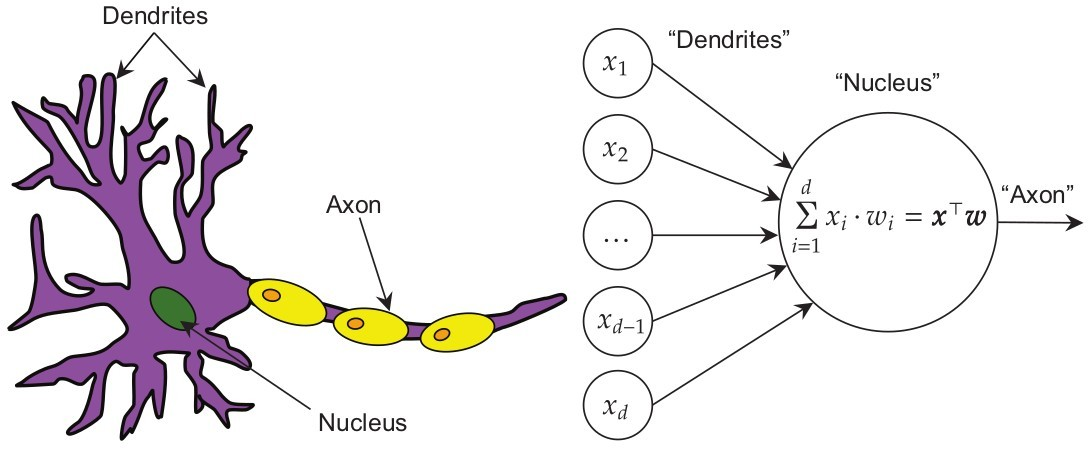
\includegraphics[width=0.8\textwidth]{img/neoantigen/neuron}
	\caption{Representación de una neurona. Fuente: \cite{insideDL2022}.}
	\label{fig:neuron}
\end{figure}

El perceptron, es capaz de solucionar varios problemas, pero para casos complejos puede formar una red, como se presenta en la Figura \ref{fig:nn}.

\begin{figure}[H]
	\centering
	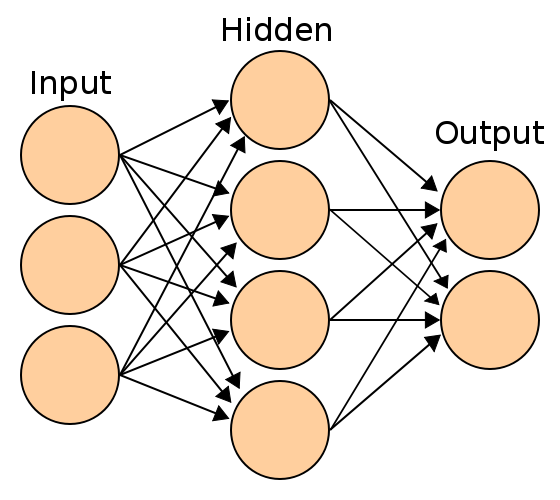
\includegraphics[width=0.35\textwidth]{img/neoantigen/nn2}
	\caption{Representación de una red neuronal. }
	\label{fig:nn}
\end{figure}

\section{\textit{Deep learning}}

\textit{Deep learning} (DL) es una subcategoría de \textit{Machine Learning}, a diferencia de los algoritmos tradicionales de ML, usualmente DL trata con señales sin pre-procesamiento, los modelos (basados en redes neuronales) son mucho mas complejos tanto en dimensión como en el método de aprendizaje \citep{el2022machine}. Por ejemplo, en la Figura \ref{fig:dl}, presentamos la relación entre inteligencia arficial, ML y DL, de ahí podemos concluir que ML es parte de la IA y DL es parte de ML \citep{el2022machine}.

\begin{figure}[H]
	\centering
	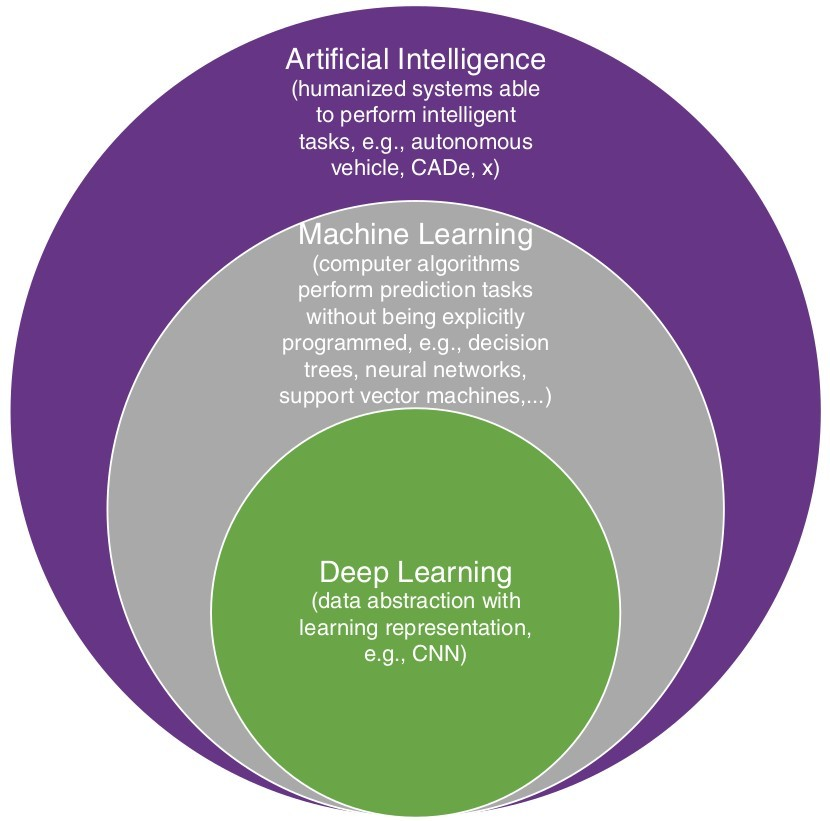
\includegraphics[width=0.5\textwidth]{img/neoantigen/dl}
	\caption{Relación entre Inteligencia Artificial, \textit{Machine Learning} y \textit{Deep Learning}. Fuente: \cite{el2022machine}.}
	\label{fig:dl}
\end{figure}


\subsection{\textit{Deep Feedforward networks}}

\textit{Deep Feedforward networks} son perceptrones multicapa o \textit{multilayer perceptrons}(MLP). Su objetivo es aproximar una función $f^*$, para el caso de clasificación, podría modelarse como $ y=f^*(x)$. Luego, un \textit{feedforward network}, define un mapeo $y = f(x;\theta)$ y aprende los valores de los parametros $\theta$ \cite{Goodfellow2016}. Entonces un \textit{Deep Feedforward networks}, es una red neuronal tradiconal pero con un número grande de neuronas y capas (Figura \ref{fig:dnn}). Existen muchos tipos de \textit{Deep Feedforward networks}, estas serán detalladas en los siguientes apartados.

\begin{figure}[H]
	\centering
	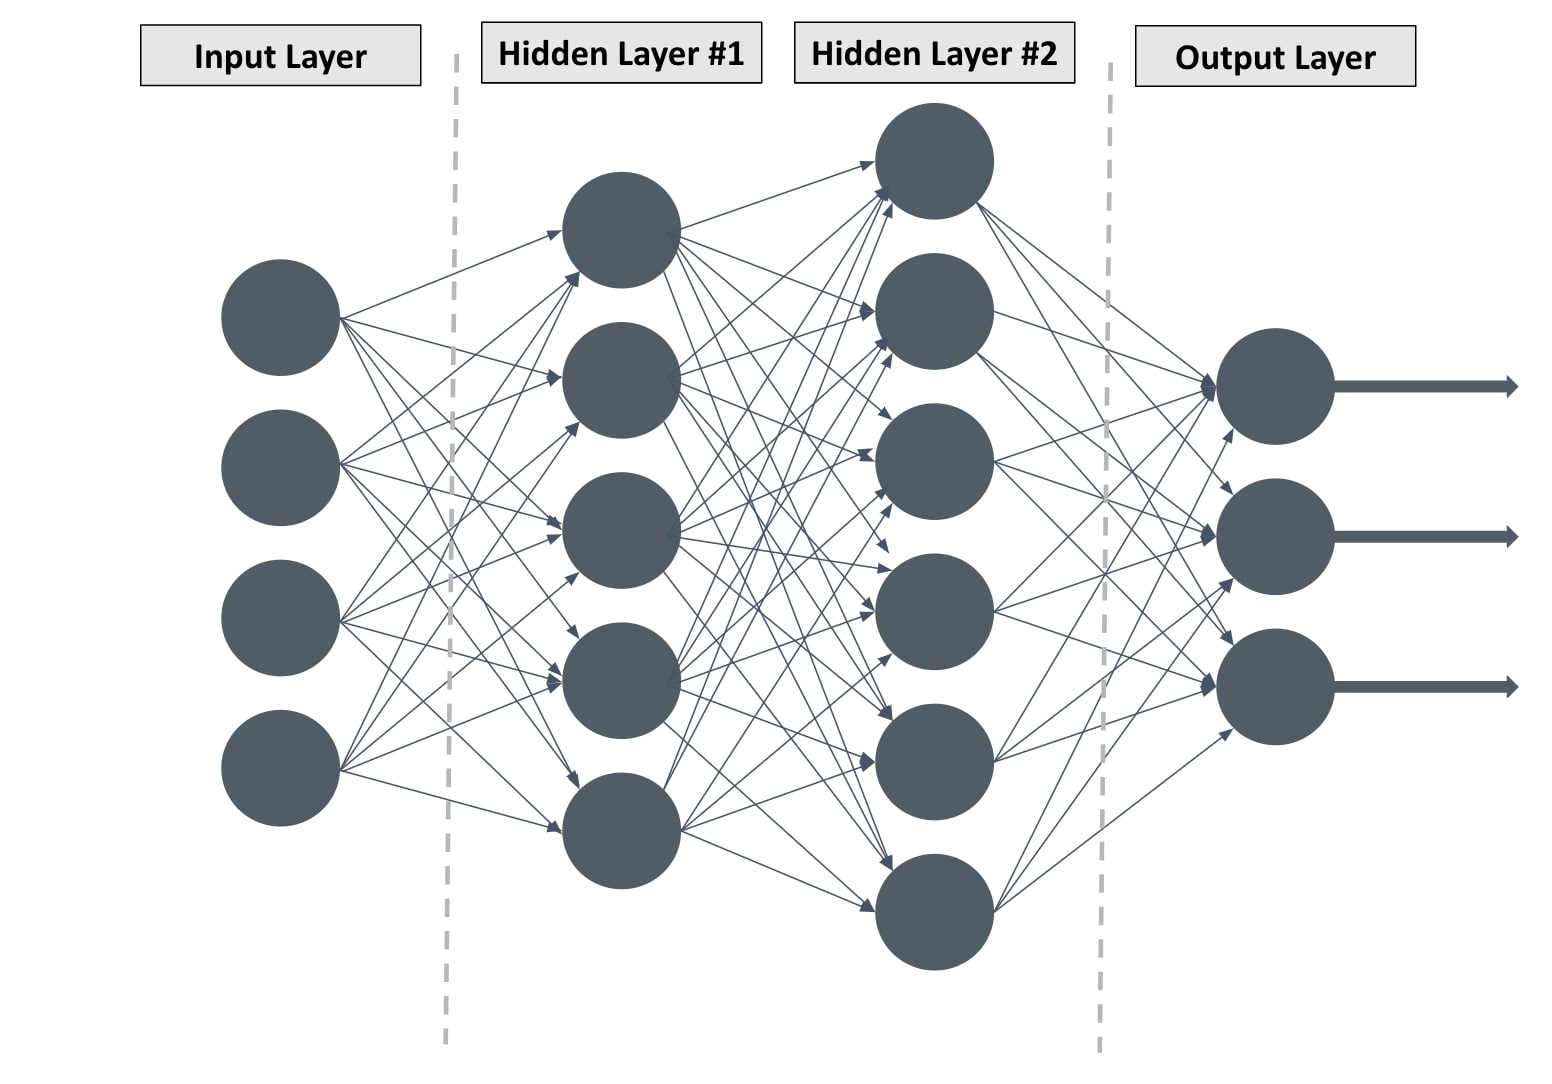
\includegraphics[width=0.7\textwidth]{img/neoantigen/deep_nn}
	\caption{Representación de un \textit{Deep Feedforward Network}. Fuente: \cite{el2022machine}.}
	\label{fig:dnn}
\end{figure}


\subsection{\textit{Convolutional Neural Networks}}

Una \textit{Convolutional Neural Networks} (CNN), es una red neuronal basada en la operación de convoluciones (utilizada en procesamiento de imágenes). Generalmente estas redes neuronales se aplican a problemas de visión computacional \citep{zhang2021dive}. La operación básica es la convolución, esta se presenta en la Figura \ref{fig:cnn}. Se toman pequeñas ventanas de una imagen y se realiza el producto punto con un \textit{kernel} ya establecido. Según los diferentes valores del \textit{kernel}, se pueden obtener diferentes resultados en la imagen de salida como: detección de bordes, suavizados, dilatación, etc.


\begin{figure}[H]
	\centering
	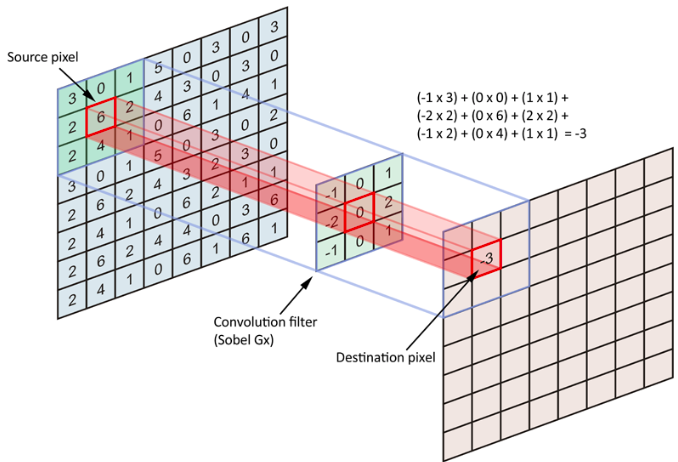
\includegraphics[width=0.7\textwidth]{img/neoantigen/cnn}
	\caption{Ejemplo de una convolución en procesamiento de imágenes. Fuente: \cite{Shuchen2022}.}
	\label{fig:cnn}
\end{figure}

Con inspiración en la operación de convolución, se plantean las CNN por primera vez por \cite{lecun1998gradient}. En la Figura \ref{fig:cnn3}, se presenta la LeNet-5, planteado por los autores. Luego, surgen diversa propuestas como AlexNet \citep{krizhevsky2012imagenet}, VGGNet \citep{simonyan2014very}, GoogleNet \citep{szegedy2015going} y ResNet \citep{he2016deep}.

\begin{figure}[H]
	\centering
	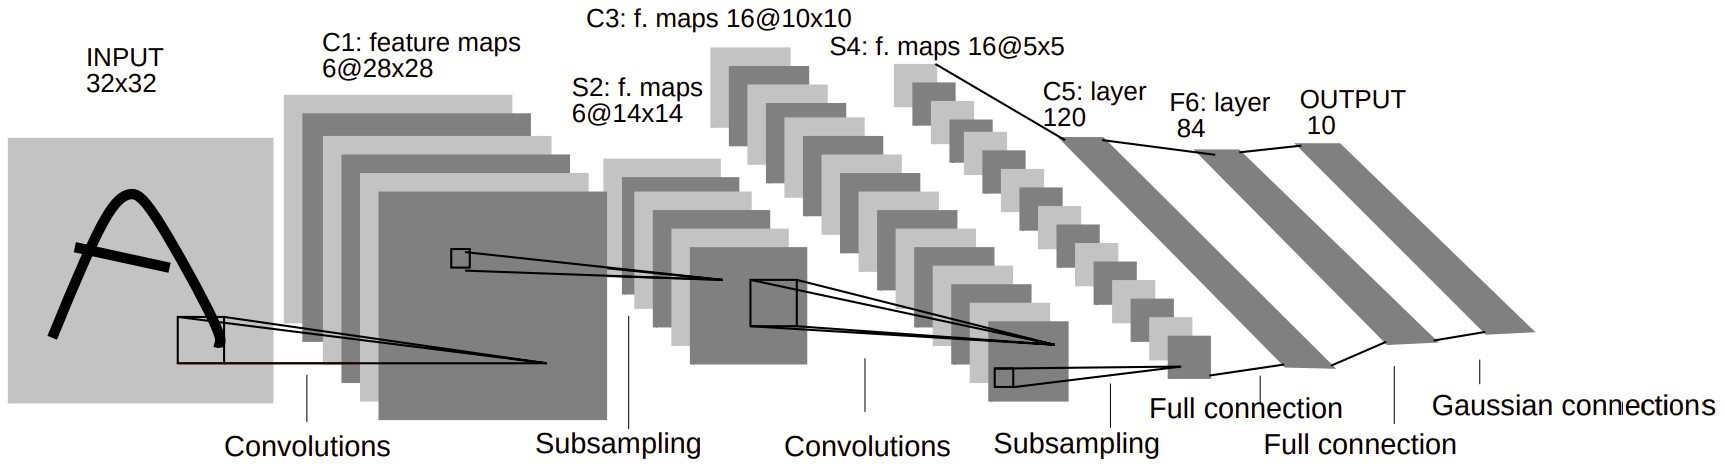
\includegraphics[width=\textwidth]{img/neoantigen/cnn3}
	\caption{Arquitectura de LeNet-5, una CNN para el reconocimiento de digitos. Fuente: \cite{lecun1998gradient}.}
	\label{fig:cnn3}
\end{figure}


\subsection{\textit{Recurrent Neural Networks}}

Mientras que las CNN están especializadas para manejar información espacial, las \textit{Recurrent Neural Networks} (RNN), se especializan en información secuencial  \citep{zhang2021dive}. En este campo, se habla del tiempo como una variable y se tratan problemas de series temporales por ejemplo.

El término RNN, aparece por primera vez en los trabajos de \cite{rumelhart1985learning} y \cite{jordan1997serial}. Algunos autores, comentan también que el inicio de las RNN fue con las redes de Hopfield  \citep{hopfield1982neural}. En general estas RNN, tienen dos entradas: estado actual y estado anterior; luego la RNN predice el siguiente estado. El problema de estas redes neuronales surgen por una falta de memoria, es decir cuando tenemos varios estados, el estado inicial va a influenciar cada vez menos a los estados futuros.

Como alternativa de solución al problema mencionado anteriormente, surgen Long Short-Term Memory, propuesta por \cite{hochreiter1997long}. Una red neuronal LSTM, es capaz de recordar un dato relevante de una secuencia y almacenarlo varios instantes de tiempo. En la Figura \ref{fig:lstm}, explicamos brevemente el funcionamiento de LSTM, los datos que ingresan a una compuerta (\textit{gate}), son los datos de entrada en un tiempo específico y el estado oculto anterior. Luego, es procesado por tres capas totalmente conectadas: \textit{input gate}, \textit{forget gate} y \textit{output gate} \citep{zhang2021dive}.

\begin{figure}[H]
	\centering
	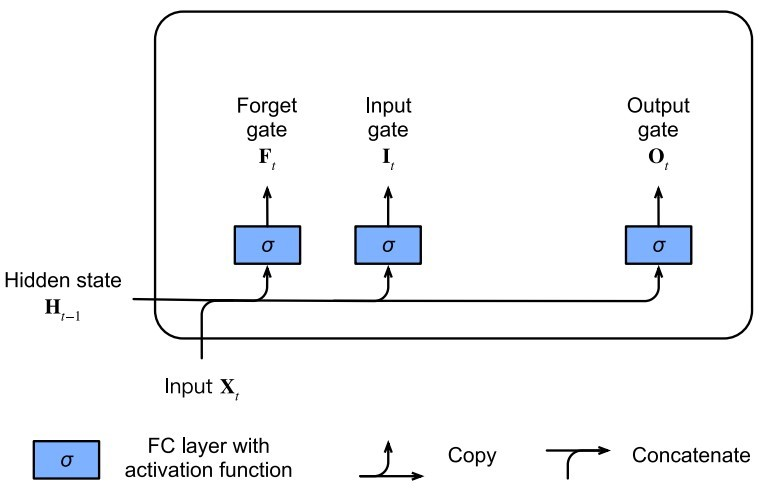
\includegraphics[width=0.7\textwidth]{img/neoantigen/lstm}
	\caption{Ejemplo del procesamiento del \textit{input gate}, \textit{forget gate} y \textit{output gate} de LSTM. Fuente: \cite{zhang2021dive}.}
	\label{fig:lstm}
\end{figure}

\subsection{\textit{Transformers}}

Los \textit{Transformers} son propuestas por \cite{vaswani2017attention}, para dar solución al problema de \textit{long-range dependency}. Por ejemplo el autor comenta: ``The Transformer is the first transduction model relying entirely on self-attention to compute representations of its input and output without using sequence-aligned RNNs or convolution''. Del enunciado anterior, \textit{transduction} hace referencia a la conversión secuencias de entrada hacia otro formato. Otro termino interesante es \textit{self-attention} (Figura \ref{fig:transformer}), este permite al modelo mirar hacia otras palabras en la secuencia de entrada para tener un mejor entendimiento de cierta palabra en la secuencia  \citep{Kelvin_transformer2022}.  

\begin{figure}[H]
	\centering
	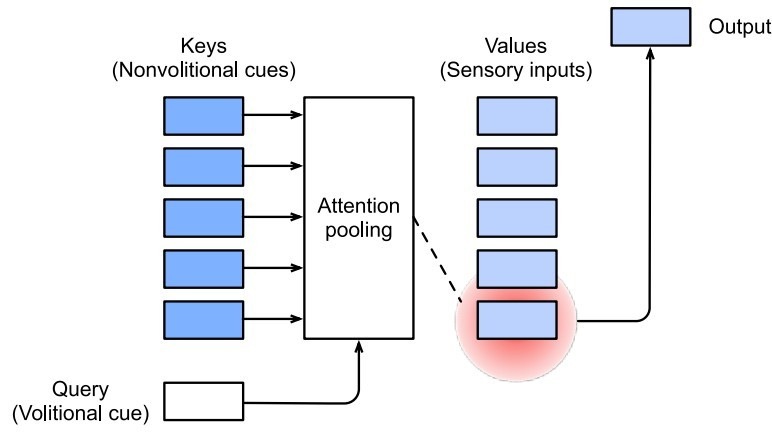
\includegraphics[width=0.7\textwidth]{img/neoantigen/transformer}
	\caption{ejemplo del mecanismo de atención de una red \textit{Transformer}. Fuente: \cite{zhang2021dive}.}
	\label{fig:transformer}
\end{figure}


\subsection{\textit{BERT}}

\textit{Bidirectional Encoder Representations from Transformers (BERT)}, propuesta por \cite{devlin2018bert}, está inspirada por la red \textit{Tranformer} y su mecanismo de atención, la cuál entiende la relación contextual entre diferentes palabras. A diferencia de una RNN, BERT no tiene dirección, es decir lee la secuencia entera. Esta característica, le permite al modelo aprender información contextual de una palabra con respecto a las otras \citep{Kelvin_transformer2022}.








%EOF
 % Introduction
%% ------------------------------------------------------------------- %%
\chapter{Estado del Arte}
\label{cap:estadodelarte}
\lhead{\emph{Estado del Arte}} 

En este capítulo detallamos la metodología utilizada para realizar una Revisión Sistemática de la Literatura (RSL) referente a los métodos basados en Transformer y redes neuronales que utilicen mecanismos de atención para la detección de neoantígenos.

\section{Revisión Sistemática de la Literatura (RSL)}

Nuestro enfoque principal se centra en la priorización de neoantígenos (ver Figura 	\ref{fig:etapas}), ya que esta área ha sido objeto de una cantidad significativa de investigaciones que utilizan Transformers. Además, integramos análisis de pipelines y estudios de ensayos clínicos para obtener información sobre los hallazgos más recientes en cuanto a la aplicación de la detección de neoantígenos en vacunas personalizadas contra el cáncer. 

\begin{figure}[h]
	\centering	
	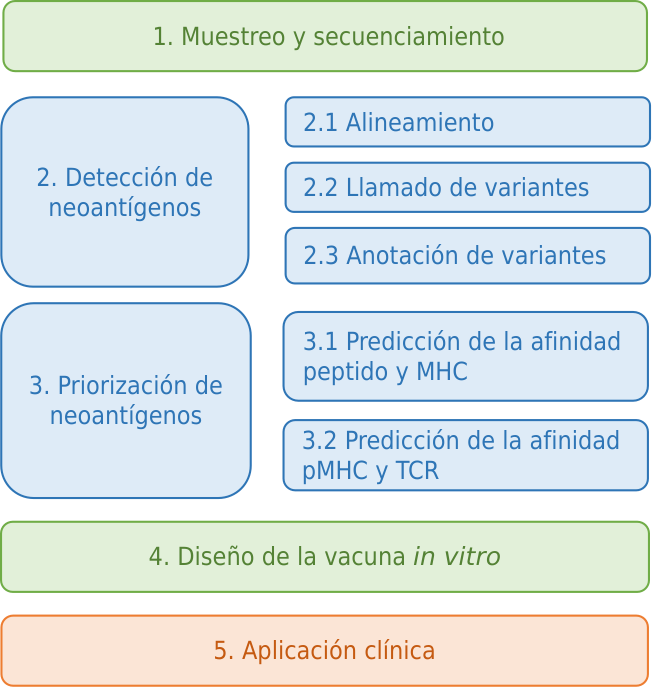
\includegraphics[width=0.5\textwidth]{img/pipeline/pipeline_spanish}	
	\caption{Una visión general de cada fase del proceso de generación de vacunas personalizadas basadas en neoantígenos.}
	\label{fig:etapas}
\end{figure}


Según las cadenas de búsqueda de la Tabla \ref{tab:search} y considerando solo trabajos publicados a partir de 2018, se analizaron los títulos de los artículos, obteniendo un total de 151 artículos. Luego, se seleccionó un subconjunto en función de los criterios de inclusión: artículos con una categoría ERA (A o B) o artículos de revistas en los cuartiles Q1/Q2. Al final de esta etapa, se obtuvieron 79 artículos.


\begin{table}
	\caption{Cadenas de búsqueda utilizadas en la RSL para cada fase de detección de neoantígenos.}
	\label{tab:search}
	\centering
	\setlength{\tabcolsep}{0.5em} % para el espaciado horizontal
	{\renewcommand{\arraystretch}{1.7}% para el espaciado vertical
		\begin{tabular}{p{3cm}p{10cm}}
			\textbf{Categoría} & \textbf{Cadena de búsqueda} \\ \hline
			Priorización de neoantígenos & (mhc OR hla) AND (peptide OR epitope OR antigen) AND (specificity OR immunogenicity OR binding OR affinity OR predict* OR detection OR presentation OR classification) AND (transformer* OR bert* OR attention OR 'transfer learning' OR method* OR predict*)'', ( tcr OR 't cell' OR t-cell) AND (mhc OR peptide OR epitope OR antigen) AND (specificity OR immunogenicity OR binding OR affinity OR predict* OR detection OR presentation OR classification) AND (transformer* OR bert* OR attention OR 'transfer learning' OR method* OR predict*) \\
			
	
			Pipelines & (pipeline OR toolkit) AND ( tcr OR 't cell' OR t-cell OR mhc OR hla OR peptide OR epitope OR antigen* OR neoantigen*) (pipeline OR tool* OR workflow OR application OR web* ) AND ( peptide OR epitope OR antigen* OR neoantigen* OR neoepito*) AND (immunotherapy OR detection OR identify* OR predict* OR presentation*)\\
			
			Ensayos clínicos &  (neoantigen OR neoepitope OR denditric cell) AND (vaccines OR immunology)
			
	\end{tabular}}
\end{table}




\section{Resultados de la RSL}

\subsection{Detección de neoantígenos}

La detección de neoantígenos se basa en la identificación inicial de candidatos, seguida de su posterior priorización. En esta sección, explicaremos el proceso de detección de candidatos a neoantígenos (etapa 2 en la Figura \ref{fig:etapas}).

Durante esta etapa, se utilizan datos de secuenciación de ADN (DNA-seq) y de ARN (RNA-seq) para identificar candidatos a neoantígenos. Sin embargo, en este campo, se han adoptado ampliamente varias herramientas bien establecidas, y los Transformers no se utilizan regularmente. En primer lugar, se encarga de tomar datos de DNA-seq, RNA-seq y \textit{Mass Spectrometry} (MS) como entrada. Luego, procede a alinear estas secuencias utilizando herramientas como BWA-MEM y Bowtie2. Además, STAR podría ser utilizado porque alinea muestras de tumores de manera más efectiva \citep{rubinsteyn2018computational}. La salida de esta etapa consiste en archivos de alineación BAM. Para la llamada de variantes, se podrían emplear MuTect y Strelka. Posteriormente, la información de ambos métodos se podría combinar, siguiendo el enfoque utilizado por \cite{zhou2021prioritizing} y \cite{rubinsteyn2018computational}. La salida consiste en archivos VCF. A continuación, está la etapa de anotación de variantes, donde se utilizan archivos con formato VCF para derivar péptidos generados a partir de estas variaciones o mutaciones; Isovar y ANNOVAR podrían ser utilizados en esta tarea. Finalmente, para determinar el tipo de HLA del paciente, la herramienta OptiType es una opción. Al final, tenemos varios candidatos a neoantígenos y los tipos de HLA del paciente.

\subsection{Priorización de neoantígenos}

La priorización de neoantígenos es la tercera etapa en el desarrollo de vacunas contra el cáncer (Figura \ref{fig:etapas}). En esta etapa, se toman los candidatos a neoantígenos y se predice su afinidad con el MHC, un problema conocido como predicción del enlace pMHC. Luego, este complejo pMHC se utiliza para predecir la interacción con el TCR. Ambos problemas toman dos secuencias de proteínas como entrada, y el objetivo es predecir su afinidad (regresión) o unión (clasificación). 


\subsubsection{Bases de datos}

Para priorizar neoantígenos, los investigadores a menudo recopilan muestras de diversas fuentes, generalmente extrayendo datos de estudios previos y recursos similares. Sin embargo, existen conjuntos de datos públicos disponibles, como se enumeran en la Tabla \ref{tab:bd}, que se centran específicamente en la interacción entre péptidos y MHC (péptido-MHC)  \citep{wu2018tsnadb, zhou2019neopeptide, tan2020dbpepneo, lu2022dbpepneo2}, así como en la interacción entre pMHC y TCR \citep{shugay2018vdjdb, bagaev2020vdjdb}. Es importante destacar que un estudio reciente proporciona estructuras tridimensionales de péptidos y HLA, lo que introduce una nueva perspectiva de investigación. Finalmente, la \textit{Immune Epitope Database} (IEDB) \citep{vita2019immune} se destaca como un recurso ejemplar en este campo.

\begin{table}[h]
	\caption{Bases de datos públicas de unión pMHC e interacción pMHC-TCR}
	\label{tab:bd}
	\setlength{\tabcolsep}{0.5em} % para el espaciado horizontal
	{\renewcommand{\arraystretch}{1.2}% para el espaciado vertical
		
		\begin{tabular}{lp{1cm}p{3.5cm}p{6cm}}
			\textbf{Nombre} & \textbf{Año} & \textbf{Ref.} & \textbf{Descripción} \\ \hline
			VDJdb           & 2018 & \cite{shugay2018vdjdb, bagaev2020vdjdb} & Base de datos de unión del TCR al pMHC, contiene 5491 muestras. \\
			IEDB            & 2018 & \cite{vita2019immune} & Es la base de datos más grande que contiene información de \textit{epitopes} de células T de humanos y otros organismos. \\
			TSNAdb          & 2018 & \cite{wu2018tsnadb} & Involucra 7748 muestras de mutaciones y HLA de 16 tipos de cáncer. \\
			NeoPeptide      & 2019 & \cite{zhou2019neopeptide} & Incorpora muestras de neoantígenos resultantes de mutaciones somáticas y elementos relacionados. También contiene 1818137 \textit{epitopes} de más de 36000 neoantígenos. \\
			
			pHLA3D          & 2019 & \cite{e2019phla3d} & Presenta 106 estructuras 3D de las cadenas $\alpha$, $\beta 2M$ y péptidos de las moléculas HLA-I. \\
			dbPepNeo        & 2020 & \cite{tan2020dbpepneo} & Contiene muestras validadas de la unión del pMHC a partir de MS. Incluye 407794 muestras de baja calidad, 247 de calidad media y 295 de alta calidad. \\
			dbPepNeo2.0     & 2022 & \cite{lu2022dbpepneo2} & Recopila una lista de neoantígenos y moléculas HLA. Presenta 801 HLAs de alta calidad y 842,289 de baja calidad. Además, 55 neoantígenos de clase II y 630 neoantígenos con unión al TCR. \\
			IntroSpect      & 2022 & \cite{zhang2022introspect} & Es una herramienta para construir bases de datos sobre la unión pMHC. Utiliza datos de MS. \\
			IPD-IMGT    & 2022 & \cite{robinson2020ipd} & Tiene 25000 moléculas MHC y 45 \textit{alleles}. \\
		\end{tabular}
	}
\end{table}

\subsubsection{Predicción de la unión pMHC}

Los enfoques para predecir la unión pMHC se pueden clasificar ampliamente en dos categorías: métodos \textit{allele-specific} y métodos \textit{pan-specific}. Los métodos \textit{allele-specific} implican entrenar un modelo distinto para cada \textit{allele} específico, mientras que los métodos \textit{pan-specific} implican el entrenamiento de un modelo universal aplicable a una variedad de \textit{alleles}. Luego, en la Tabla \ref{tab:transformes}, presentamos una comparación de modelos Transformer y métodos de aprendizaje profundo que utilizan mecanismos de atención.

Dado que trabajamos con entradas de proteínas, cada aminoácido se representa utilizando una fila de la matriz BLOSUM. Algunos estudios han utilizado BLOSUM62 \citep{jin2021deep, ye2021mathla, zhao2019peptide, o2018mhcflurry} y BLOSUM50 \citep{yang2021deepnetbim, hu2019acme}. Además, ciertos autores han utilizado una combinación de codificación one-hot y codificación BLOSUM \citep{liu2021deepseqpanii, jokinen2021predicting, zeng2019quantification, zeng2019deepligand}. Alternativamente, se han empleado métodos como el codificador universal de Google \citep{kubick2021predicting}, AAindex \citep{kawashima2000aaindex, li2021deepimmuno} (una base de datos de índices numéricos que representan propiedades fisicoquímicas y bioquímicas de los aminoácidos), coordenadas tridimensionales de aminoácidos \citep{shi2020deepantigen}, y la consideración de las propiedades fisicoquímicas de aminoácidos individuales \citep{moris2021current, montemurro2021nettcr, luu2021predicting}. Más recientemente, algunos estudios han incorporado ligandos eluídos de la membrana celular, extraídos mediante datos MS \citep{zhouprioritizing, reynisson2020netmhcpan, reynisson2020improved, o2020mhcflurry, alvarez2019nnalign_ma}.

Actualmente, NetMHCPan4.1 \citep{reynisson2020netmhcpan} es un método de referencia, este es una red neuronal artificial profunda  que consiste en 40 redes neuronales artificiales ensambladas; cabe destacar que maneja eficazmente conjuntos de datos de MS, al igual que el MHCflurry2.0 \citep{o2020mhcflurry}.

\begin{table}[h]
	\caption{Transformers y métodos de aprendizaje profundo con mecanismos de atención utilizados para la predicción de la unión pMHC.}
	\label{tab:transformes}
	\setlength{\tabcolsep}{0.5em} % para el espaciado horizontal
	{\renewcommand{\arraystretch}{1.1}% para el espaciado vertical
		
		\begin{scriptsize}
			
		
		\begin{tabular}{p{2.5cm}p{2.5cm}p{2cm}p{5.5cm}}
			\multicolumn{1}{l}{\textbf{Ref.}}                                   & \textbf{Nombre}             & \textbf{Entrada}            & \textbf{Modelo}     \\  \hline
			
			\cite{hashemi2023improved}&	ESM-GAT  &	One-hot & BERT con transferencia de aprendizaje de ESM1b y ESM2 \textit{fine-tuned} con una \textit{Graph Attention Network} (GAT) al final. Superó a NetMHCpan4.1.	\\
			
			
			\cite{kalemati2023capsnet}&	CapsNet-MHC&	BLOSUM62 & \textit{Capsule Neural Network}, superó a las herramientas de vanguardia para péptidos pequeños de 8 a 11 mer.	\\
			
			\cite{ye2023stmhcpan}&	STMHCpan  &	One-hot & Un modelo Star-Transformer, útil para péptidos de cualquier longitud y ampliable para predecir respuestas de células T.	\\
			
			\cite{jing2023dapnet}&	DapNet-HLA&	\textit{Fused word embedding} & Combina las ventajas de CNN, SENet (para agrupación) y LSTM con atención.	\\
			
			\cite{zhang2022hlab}&	HLAB&	One-hot & BERT del modelo pre-entrenado ProtBert seguido de una BiLSTM.	\\
			
			\cite{wang2022mhcroberta}          & MHC RoBERTa            & One-hot & RoBERTa pre-entrenado seguido de 12 \textit{multi-head self-attention} y capas totalmente conectadas, superó a NetMHCPan3.0.                                                                                          \\
			\cite{chu2022transformer}          & TransPHLA             & One-hot         & Utiliza un mecanismo de self-attention basado en cuatro bloques, superó ligeramente a NetMHCpan4.1 y es más rápido en hacer predicciones.\\
			
			\cite{chen2021jointly}  & CapTransformer            & One-hot   &  Transformer con \textit{cross self-attention} para capturar información local y global.  \\
			
			\cite{gasser2021interpreting}  & ImmunoBERT            & One-hot                     & BERT de TAPE pre-entrenado seguido de una capa lineal. Los autores afirman que los terminales N y C son altamente relevantes después de un análisis con SHAP y LIME.   \\
			
			\cite{cheng2021bertmhc}             & BERTMHC              & One-hot                    & BERT de TAPE pre-entrenado seguido de una capa lineal. Superó a NetMHCIIpan3.2 y PUFFIN.   \\
			
			% CNN y RNN con atención
			\cite{ye2021mathla}         & MATHLA             & BLOSUM                      & 
			Integra BiLSTM con \textit{multi-head self-attention}. Obtuvo una puntuación AUC de 0.964, en comparación con 0.945, 0.925 y 0.905 para NetMHCpan 4.0, MHCflurry y ACME respectivamente  \\
			
			\cite{liu2021deepseqpanii}                    & DeepSeqPanII                            & BLOSUM62 y one-hot& Tiene dos capas LSTM, un bloque de atención y tres capas totalmente conectadas. Obtuvo mejores resultados que NetMHCIIpan 3.2 en 26 de 54 alelos.       \\
			
			\cite{yang2021deepnetbim}  & DeepNetBim               & BLOSUM50            & Utiliza CNN separadas para la predicción de la unión pMHC y \textit{immunogenetic} con un módulo de atención. Obtuvo 0.015 MAE para la unión y 94.7 de precisión para la inmunogenicidad.      \\
			
			\cite{jin2021deep}         & DeepAttention Pan        & BLOSUM62            & CNN con un mecanismo de atención. Es \textit{allele-specific} y obtuvo resultados ligeramente mejores que ACME a nivel de \textit{alleles}.     \\
			
			\cite{chen2021ranking}  & SpConvM            &  One-hot, BLOSUM y Deep                     &  Capa 1D de CNN, una capa de atención y una capa totalmente conectada. Además, emplearon \textit{global kernels} para mejorar sus resultados, junto con una combinación de onehot, BLOSUM y Deep.  \\
			
			\cite{venkatesh2020mhcattnnet}         & MHCAttNet        & One-hot            & CNN seguido de una capa de atención para generar un mapa de calor sobre los aminoácidos.     \\
			
			\cite{hu2019acme}          & ACME                     & BLOSUM50     & CNN con atención, extrae patrones interpretables sobre la unión pMHC. Además, obtuvo un SRCC de 0.569, un AUC de 0.9 para HLA-A y 0.88 para HLA-B.  \\    
			
			
			\cite{wu2019deephlapan}                      & DeepHLApan                              & One-hot             & Modelo \textit{allele-specific} con tres capas de GRU Bidireccional (BiGRU) con una capa de atención. Obtuvo una precisión $> 0.9$ en 43 \textit{alleles} HLA.                                               
		\end{tabular}
	\end{scriptsize}
	}
\end{table}

%CNN
Existen modelos de \textit{Convolutional Neural Networks} (CNN) que incorporan un mecanismo de atención, como ACME \citep{hu2019acme}. ACME utiliza una CNN con un módulo de atención que asigna pesos a posiciones de residuos individuales, con el objetivo de asignar mayores pesos a los residuos de mayor importancia en las interacciones pMHC. ACME logró un Coeficiente de Correlación de Rango de Spearman (SRCC) de 0.569, lo cual es superior a NetMHCpan 4.0. A continuación, tenemos MHCAttNet \citep{venkatesh2020mhcattnnet}, que utiliza una CNN seguida de una capa de atención. La capa de atención se utiliza para generar un mapa de calor sobre los aminoácidos, indicando las subsecuencias importantes presentes en la secuencia de aminoácidos. Otro modelo basado en CNN es DeepAttentionPan \citep{jin2021deep}, que utiliza una CNN profunda para codificar péptidos y MHC en vectores de dimensiones $40\times 10 \times 11$ antes de emplear un módulo de atención para calcular pesos posicionales. También contamos con DeepNetBim \citep{yang2021deepnetbim}, que incorpora un módulo de atención similar a ACME y DeepAttentionPan. Sin embargo, utiliza dos CNN separadas para predecir la unión pMHC y la inmunogenicidad, que luego se combinan en las capas finales. Además, en su estudio sobre SpConvM \citep{chen2021ranking}, los autores demostraron que la incorporación de núcleos globales en CNN con atención produjo un mejor rendimiento. Además, sus experimentos incluyeron una comparación de diferentes métodos de codificación de aminoácidos, incluyendo onehot, BLOSUM y Deep. Según sus hallazgos, la combinación de onehot, BLOSUM y Deep juntos dio como resultado mejores resultados. Recientemente, ha surgido el uso de \textit{Capsule Neural Network} (CapsNet) para modelar relaciones jerárquicas. CapsNet-MHC \citep{kalemati2023capsnet} se propone para predecir la unión pMHC-I, y superó a otras herramientas como HLAB, ACME, Anthem y NetMHCpan4.1 para péptidos pequeños de 8 a 11 mers.

% RNN
Además, se han introducido varias \textit{Recurrent Neural Networks} (RNN), como DeepHLApan \citep{wu2019deephlapan}, que es un modelo \textit{allele-specific} que considera datos de unión pMHC e inmunogenicidad. El modelo presenta tres capas de \textit{Bidirectional Gated Recurrent Unit} (BiGRU) y una capa de atención, produciendo finalmente las predicciones de unión e inmunogenicidad. Además, este enfoque incorporó epitopos de células T CD8+ y datos de MS; logró una precisión que supera 0.9 para 43 alelos HLA. Además, el modelo \textit{allele-specific} DeepSeqPanII \citep{liu2021deepseqpanii} utilizó una combinación de codificación BLOSUM62 y one-hot, con un enfoque específico en MHC-II. El modelo incluyó dos capas de \textit{Long Short-Term Memory} (LSTM) con 100 unidades y un bloque de atención para extraer información ponderada. El bloque de atención consistía en cuatro capas de convolución 1-D, y se emplearon tres capas completamente conectadas para predecir la afinidad. DeepSeqPanII superó a NetMHCIIpan 3.2 para 26 de los 54 \textit{alleles}. Otra RNN es MATHLA \citep{ye2021mathla}, que utilizó una BiLSTM para aprender las dependencias entre los residuos de aminoácidos y aplicó \textit{multi-head self-attention} para obtener información posicional para la salida de BiLSTM. La salida se procesó aún más a través de capas convolucionales 2-D. MATHLA logró un puntaje de AUC de 0.964, superando el rendimiento de NetMHCpan 4.0, MHCflurry y ACME, que obtuvieron puntajes de 0.945, 0.925 y 0.905, respectivamente. Recientemente, el modelo \textit{allele-specific} DapNet-HLA \citep{jing2023dapnet} introdujo un conjunto de datos adicional de Swiss-Prot para muestras negativas. El método utilizó un método de \textit{embedding} para cada token y su posición absoluta, que se comparó con varias técnicas de codificación, incluyendo la \textit{Desviación de Dipeptide Deviation from Expected mean} (DDE), \textit{Amino Acid Composition} (AAC), \textit{Dipeptide Composition} (DPC), y \textit{Encoding based on Grouped Weight} (EGBW). Recientemente, DapNet-HLA combinó las ventajas de CNN, SENet (para agrupamiento) y LSTM, logrando buenos resultados, aunque no se comparó directamente con métodos de vanguardia.


%BERT
BERTMHC \citep{cheng2021bertmhc} fue uno de los trabajos pioneros en incorporar la arquitectura BERT. Este predictor pan-específico de unión/presentación de pMHC-II utilizó el aprendizaje por transferencia de \textit{Tasks Assessing Protein Embeddings} (TAPE) \citep{rao2019evaluating}, un modelo entrenado con datos de la base de datos Pfam que comprende treinta y un millones de proteínas. Los autores integraron TAPE seguido de una capa \textit{Fully Connected} (FC). En experimentos, BERTMHC superó a NetMHCIIpan3.2 y PUFFIN, logrando un AUC de 0.8822 en comparación con 0.8774. Del mismo modo, ImmunoBERT \citep{gasser2021interpreting} aprovechó el aprendizaje por transferencia de TAPE, centrándose en la predicción de pMHC-I. El modelo tambien utilizo capas FC después del modelo TAPE. El análisis de los autores concluyó que los aminoácidos en proximidad a los extremos N/C del péptido son de alta relevancia, según análisis de LIME y SHAP. Además, CapTransformer \citep{chen2021jointly} introdujo un innovador mecanismo de \textit{cross self-attention} que alinea y agrega eficazmente las características de los residuos de pMHC de manera conjunta. Al utilizar tanto la \textit{self-attention} como \textit{cross self-attention}, facilita el aprendizaje de representaciones de características para los residuos individuales y la información global de unión pMHC, lo que resulta en un rendimiento superior en comparación con NetMHCpan4.0.



Otros métodos que utilizaron el aprendizaje por transferencia incluyen MHCRoBERTa \citep{wang2022mhcroberta} y HLAB \citep{zhang2022hlab}. El primero empleó cinco \textit{encoders} con doce \textit{multi-head self-attention}. Inicialmente, el enfoque utilizó un entrenamiento auto-supervisado con datos de las bases de datos UniProtKB y Swiss-Prot. El método también aplicó la tokenización de \textit{subtokens} y superó a NetMHCpan4.0 y MHCflurry2.0, logrando un coeficiente de correlación de Spearman Rank (SRCC) de 0.543. HLAB aprovechó el aprendizaje por transferencia de ProtBert-BFD \citep{elnaggar2021prottrans}, que fue entrenado con datos del conjunto de datos BFD que contiene 2,122 millones de proteínas. HLAB empleó un modelo BiLSTM al final de ProtBert-BFD y logró un rendimiento superior a  NetMHCpan4.1. Además, una investigación adicional examinó la aplicación del aprendizaje por transferencia y la aplicación de \textit{padding} \citep{arceda2023neoantigen}. Finalmente, TransPHLA \citep{chu2022transformer}  aplica la \textit{self-attention} a los péptidos, TransPHLA  supero a  NetMHCpan4.1, y ofrece la ventaja de ser efectivo para péptidos y \textit{alleles} de MHC de diferentes tamaños.

Una propuesta interesante implica el uso del modelo \textit{Star-Transformer}, SMHCpan \citep{ye2023stmhcpan}, un modelo liviano en el que la estructura de FC se reemplaza por una topología en forma de estrella. Además, las \textit{Graph Neural Networks} (GNN) se han utilizado en varios problemas de \textit{Protein-Protein Interaction} (PPI) debido a que gestionan las relaciones entre proteínas. En este contexto, surgió una propuesta novedosa, ESM-GAT \citep{hashemi2023improved}, que utilizó arquitecturas BERT y aprendizaje por transferencia de los modelos ESM1b y ESM2, luego apiló una \textit{Graph Attention Network} (GAT). Superó a NetMHCpan4.1; sin embargo, los autores no compararon la propuesta con otras herramientas del estado del arte.

\subsubsection{Predicción de la unión pMHC-TCR}



\subsection{Pipelines}
\subsection{Ensayos clínicos}

 % Introduction
%% ------------------------------------------------------------------- %%
%% ------------------------------------------------------------------- %%
%% ------------------------------------------------------------------- %%
%% ------------------------------------------------------------------- %%
\chapter{Propuesta}
\label{cap:propuesta}

\lhead{\emph{Propuesta}} 
%% ------------------------------------------------------------------- %%
%% ------------------------------------------------------------------- %%
%% ------------------------------------------------------------------- %%
%% ------------------------------------------------------------------- %%
%% ------------------------------------------------------------------- %%
%% ------------------------------------------------------------------- %%

%% -------------------------------------------------------------------- %%
%% -------------------------------------------------------------------- %%


La detección de neoantígenos es un proceso largo, descrito anteriormente. Debido a esto, esta investigación se ha centrado en la predicción de la unión pMHC, porque es una de las etapas con mayor investigación en el estado del arte y sin embargo, los resultados aún carecen de buen desempeño. En resumen, en este trabajo hemos realizado \textit{fine-tuning} a modelos \textit{Transformer}, para la tarea de predicción de la unión pMHC.




\begin{comment}
	

\section{Predicción de la afinidad peptido-MHC (peptide-MHC binding)}

La propuesta se inspira en los trabajos de \cite{cheng2021bertmhc} y \cite{hashemi2022improved}. Ambos proponen el uso de \textit{transfer  learning} a partir de los modelos pre-entrenados BERT \citep{devlin2018bert} y ESM-1b \citep{rives2021biological} respectivamente. \\


El modelo \textit{Bidirectional Encoder Representations from Transformers.} (BERT), fue diseñado para el pre-entrenamiento de representaciones bidireccionales de textos no etiquetados. Este modelo fue diseñado inicialmente para el procesamiento natural del lenguaje, pero en el trabajo de \cite{rao2019evaluating}, se planteó su uso para secuencias de aminoácidos. Es así que \cite{rao2019evaluating} entrenan BERT con 31 millones de secuencias de proteínas y llaman a su propuesta \textit{Tasks Assessing Protein Embeddings} (TAPE).\\

Recientemente, Facebook desarrolla el modelo ESM-1b \citep{rives2021biological}. La propuesta se basa en el modelo RoBERTa \citep{liu2019roberta}, la cuál es una optimización de BERT. Luego, ESM-1b fue entrenado con la base de datos Uniref50 \citep{suzek2015uniref}, esta base de datos cuenta con aproximadamente 250 millones de secuencias de proteínas. En este caso, se realizó un entrenamiento no supervisado, se ocultaron las etiquetas referentes a la estructura o función de las proteínas.\\

Entonces, la propuesta de la tesis se basa en utilizar \textit{transfer learning} del modelo pre-entrenado ESM-1b, luego se va a utilizar otra red neuronal paralela que se alimente de datos físico-químicos de los aminoácidos. Se propone utilizar las propiedades físico-químicas de los aminoácidos, porque en varios ensayos clínicos se ha comprobado que influyen en la predicción \textit{peptide-MHC binding} y \textit{pMHC-TCR presentation} \citep{gopanenko2020main, borden2022cancer}. Luego, las dos redes neuronales paralelas se unirán en una red neuronal totalmente conectada (ver Figura \ref{fig:proposal}). El objetivo, es aprovechar las propiedades físico-químicas de los aminoácidos para mejorar la afinidad \textit{peptide-MHC}.

Para los entrenamientos y experimentos se utilizará la base de datos HLA3D \citep{li2022hla3d}, esta contiene información de 1296 aminoácidos. Luego, también utilizaremos las muestras recolectadas de \cite{hashemi2022improved}.
\end{comment}

\section{Metodología}

Esta investigación se  enfoca en la tarea de predecir la unión pMHC, descrito en la etapa 3.1 del proceso general para generar vacunas personalizadas basadas en neoantígenos (ver Figura \ref{fig:proposal}). Se ha evaluado  seis modelos \textit{Transformer}s pre-entrenados en diversas tareas de Proteómica como: predicción de estructura de proteínas, predicción de la función de proteínas, etc. Los modelos \textit{Transformer} son: TAPE \citep{rao2019evaluating}, ProtBert-BFD \citep{elnaggar2021prottrans} y ESM2 \citep{lin2023evolutionary} (ESM2(t6), ESM2(t12), ESM2(t30), ESM2(t33)). Durante la evaluación se realizó \textit{fine-tuning} a los modelos agregando un bloque de BiLSTM al final, de igual forma que lo realizó HLAB \citep{zhang2022hlab}. También se evaluó el uso de \textit{Gradient Accumulation Steps} (GAS) y el uso de una metodología para congelar las capas del modelo \textit{Transformer}. En la Figura \ref{fig:proposal}, describimos la propuesta: primero tomamos como entrada el péptido y el MHC, luego estos son concatenados y son recibidos por el modelo \textit{Transformer} y el bloque BiLSTM respectivamente para predecir su afinidad o unión.




\begin{figure}[H]
	\centering
	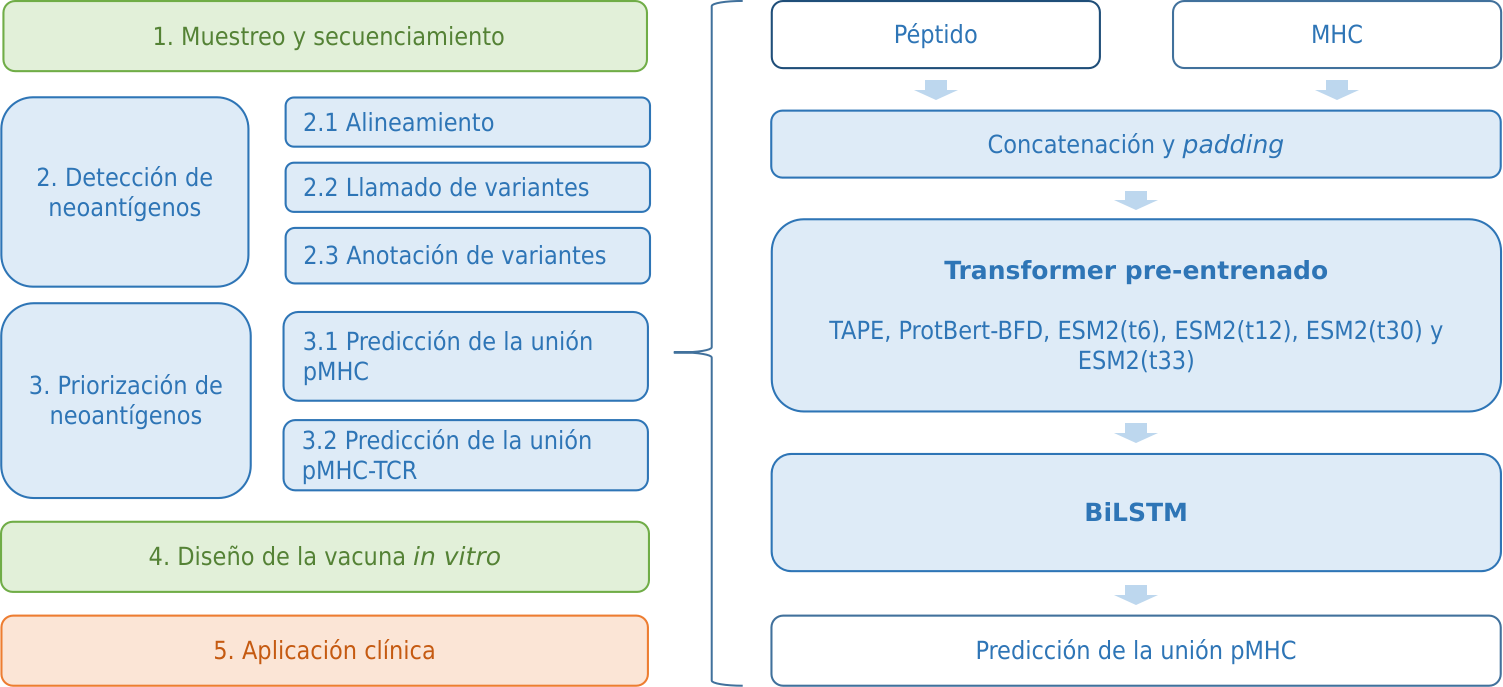
\includegraphics[width=\textwidth]{img/proposal/proposal}	
	\caption{Propuesta de \textit{transfer learning} de ESM-1b y una red neuronal paralela para la predicción de la afinidad entre un péptido y MHC (peptide MHC binding).}
	\label{fig:proposal}
\end{figure}


\section{Bases de datos}
Utilizamos secuencias de péptidos del conjunto de datos Anthem \citep{mei2021anthem}. Este conjunto de datos consta de 539,019 muestras para entrenamiento, 179,673 para validación y 172,580 para pruebas. Por ejemplo, en la Tabla \ref{tab:db_samples}, mostramos algunas muestras de esta base de datos. La columna MHC especifica el tipo de MHC o HLA, luego la columna pseudosecuencia, representa la secuencia de aminoácidos del MHC; esta pseudosecuencia fue obtenida de la base de datos de NetMHCpan4.1. Seguidamente, prosigue la secuencia de aminoácidos del péptido. Finalmente, la ultima columna es la clase o etiqueta, tendrá un valor de uno cuando existe una unión entre el pMHC y cero en caso contrario.


Adicionalmente, en la Figura \ref{fig:samples}, presentamos la distribución de las muestras por \textit{k-mers}. En Bioinformática, se hace referencia al termino \textit{k-mer} para representar secuencias biológicas de ADN, ARN o proteínas. Para el caso específico de proteínas, una secuencia de \textit{8-mer}, defina que la proteína en cuestión esta compuesta por 8 aminoácidos. Para la base de datos utilizada en esta investigación, los péptidos de \textit{9-mers} constituyen la mayoría de las muestras; miesntras que los péoptidos \textit{14-mer} son los mas escazos. Además, estos péptidos \textit{14-mer}, usualmente presentan comportamientos distintos. Esto ha ocasionado que los umbrales utilizados por los clasificadores varia dependiendo del \textit{k-mer} y por tipo de clasificador. 




\begin{table}[H]
	\caption[Ejemplo de algunas muestras de la base de datos]{Ejemplo de algunas muestras de la base de datos. Cada MHC es representado por una pseudosecuencia procesadas por NetMHCpan4.1. Luego los péptidos son cadenas de aminoácidos entreo 8 a 14 amino ácidos. La clase o etiqueta es un cero si existe una unión entre el péptido y el MHC o cero en caso contrario.}
	\label{tab:db_samples}
	\scriptsize
	\setlength{\tabcolsep}{0.5em} % for the horizontal padding
	{\renewcommand{\arraystretch}{1.5}% for the vertical padding
	\begin{tabular}{llll}
		\hline
		\textbf{MHC}         & \textbf{Pseudosecuencia del MHC}                & \textbf{Péptido}        & \textbf{Clase} \\ \hline
		HLA-A*01:01 & YFAMYQENMAHTDANTLYIIYRDYTWVARVYRGY & LFGRDLSY       & 1     \\
		HLA-A*01:01 & YFAMYQENMAHTDANTLYIIYRDYTWVARVYRGY & TDKKTHLY       & 1     \\
		HLA-A*01:01 & YFAMYQENMAHTDANTLYIIYRDYTWVARVYRGY & RSDTPLIY       & 1     \\
		HLA-A*01:01 & YFAMYQENMAHTDANTLYIIYRDYTWVARVYRGY & NSDLVQKY       & 1     \\
		HLA-A*01:01 & YFAMYQENMAHTDANTLYIIYRDYTWVARVYRGY & LSDLLDWK       & 1     \\
		HLA-A*01:01 & YFAMYQENMAHTDANTLYIIYRDYTWVARVYRGY & LLQNDGFF       & 1     \\
		HLA-A*01:01 & YFAMYQENMAHTDANTLYIIYRDYTWVARVYRGY & DSDMQTLV       & 1     \\
		HLA-A*01:01 & YFAMYQENMAHTDANTLYIIYRDYTWVARVYRGY & TDYHVRVY       & 1     \\
		HLA-A*01:01 & YFAMYQENMAHTDANTLYIIYRDYTWVARVYRGY & VLDSEGYL       & 1     \\
		HLA-A*01:01 & YFAMYQENMAHTDANTLYIIYRDYTWVARVYRGY & SDFHNNRY       & 1     \\
		HLA-C*06:02 & YDSGYREKYRQADVNKLYLWYDSYTWAEWAYTWY & FDGRVVTRSYLEKQ & 0     \\
		HLA-C*06:02 & YDSGYREKYRQADVNKLYLWYDSYTWAEWAYTWY & KPCCPDIDIFVDGK & 0     \\
		HLA-C*06:02 & YDSGYREKYRQADVNKLYLWYDSYTWAEWAYTWY & QDLKDFMRQAGEVT & 0     \\
		HLA-C*06:02 & YDSGYREKYRQADVNKLYLWYDSYTWAEWAYTWY & EGYPKSKKQFFEEV & 0     \\
		HLA-C*06:02 & YDSGYREKYRQADVNKLYLWYDSYTWAEWAYTWY & GNHISALKRRYTRR & 0     \\
		HLA-C*06:02 & YDSGYREKYRQADVNKLYLWYDSYTWAEWAYTWY & RHLRTHTGEKPYVC & 0     \\
		HLA-C*06:02 & YDSGYREKYRQADVNKLYLWYDSYTWAEWAYTWY & RGLNGGITPLNSIS & 0     \\
		HLA-C*06:02 & YDSGYREKYRQADVNKLYLWYDSYTWAEWAYTWY & SDFALKNPFYSLEM & 0     \\
		HLA-C*06:02 & YDSGYREKYRQADVNKLYLWYDSYTWAEWAYTWY & ALDSGDASPGTWSG & 0     \\
		HLA-C*06:02 & YDSGYREKYRQADVNKLYLWYDSYTWAEWAYTWY & QLVLYMKAAQLLAA & 0    \\ \hline
	\end{tabular}}
\end{table}


\begin{figure}[]
	\centering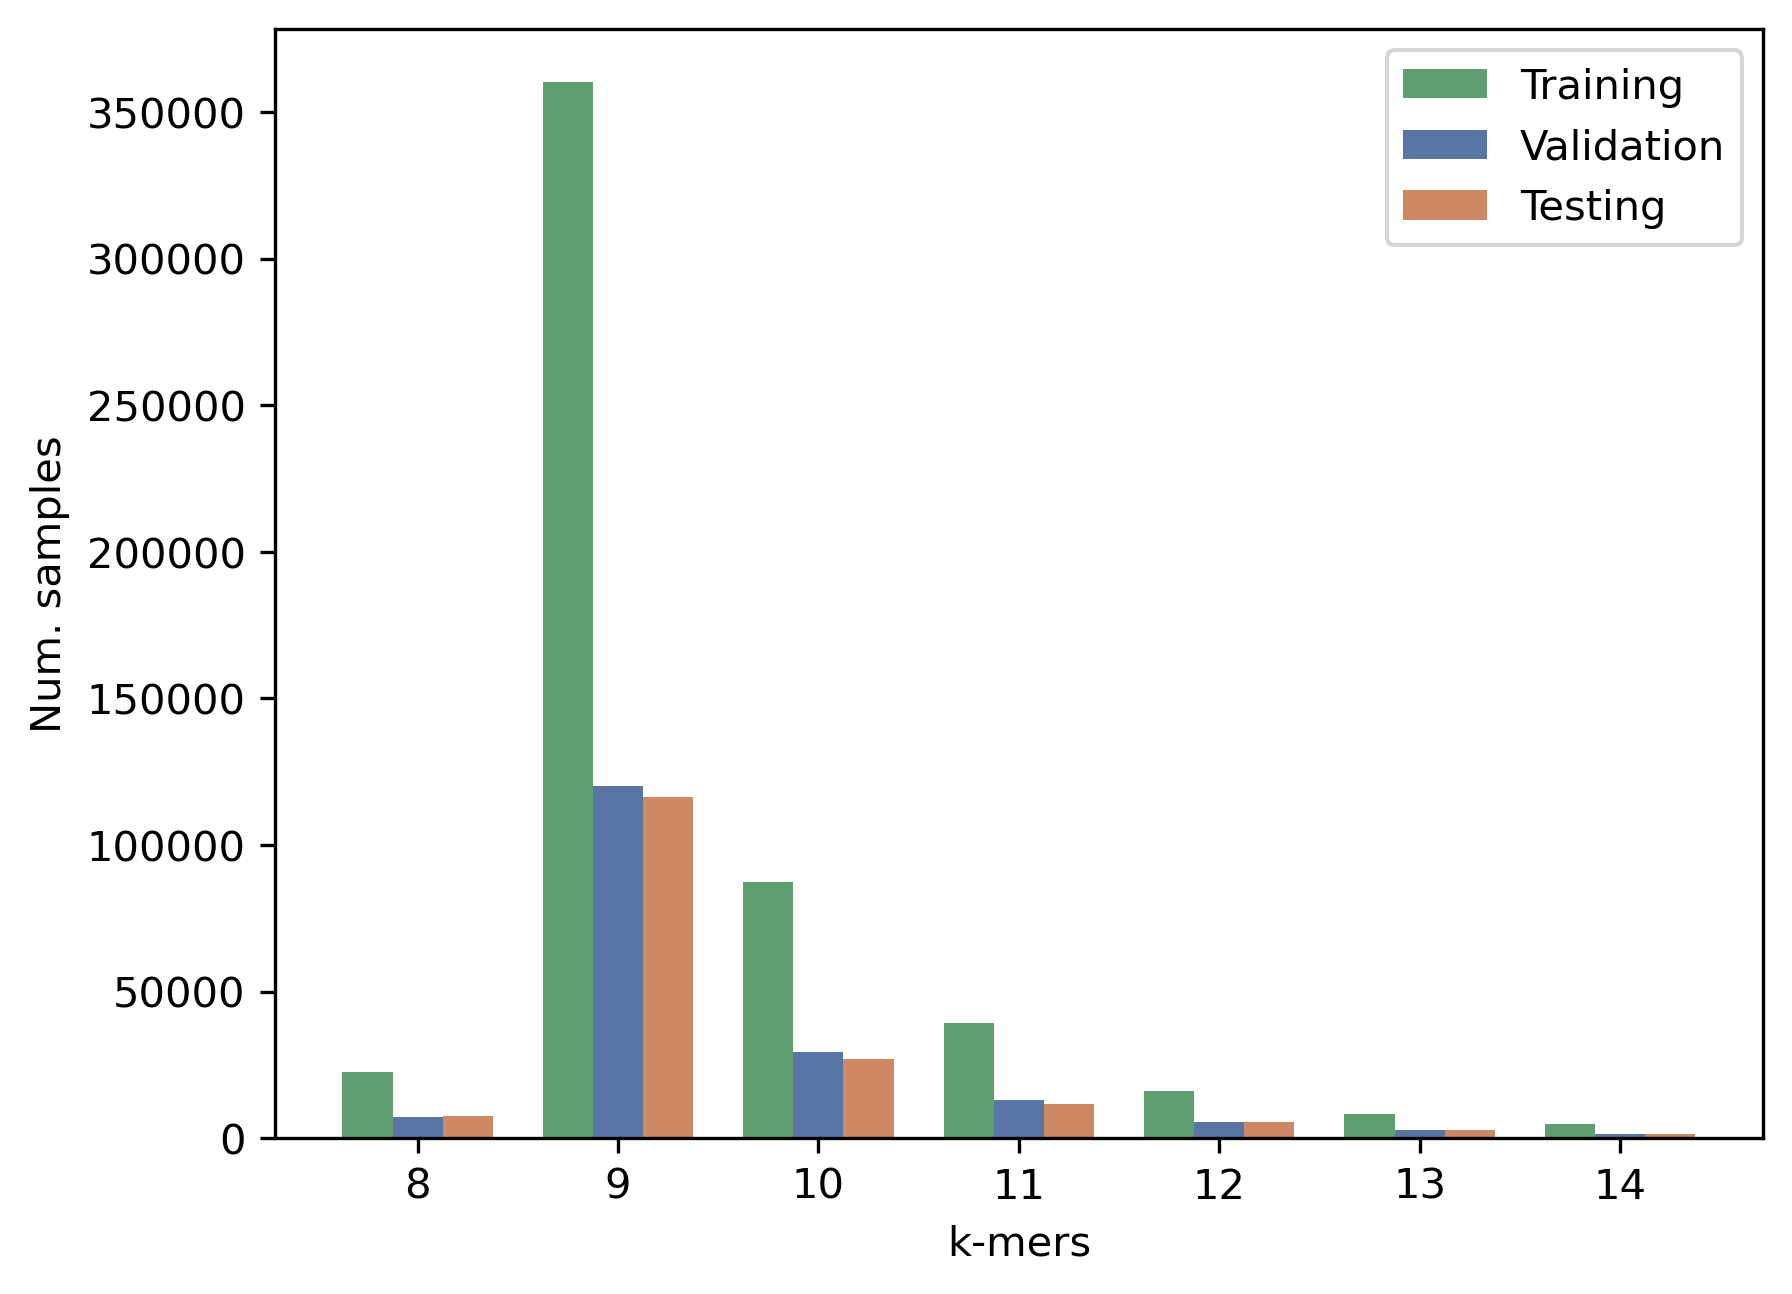
\includegraphics[width=0.8\textwidth]{img/proposal/dataset_samples}
	\caption{
		Cuantificación de las muestras por \textit{k-mers} dentro de los conjuntos de entrenamiento, validación y pruebas. El conjunto de datos se obtuvo de Anthem \cite{mei2021anthem}.}
	\label{fig:samples}
\end{figure}


\section{\textit{Transformer} pre-entrenados}

Evaluamos seis modelos de transformadores: TAPE \citep{rao2019evaluating}, ProtBert-BFD \citep{elnaggar2021prottrans} y ESM2 \citep{lin2023evolutionary} (ESM2(t6), ESM2(t12), ESM2(t30), ESM2(t33)). Estos modelos fueron entrenados con grandes conjuntos de datos de secuencias de proteínas como Pfam \citep{el2019pfam},  BFD y UniRef50 \citep{suzek2015uniref}. Además, se realizo \textit{fine-tuning } para la predicción de unión pMHC-I. En la Tabla \ref{tab:pretrained}, presentamos las características de cada modelo.

\begin{table}[t]%
	\centering
	\caption{Diferencias significativas entre los modelos TAPE, ProtBert-DFB y ESM2. HS: \textit{Hidden size}; AH: \textit{Attention heads}.}
	\label{tab:pretrained}%
	\setlength{\tabcolsep}{0.5em} % for the horizontal padding
	{\renewcommand{\arraystretch}{1.5}% for the vertical padding
	\begin{tabular}{llrrrrr}
		
		\textbf{Modelo}   & \textbf{BD} & \textbf{Muestras} & \textbf{Capas} & \textbf{HS} & \textbf{AH} & \textbf{Params.} \\
		\midrule
		TAPE             & Pfam             & 30M                   & 12              & 768                  & 12                       & 92M                 \\
		ProtBert-BFD     & BFD              & 2122M                 & 30              & 1024                 & 16                       & 420M                \\
		ESM2(t6)  & Uniref50         & 60M                   & 6               & 320                  & 20                       & 8M                  \\
		ESM2(t12)  & Uniref50         & 60M                   & 12              & 480                  & 20                       & 35M                 \\
		ESM2(t30) & Uniref50         & 60M                   & 30              & 640                  & 20                       & 150M                \\
		ESM2(t33)  & Uniref50         & 60M                   & 33              & 1280                 & 20                       & 650M               \\
		
	\end{tabular}}
	
\end{table}

\subsection{TAPE}


\textit{Tasks Assessing Protein Embeddings} (TAPE) \citep{rao2019evaluating} es el primer intento de evaluar el aprendizaje semi-supervisado en secuencias de proteínas. TAPE consta de doce capas de 512 unidades con ocho \textit{attention-heads}, lo que resulta en un total de 92 millones de parámetros. Los autores aplicaron entrenamiento semi-supervisado con la base de datos Pfam \citep{el2019pfam}, que contiene treinta millones de dominios de proteínas. Además, el conjunto de datos Pfam representa un subconjunto del \textit{Knowledge Base UniProt} (UniProtKB) \citep{uniprot2018uniprot}; en particular, Pfam utilizó secuencias de \textit{Reference Proteomes} \citep{finn2016pfam} en lugar de utilizar todo el conjunto de datos de UniProtKB. En consecuencia, Pfam tiene casi la mitad de las secuencias de proteínas que otras bases de datos extraídas de UniProtKB.

\subsection{ProtBert-BFD}

ProtBert-BFD es parte de una familia de modelos de ProtTrans \citep{elnaggar2021prottrans}. Los autores evaluaron varias arquitecturas de aprendizaje profundo con los conjuntos de datos BFD, UniRef50 y UniRef100, cada uno con 2122, 45 y 216 millones de secuencias. Añadido a esto, BFD se considera la colección más extensa de secuencias de proteínas; fusiona UniProt \citep{uniprot2019uniprot} y proteínas de múltiples proyectos de secuenciación de metagenómica. Mientras tanto, UniRef \citep{suzek2015uniref} proporciona un conjunto \textit{clusterized} de secuencias de proteínas de UniProtKB. Es importante destacar que el conjunto de datos más grande, BFD, las muestras tienen ruido y contiene errores en las secuencias \citep{elnaggar2021prottrans}.

Algunos de los modelos propuestos son ProtBert-BFD, ProtT5-XL y ProtT5-XXL, que tienen 420 millones, 3 mil millones y 11 mil millones de parámetros, respectivamente. ProtBert-BFD se entrenó con BFD; mientras tanto, los modelos ProtT5 se entrenaron inicialmente con BFD y luego con UniRef50, lo que mejoró el rendimiento en un 2.8\% y un 1.4\% para ProtT5-XL y ProtT5-XXL, respectivamente. Sin embargo, ProtT5-XL superó tanto a ProtBert-BFD como al modelo más grande, ProtT5-XXL. Los autores afirmaron que la cantidad de muestras mejoraba el rendimiento, pero no observaron una similitud consistente con el tamaño del modelo. Sugerían que modelos más grandes ven menos muestras con la misma potencia de cálculo, por lo que los modelos más grandes necesitan conjuntos de datos más grandes. Por esta razón, hemos optado por ProtBert, ya que es más pequeño que ProtT5-XL y creemos que se adapta mejor al tamaño del conjunto de datos actual para esta investigación.

\subsection{ESM2}


ESM-2 \citep{lin2023evolutionary} es una familia de modelos \textit{Transformer} que tienen  desde 8 millones hasta 15 billones de parámetros. El modelo se basa en BERT \citep{devlin2018bert} y supera a su versión anterior, ESM-1b \citep{rives2021biological}, al eliminar las capas de \textit{dropout} en las capas ocultas y de atención. Además, los autores sugirieron que los métodos de codificación de posición absoluta no se extrapolan bien; en consecuencia, utilizaron la \textit{Rotary Position Embedding} (RoPE). Significativamente, el uso de RoPE aumenta ligeramente el costo de entrenamiento; al mismo tiempo, mejora la calidad del modelo para modelos pequeños \citep{lin2023evolutionary}. Además, los autores utilizaron el conjunto de datos no redundante UniRef50 \citep{suzek2015uniref} de UniProt, que contiene 60 millones de secuencias de proteínas.


\section{\textit{Fine-tuning}}\label{sec:fine-tuned}

Una manera de realizar \textit{transfer learning} de modelos de \textit{deep learning} grandes, es realizando \textit{fine-tuning}. Está metodología, generalmente se aplica cuando tenemos un modelo entrenado con una base de datos muy grande, como por ejemplo una base de datos de texto de todas las páginas de internet. Luego, queremos adaptar dicho modelo para una tarea específica y en donde no contamos una base de datos muy grande, como por ejemplo un conjunto de muetras de análisis de sentimientos; entonces, podemos aplicar \textit{fine-tuning} al modelo entrenado con todo el texto de internet para una nueva tarea, entrenandolo de nuevo pero esta vez con el objetivo de predecir el sentimiento de un texto. En resumen está técnica consiste en modificar las ultimas capas del modelo pre-entrenado. La modificación puede ser eliminando las ultimas capas y agregando capas lineales, convoluciones, o recurrentes. Luego, se vuelve a entrenar el modelo una vez mas con el objetivo que el modelo se adapte al nuevo problema. En la Figura \ref{fig:fine-tuning}, mostramos un ejemplo de este procedimiento.

Luego, se sabe que al entrenar modelos de \textit{Transformers} grandes, las capas finales experimentan cambios más significativos, mientras que las capas iniciales, más cercanas a la entrada, sufren modificaciones relativamente menores. En otras palabras, las ultimas capas son mas específicas, mientras que las capas iniciales, representan caraterísticas generales del problema \citep{merchant2020happens,lee2019would,kovaleva2019revealing}. Debido a esto, es comun en los procesos de f\textit{ine-tuning}, eliminar las ultimas capas y agregar otras capas al final del modelo. En este trabajo,  apilamos en cascada un bloque BiLSTM al final del modelo pre-entrenado (ver Figura \ref{fig:fine-tuning_proposal}), luego se agrego una capa lineal con dos neuronas como salida para el problema de clasificación pMHC. Finalmente, este modelo se entreno con una base de datos de muestras de pMHC. Las características de los modelos BERT pre-entrenados se detallan en la Tabla \ref{tab:pretrained} mientras que las características del bloque LSTM utilizado en el proceso de \textit{fine-tuning} fueron inspirados por el trabajo de \cite{zhang2022hlab} y se detallan en la Tabla \ref{tab:biLSTM}.

 



\begin{figure}[H]
	\centering
	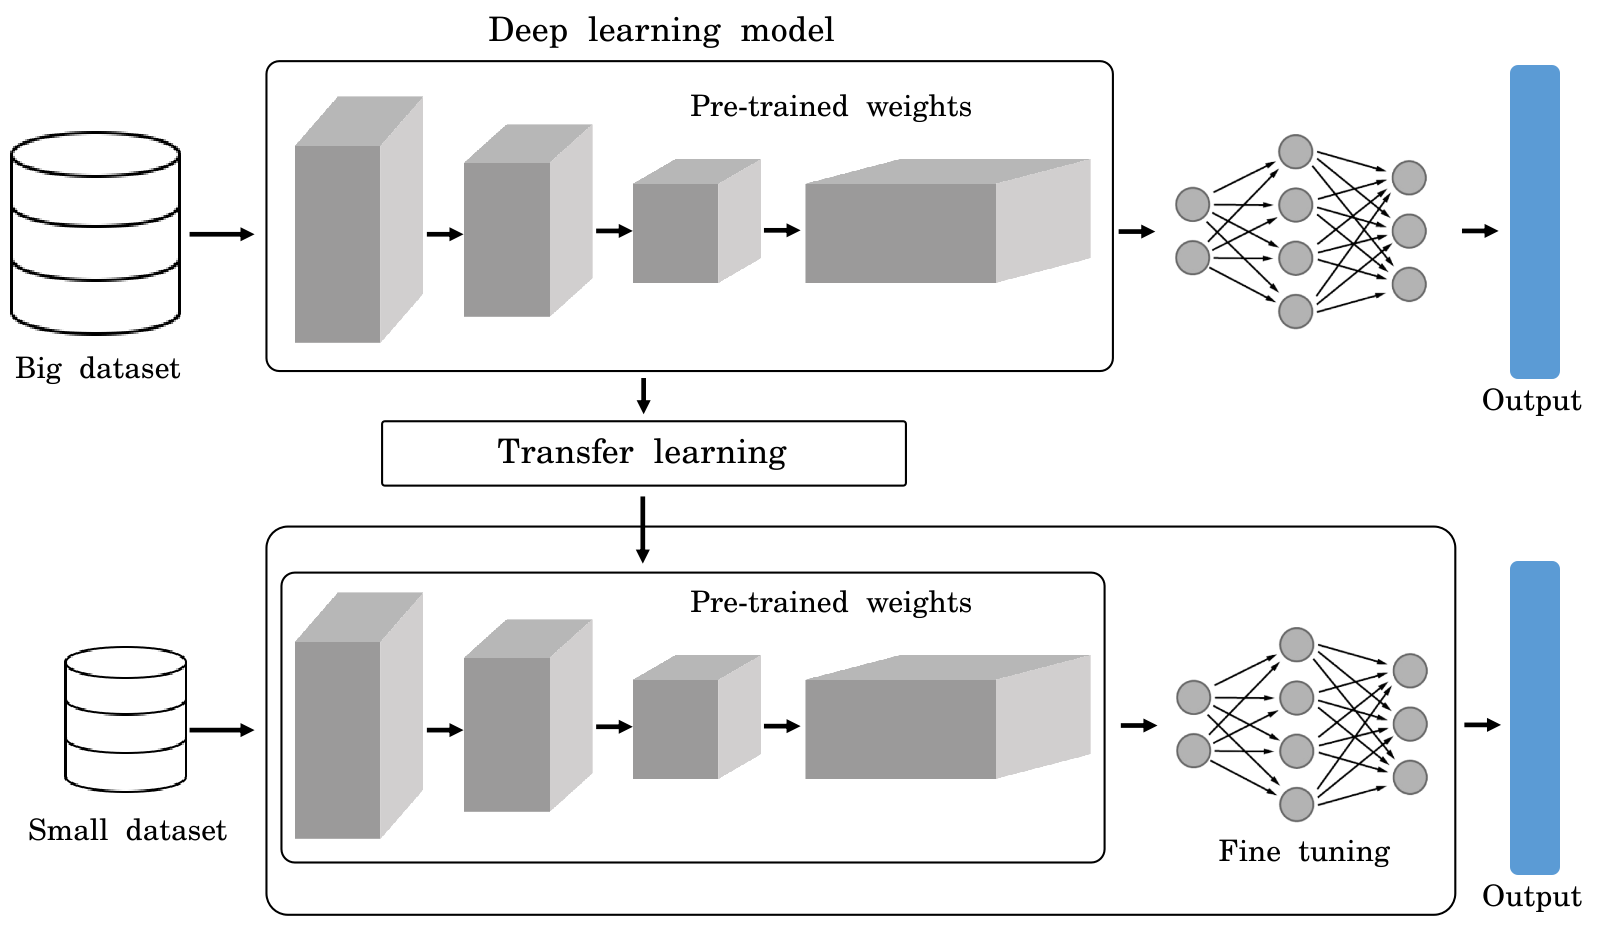
\includegraphics[width=\textwidth]{../img/proposal/fine_tuning}	
	\caption[Ejemplo de aplicación de \textit{Fine-tuning}]{Ejemplo de aplicación de \textit{Fine-tuning}. Primero, se entrena un modelo para una tarea $x$ con una gran base de datos, luego puede aprovecharse ese aprendizaje para otra tarea similar $y$ que no tenga una base de datos grande. Generalmente, en este proceso, se eliminan las ultimas capas y se agregan otras capas lineales, convoluciones o recurrentes. Fuente: Adaptado de  \cite{prince2023understanding}.}		
	\label{fig:fine-tuning}
\end{figure}


\begin{figure}[H]
	\centering
	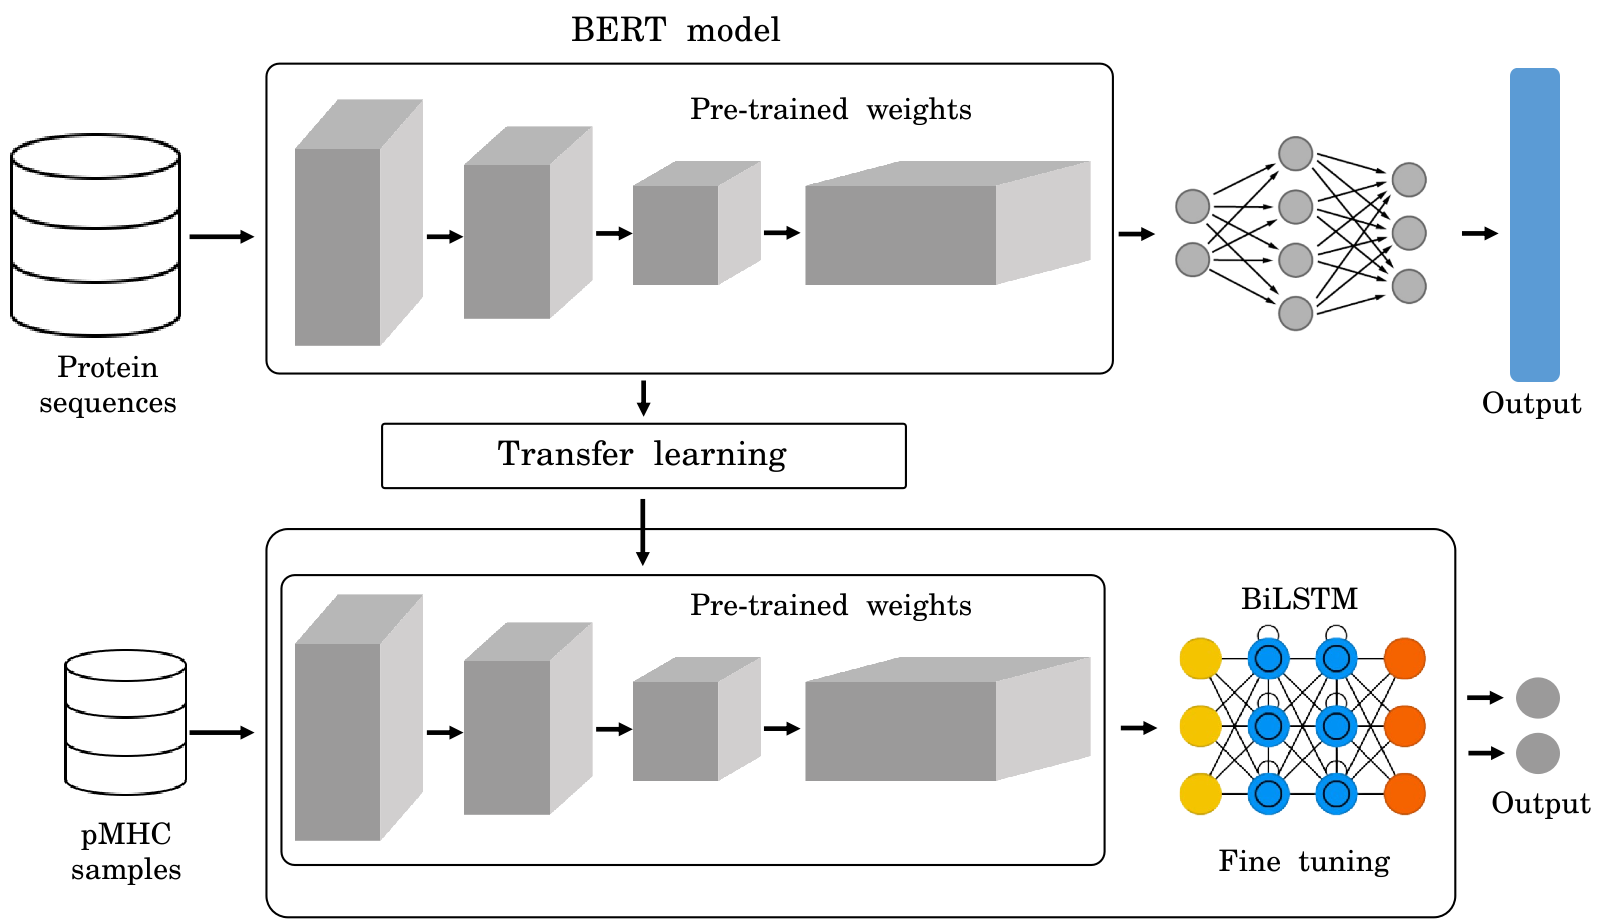
\includegraphics[width=\textwidth]{../img/proposal/fine_tuning_proposal}	
	\caption[Fine-tuning al modelo BERT]{\textit{Fine-tuning} propuesto. Se toma las primeras capas de un modelo BERT pre-entrenado con bases de datos de secuencias de proteínas. Luego, se agrega un bloque de capas BiLSTM al final y se entrena de nuevo con una base de datos pequeña de muestras pMHC. Fuente: Adaptado de  \cite{prince2023understanding}.}		
	\label{fig:fine-tuning_proposal}
\end{figure}
% agregar una figura especifica del finetuning




\begin{table}[t]%
	\centering
	\caption{Características del bloque BiLSTM utilizado en el \textit{fine-tuning}.}
	\label{tab:biLSTM}%
	\setlength{\tabcolsep}{0.5em} % for the horizontal padding
	{\renewcommand{\arraystretch}{1.5}% for the vertical padding
		\begin{tabular}{lp{9cm}p{1cm}p{1cm}}
			\hline
			\textbf{Tipo}   & \textbf{Entada} & \textbf{Salida}& \textbf{Capas} \\ \hline
			
			BiLSTM & Salida del modelo BERT (Tabla \ref{tab:pretrained}, columna HS) & 768 & 2 \\
			
			Dropout & 0.1\% & - & - \\
			Lineal & 1536 & 2 & 1 \\ \hline
	\end{tabular}}
	
\end{table}



\section{\textit{Gradient Accumulation Steps}}\label{sec:gas}

Adicionalmente, los modelos de \textit{Transformer} grandes utilizan bastante memoria de la GPU. Por lo tanto, inspirados en trabajos similares sobre entrenamiento de modelos grandes de \textit{Transformers} para problemas de NLP \citep{anil2021large,zhang2023adam,huang2023measuring}, evaluamos los resultados de aplicar \textit{Gradient Accumulation Steps} durante el entrenamiento. El proceso se explica en la Figura \ref{fig:gas_example}, por ejemplo en un entrenamiento normal durante el proceso de actualización de parámetros en el algoritmo de aprendizaje, se considera un solo \textit{mini-batch} para obtener las gradientes y luego actualiza los parametros; mientras que en el enfoque utilizando \textit{Gradient Accumulation Steps}, se consideran varios \textit{mini-batchs}, se suman sus gradientes y luego estas gradientes acumuladas son utilizadas para actualizar los parametros.



\begin{figure}[H]
	\centering
	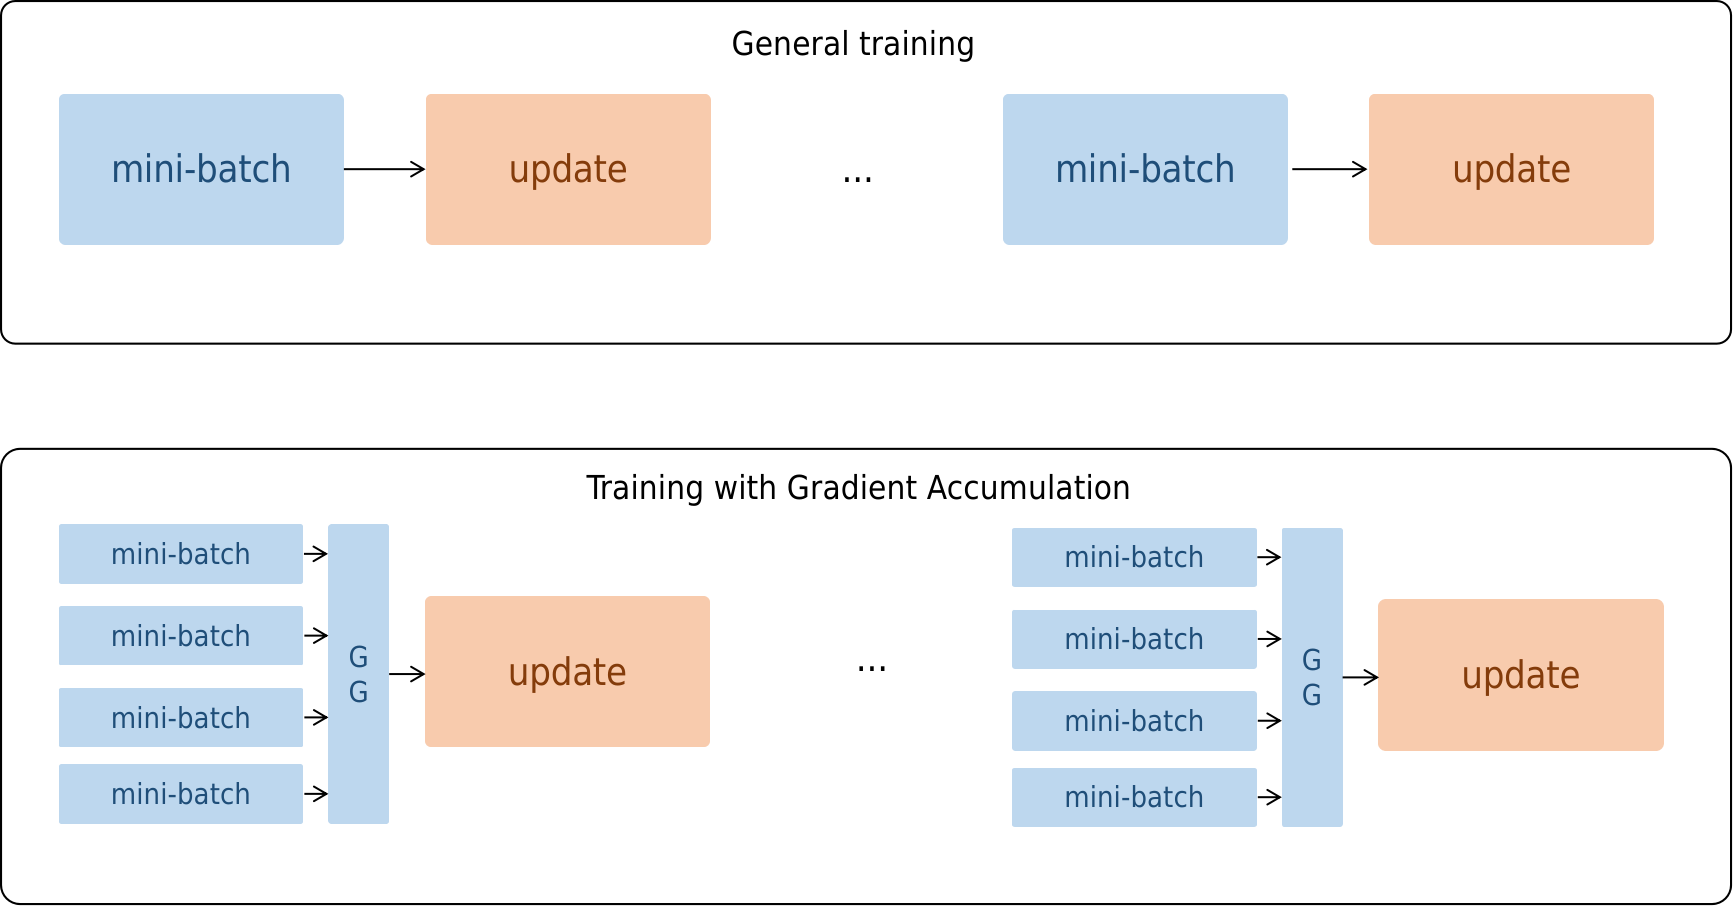
\includegraphics[width=\textwidth]{../img/proposal/gas_own}	
	\caption[Ejemplo de aplicación de \textit{Gradient Accumulation Steps}]{Ejemplo de aplicación de \textit{Gradient Accumulation Steps} durante el entranamiento de modelos de Deep Learning. En este caso, un entrenamiento general considera un solo \textit{mini-batch} para obtener las gradientes y luego actualiza los parámetros; mientras que en el enfoque utilizando \textit{Gradient Accumulation Steps}, se consideran varios \textit{mini-batchs}, se suman sus gradientes, luego estas gradientes acumuladas son utilizadas para actualizar los parámetros.  Fuente: Adaptado de  \cite{prince2023understanding}.}		
	\label{fig:gas_example}
\end{figure}



\section{Hiperparámetros}\label{sec:hyperparam}
Finalmente, utilizamos los siguientes hiperparámetros: tasa de aprendizaje de 5e-5, \textit{weight decay} de 0.0001, \textit{momentum} de 0.9, \textit{warn-up steps} de 1000 con \textit{linear decay}, optimizador ADAM ($\beta_1 = 0.9, \beta_2=0.999$) y \textit{early stopping}. Estos valores fueron utilizados por BERTMHC \citep{cheng2021bertmhc} después de buscar los mejores parámetros utilizando \textit{grid search}.

\section{Ambiente de trabajo}

\section{Clasificación binaria y Métricas}

El problema de predicción de unión pMHC es un problema de regresión. Sin embargo, basado en el conjunto de datos utilizado en este estudio, también podría abordarse como un problema de clasificación binaria al seleccionar un umbral apropiado. Las métricas de aprendizaje automático utilizadas en este trabajo son: \textit{accuracy, precision, recall, f-1 score, Area Under the Curve (AUC)}, y \textit{Matthews Correlation Coefficient} (MCC). Todas las métricas están descritas en las ecuaciones siguientes.

\begin{equation}\label{equa:acc}
	Accuracy = \frac{TP+TN}{TP+TN+FP+FN}
\end{equation}

\begin{equation}\label{equa:precision}
	Precision = \frac{TP}{TP+FP}
\end{equation}

\begin{equation}\label{equa:recall}
	Sensitivity = Recall = \frac{TP}{TP+FN}
\end{equation}

\begin{equation}\label{equa:f1}
	F1 = \frac{2*Precision*Recall}{Precision+Recall} = \frac{2 \times TP}{2*TP+FP+FN}
\end{equation}


\begin{equation}\label{equa:FPR}
	Specificity = \frac{TN}{FP+TN}
\end{equation}

\begin{equation}\label{equa:MCC}
	MCC = \frac{TP \times TN - FP \times FN}{ \sqrt{ (TP+FP)(TP  + FN)(TN+FP)(TN+FN)}  }
\end{equation}

donde \textit{TP}, hace referencia a la cantidad de muestras que eran verdaderas y han sido reconocidas como verdaderas; \textit{TN}, hace referencia a la cantidad de muestras que eran verdaderas y han sido reconocidas como falsas; \textit{FP}, son las muestras que eran falsas, pero fueron reconocidas como verdaderas; \textit{FN}, son las muestras que eran falsas y fueron reconocidas como falsas.
 % Introduction
%% ------------------------------------------------------------------- %%
%% ------------------------------------------------------------------- %%
%% ------------------------------------------------------------------- %%
%% ------------------------------------------------------------------- %%
\chapter{Resultaods}
\label{cap:resultados}


%% ------------------------------------------------------------------- %%
%% ------------------------------------------------------------------- %%
%% ------------------------------------------------------------------- %%
%% ------------------------------------------------------------------- %%
%% ------------------------------------------------------------------- %%
%% ------------------------------------------------------------------- %%

%% -------------------------------------------------------------------- %%
%% -------------------------------------------------------------------- %%



%EOF
 % Introduction
%% ------------------------------------------------------------------------- %%
\chapter{Conclusiones}
\label{cap:conclusiones}
\lhead{\emph{Introducción}}  



Primera: Se ha realizado una búsqueda sistemática de la literatura sobre los principales métodos basados en \textit{deep learning}, utilizados para la detección de neo antígenos. Estos métodos involucran las \textit{Shallow Neural Networks}, redes neuronales convolucionales, redes neuronales recurrentes y recientemente las redes \textit{Transformers} y BERT.


Segunda: Se ha presentado un nuevo método basado en redes neuronales BERT y con \textit{trasnfer lerning}, de los modelos pre entrenados TAPE y ESMb-1. El método propuesto ha sido evaluado con colección de varias muestras tomadas de bases de datos públicas y trabajos similares.



 % Introduction

%\input{Chapters/Chapter2} % Background Theory 

%\input{Chapters/Chapter3} % Experimental Setup

%\input{Chapters/Chapter4} % Experiment 1

%\input{Chapters/Chapter5} % Experiment 2

%\input{Chapters/Chapter6} % Results and Discussion

%\input{Chapters/Chapter7} % Conclusion



%% ---------------------------------------------------------------- APENDICES ----------------------------------------------------------
%% ----------------------------------------------------------------
% Now begin the Appendices, including them as separate files

%\addtocontents{toc}{\vspace{2em}} % Add a gap in the Contents, for aesthetics

%\appendix % Cue to tell LaTeX that the following 'chapters' are Appendices

%\chapter{An Appendix}

Lorem ipsum dolor sit amet, consectetur adipiscing elit. Vivamus at pulvinar nisi. Phasellus hendrerit, diam placerat interdum iaculis, mauris justo cursus risus, in viverra purus eros at ligula. Ut metus justo, consequat a tristique posuere, laoreet nec nibh. Etiam et scelerisque mauris. Phasellus vel massa magna. Ut non neque id tortor pharetra bibendum vitae sit amet nisi. Duis nec quam quam, sed euismod justo. Pellentesque eu tellus vitae ante tempus malesuada. Nunc accumsan, quam in congue consequat, lectus lectus dapibus erat, id aliquet urna neque at massa. Nulla facilisi. Morbi ullamcorper eleifend posuere. Donec libero leo, faucibus nec bibendum at, mattis et urna. Proin consectetur, nunc ut imperdiet lobortis, magna neque tincidunt lectus, id iaculis nisi justo id nibh. Pellentesque vel sem in erat vulputate faucibus molestie ut lorem.

Quisque tristique urna in lorem laoreet at laoreet quam congue. Donec dolor turpis, blandit non imperdiet aliquet, blandit et felis. In lorem nisi, pretium sit amet vestibulum sed, tempus et sem. Proin non ante turpis. Nulla imperdiet fringilla convallis. Vivamus vel bibendum nisl. Pellentesque justo lectus, molestie vel luctus sed, lobortis in libero. Nulla facilisi. Aliquam erat volutpat. Suspendisse vitae nunc nunc. Sed aliquet est suscipit sapien rhoncus non adipiscing nibh consequat. Aliquam metus urna, faucibus eu vulputate non, luctus eu justo.

Donec urna leo, vulputate vitae porta eu, vehicula blandit libero. Phasellus eget massa et leo condimentum mollis. Nullam molestie, justo at pellentesque vulputate, sapien velit ornare diam, nec gravida lacus augue non diam. Integer mattis lacus id libero ultrices sit amet mollis neque molestie. Integer ut leo eget mi volutpat congue. Vivamus sodales, turpis id venenatis placerat, tellus purus adipiscing magna, eu aliquam nibh dolor id nibh. Pellentesque habitant morbi tristique senectus et netus et malesuada fames ac turpis egestas. Sed cursus convallis quam nec vehicula. Sed vulputate neque eget odio fringilla ac sodales urna feugiat.

Phasellus nisi quam, volutpat non ullamcorper eget, congue fringilla leo. Cras et erat et nibh placerat commodo id ornare est. Nulla facilisi. Aenean pulvinar scelerisque eros eget interdum. Nunc pulvinar magna ut felis varius in hendrerit dolor accumsan. Nunc pellentesque magna quis magna bibendum non laoreet erat tincidunt. Nulla facilisi.

Duis eget massa sem, gravida interdum ipsum. Nulla nunc nisl, hendrerit sit amet commodo vel, varius id tellus. Lorem ipsum dolor sit amet, consectetur adipiscing elit. Nunc ac dolor est. Suspendisse ultrices tincidunt metus eget accumsan. Nullam facilisis, justo vitae convallis sollicitudin, eros augue malesuada metus, nec sagittis diam nibh ut sapien. Duis blandit lectus vitae lorem aliquam nec euismod nisi volutpat. Vestibulum ornare dictum tortor, at faucibus justo tempor non. Nulla facilisi. Cras non massa nunc, eget euismod purus. Nunc metus ipsum, euismod a consectetur vel, hendrerit nec nunc.	% Appendix Title

%\input{Appendices/AppendixB} % Appendix Title

%\input{Appendices/AppendixC} % Appendix Title

%\addtocontents{toc}{\vspace{2em}}  % Add a gap in the Contents, for aesthetics
%\backmatter

%% ----------------------------------------------------------------
%% ----------------------------------------------------------------
%% --------------------------------------------------------------------------------------------------------------------------


\label{Bibliography}
\lhead{\emph{Bibliografía}}  % Change the left side page header to "Bibliography"
%\bibliographystyle{unsrtnat}  % Use the "unsrtnat" BibTeX style for formatting the Bibliography
\bibliographystyle{apalike}  % Use the "unsrtnat" BibTeX style for formatting the Bibliography
%\bibliography{../Bibliography}  % The references (bibliography) information are stored in the file named "Bibliography.bib"
\bibliography{../bibliography_thesis}  % The references (bibliography) information are stored in the file named "Bibliography.bib"

\end{document}  % The End
%% ----------------------------------------------------------------